% Template for PLoS
% Version 3.4 January 2017
%
% % % % % % % % % % % % % % % % % % % % % %
%
%--IMPORTANT NOTE
%
% This template contains comments intended 
% to minimize problems and delays during our production 
% process. Please follow the template instructions
% whenever possible.
%
% % % % % % % % % % % % % % % % % % % % % % % 
% Once your paper is accepted for publication, 
% PLEASE REMOVE ALL TRACKED CHANGES in this file 
% and leave only the final text of your manuscript. 
% PLOS recommends the use of latexdiff to track changes during review, as this will help to maintain a clean tex file.
% Visit https://www.ctan.org/pkg/latexdiff?lang=en for info or contact us at latex@plos.org.
%
%
% There are no restrictions on package use within the LaTeX files except that 
% no packages listed in the template may be deleted.
%
% Please do not include colors or graphics in the text.
%
% The manuscript LaTeX source should be contained within a single file (do not use \input, \externaldocument, or similar commands).
%
% % % % % % % % % % % % % % % % % % % % % % %
%
%--FIGURES AND TABLES
%
% Please include tables/figure captions directly after the paragraph where they are first cited in the text.
%
% DO NOT INCLUDE GRAPHICS IN YOUR MANUSCRIPT
% - Figures should be uploaded separately from your manuscript file. 
% - Figures generated using LaTeX should be extracted and removed from the PDF before submission. 
% - Figures containing multiple panels/subfigures must be combined into one image file before submission.
% For figure citations, please use "Fig" instead of "Figure".
% See http://journals.plos.org/plosone/s/figures for PLOS figure guidelines.
%
% Tables should be cell-based and may not contain:
% - spacing/line breaks within cells to alter layout or alignment
% - do not nest tabular environments (no tabular environments within tabular environments)
% - no graphics or colored text (cell background color/shading OK)
% See http://journals.plos.org/plosone/s/tables for table guidelines.
%
% For tables that exceed the width of the text column, use the adjustwidth environment as illustrated in the example table in text below.
%
% % % % % % % % % % % % % % % % % % % % % % % %
%
%--EQUATIONS, MATH SYMBOLS, SUBSCRIPTS, AND SUPERSCRIPTS
%
% IMPORTANT
% Below are a few tips to help format your equations and other special characters according to our specifications. For more tips to help reduce the possibility of formatting errors during conversion, please see our LaTeX guidelines at http://journals.plos.org/plosone/s/latex
%
% For inline equations, please be sure to include all portions of an equation in the math environment.  For example, x$^2$ is incorrect; this should be formatted as $x^2$ (or $\mathrm{x}^2$ if the romanized font is desired).
%
% Do not include text that is not math in the math environment. For example, CO2 should be written as CO\textsubscript{2} instead of CO$_2$.
%
% Please add line breaks to long display equations when possible in order to fit size of the column. 
%
% For inline equations, please do not include punctuation (commas, etc) within the math environment unless this is part of the equation.
%
% When adding superscript or subscripts outside of brackets/braces, please group using {}.  For example, change "[U(D,E,\gamma)]^2" to "{[U(D,E,\gamma)]}^2". 
%
% Do not use \cal for caligraphic font.  Instead, use \mathcal{}
%
% % % % % % % % % % % % % % % % % % % % % % % % 
%
% Please contact latex@plos.org with any questions.
%
% % % % % % % % % % % % % % % % % % % % % % % %

\documentclass[10pt,letterpaper]{article}
\usepackage[top=0.85in,left=2.75in,footskip=0.75in]{geometry}

% amsmath and amssymb packages, useful for mathematical formulas and symbols
\usepackage{amsmath,amssymb}

% Use adjustwidth environment to exceed column width (see example table in text)
\usepackage{changepage}

% Use Unicode characters when possible
\usepackage[utf8x]{inputenc}

% textcomp package and marvosym package for additional characters
\usepackage{textcomp,marvosym}

% cite package, to clean up citations in the main text. Do not remove.
\usepackage{cite}

% Use nameref to cite supporting information files (see Supporting Information section for more info)
\usepackage[hidelinks]{hyperref}
\usepackage{nameref}

% line numbers
\usepackage[right]{lineno}

% ligatures disabled
\usepackage{microtype}
\DisableLigatures[f]{encoding = *, family = * }

% color can be used to apply background shading to table cells only
\usepackage[table]{xcolor}

%\usepackage{color}
%\usepackage{soul}

% array package and thick rules for tables
\usepackage{array}


% for glossaries
\usepackage[xindy]{glossaries}

% for comments
\usepackage{todonotes}

% packages for algorithms in the document
\usepackage{algorithm}
\usepackage{caption}
\usepackage{algorithmic}

% create "+" rule type for thick vertical lines
\newcolumntype{+}{!{\vrule width 2pt}}

% create \thickcline for thick horizontal lines of variable length
\newlength\savedwidth
\newcommand\thickcline[1]{%
  \noalign{\global\savedwidth\arrayrulewidth\global\arrayrulewidth 2pt}%
  \cline{#1}%
  \noalign{\vskip\arrayrulewidth}%
  \noalign{\global\arrayrulewidth\savedwidth}%
}

% \thickhline command for thick horizontal lines that span the table
\newcommand\thickhline{\noalign{\global\savedwidth\arrayrulewidth\global\arrayrulewidth 2pt}%
\hline
\noalign{\global\arrayrulewidth\savedwidth}}


% Remove comment for double spacing
%\usepackage{setspace} 
%\doublespacing

% Text layout
\raggedright
\setlength{\parindent}{0.5cm}
\textwidth 5.25in 
\textheight 8.75in

% Bold the 'Figure #' in the caption and separate it from the title/caption with a period
% Captions will be left justified
\usepackage[aboveskip=1pt,labelfont=bf,labelsep=period,justification=raggedright,singlelinecheck=off]{caption}
\renewcommand{\figurename}{Fig}

\usepackage{mathtools}
\DeclarePairedDelimiter\abs{\lvert}{\rvert}%

% Improved C++ logo
\newcommand{\CC}{C\nolinebreak\hspace{-.05em}\raisebox{.4ex}{\tiny\bf +}\nolinebreak\hspace{-.10em}\raisebox{.4ex}{\tiny\bf +}}


% Use the PLoS provided BiBTeX style
\bibliographystyle{plos2015}

% Remove brackets from numbering in List of References
\makeatletter
\renewcommand{\@biblabel}[1]{\quad#1.}
\makeatother

% Leave date blank
\date{}

% Header and Footer with logo
\usepackage{lastpage,fancyhdr,graphicx}
\usepackage{epstopdf}
\pagestyle{myheadings}
\pagestyle{fancy}
\fancyhf{}
\setlength{\headheight}{27.023pt}
\lhead{
\includegraphics[width=2.0in]{PLOS-submission.eps}}
\rfoot{\thepage/\pageref{LastPage}}
\renewcommand{\footrule}{\hrule height 2pt \vspace{2mm}}
\fancyheadoffset[L]{2.25in}
\fancyfootoffset[L]{2.25in}
\lfoot{\sf PLOS}

%% Include all macros below

\newcommand{\lorem}{{\bf LOREM}}
\newcommand{\ipsum}{{\bf IPSUM}}

%\newcommand{\reviewertwo}[1]{\textcolor{red}{#1}}
%\newcommand{\reviewerfour}[1]{\textcolor{blue}{#1}}
%\newcommand{\reviewerfive}[1]{\textcolor{green}{#1}}

\definecolor{airforceblue}{rgb}{0.36, 0.54, 0.66}
\newcommand{\reviewertwo}[1]{\textcolor{airforceblue}{#1}}
\newcommand{\reviewerfour}[1]{\textcolor{airforceblue}{#1}}
\newcommand{\reviewerfive}[1]{\textcolor{airforceblue}{#1}}

%\newcommand{\reviewertwo}[1]{\textcolor{black}{#1}}
%\newcommand{\reviewerfour}[1]{\textcolor{black}{#1}}
%\newcommand{\reviewerfive}[1]{\textcolor{black}{#1}}

%\newcommand{\reviewertwo}[1]{\hl{#1}}
%\newcommand{\reviewerfour}[1]{\hl{#1}}
%\newcommand{\reviewerfive}[1]{\hl{#1}}

%% END MACROS SECTION





% this command generates the glossary:
\makeglossaries

\loadglsentries{acronyms.tex}





\begin{document}
\vspace*{0.2in}

% Title must be 250 characters or less.
\begin{flushleft}
{\Large
\textbf\newline{Phonetic Acquisition in Cortical Dynamics, a Computational Approach} % Please use "sentence case" for title and headings (capitalize only the first word in a title (or heading), the first word in a subtitle (or subheading), and any proper nouns).
}
\newline
% Insert author names, affiliations and corresponding author email (do not include titles, positions, or degrees).
\\
Dario Dematties\textsuperscript{1*},
Silvio Rizzi\textsuperscript{2},
George K. Thiruvathukal\textsuperscript{2,3},
Alejandro Wainselboim\textsuperscript{5},
B. Silvano Zanutto\textsuperscript{1,4} %,
%Name6 Surname\textsuperscript{2\ddag},
%Name7 Surname\textsuperscript{1,2,3*},
%with the Lorem Ipsum Consortium\textsuperscript{\textpilcrow}
\\
\bigskip
\textbf{1} Universidad de Buenos Aires, Facultad de Ingenier\'ia, Instituto de Ingenier\'ia Biom\'edica, Ciudad Aut\'onoma de Buenos Aires, Argentina
\\
\textbf{2} Argonne National Laboratory, Lemont, Illinois, United States
\\
\textbf{3} Computer Science Department, Loyola University Chicago, Chicago, Illinois, United States
\\
\textbf{4} Instituto de Biolog\'ia y Medicina Experimental-CONICET, Ciudad Aut\'onoma de Buenos Aires, Argentina
\\
\textbf{5} Instituto de Ciencias Humanas, Sociales y Ambientales, Centro Cient\'ifico Tecnol\'ogico-CONICET, Ciudad de Mendoza, Mendoza, Argentina
\\
\bigskip

% Insert additional author notes using the symbols described below. Insert symbol callouts after author names as necessary.
% 
% Remove or comment out the author notes below if they aren't used.
%
% Primary Equal Contribution Note
%\Yinyang These authors contributed equally to this work.

% Additional Equal Contribution Note
% Also use this double-dagger symbol for special authorship notes, such as senior authorship.
%\ddag These authors also contributed equally to this work.

% Current address notes
%\textcurrency Current Address: Dept/Program/Center, Institution Name, City, State, Country % change symbol to "\textcurrency a" if more than one current address note
% \textcurrency b Insert second current address 
% \textcurrency c Insert third current address

% Deceased author note
%\dag Deceased

% Group/Consortium Author Note
%\textpilcrow Membership list can be found in the Acknowledgments section.

% Use the asterisk to denote corresponding authorship and provide email address in note below.
* ddematties@fi.uba.ar
 

\end{flushleft}
% Please keep the abstract below 300 words
\section*{Abstract}

%I kept this copy of the old abstract just in case we need it again
%There are many computational theories that have been developed in order to improve artificial phonetic classification performance from linguistic auditory streams. However, less attention has been given to neurophysiological features recently found in cortical tissue. We focus on a context in which basic linguistic units--such as phonemes--are extracted and robustly classified by humans and other animals from complex acoustic streams in speech data. We introduce a biologically inspired and fully unsupervised neurocomputational approach that incorporates key neurophysiological and anatomical cortical properties. Its feature abstraction capabilities show promising phonetic invariance and generalization attributes. The model leverages the phonetic classification performance of the supervised \gls{svm} for monosyllabic, disyllabic and trisyllabic word classification tasks in the presence of environmental disturbances such as white noise, reverberation, and pitch variations. Thus, our computational model outperforms sophisticated multiresolution spectro-temporal auditory feature representations of phonetic linguistic streams of data.

\reviewertwo{Many computational theories have been developed to} improve artificial phonetic classification performance from linguistic auditory streams. However, less attention has been given to \reviewerfour{psycholinguistic data} and neurophysiological features recently found in cortical tissue. We focus on a context in which basic linguistic units–such as phonemes–are extracted and robustly classified by humans and other animals from complex acoustic streams in speech data. \reviewerfour{We are specially motivated by the fact that 8-month-old human infants can accomplish segmentation of words from fluent audio streams based exclusively on the statistical relationships between neighboring speech sounds without any kind of supervision}. In this paper, we introduce a biologically inspired and fully unsupervised neurocomputational approach that incorporates key neurophysiological and anatomical cortical properties, \reviewertwo{including columnar organization, spontaneous micro-columnar formation, adaptation to contextual activations and {\glspl{sdr}} produced by means of partial \gls{nmda} depolarization}. Its feature abstraction capabilities show promising phonetic invariance and generalization attributes. \reviewertwo{Our model improves the performance of a \gls{svm} classifier for} monosyllabic, disyllabic and trisyllabic word classification tasks in the presence of environmental disturbances such as white noise, reverberation, and pitch \reviewerfour{and voice} variations. \reviewerfour{Furthermore, our approach emphasizes potential self-organizing cortical principles achieving an improvement without any kind of optimization guidance which could minimize hypothetical loss functions by means of--for example--backpropagation}. Thus, our computational model outperforms multiresolution spectro-temporal auditory feature representations \reviewerfour{using only the statistical sequential structure immerse in the phonotactic rules of the input stream}.

% * <awainselboim@gmail.com> 2018-05-15T14:16:16.696Z:
%
% ^.

% This seems like a nice sentence for the author summary.
%This research has significant potential to open up new--and more biologically accurate--alternatives to overcome limitations in current deep feature extraction methods.

% Please keep the Author Summary between 150 and 200 words
% Use first person. PLOS ONE authors please skip this step. 
% Author Summary not valid for PLOS ONE submissions.   

\section*{Author summary}

%I kept this copy of the old author summary just in case we need it again
%Striking computational properties emerge from certain features of the mammalian cortex in general. Understanding how phonetic invariance and generalization can arise from such features is an outstanding challenge in neuroscience. Furthermore, overcoming this challenge could shed light on the mechanisms governing other modalities, given the anatomical and physiological uniformity found in cortical tissue. We base our work on a set of cortical features in the mammalian cortex which we believe could be relevant for invariance and generalization in phonetic perception. We incorporate such features in a computational model that shows to explain invariance and generalization in the classification of words with different number of syllables. The outcome is a computational model, inspired by the biology of cortical tissue, which can learn and robustly recognize the phonetic structure of words in the presence of different disturbances--not present during training--affecting the auditory stimulus. This research has significant potential to open up new--and more biologically accurate--alternatives to overcome limitations in current deep feature extraction methods.

Striking computational properties emerge from certain features of the mammalian cortex in general. Understanding how phonetic invariance and generalization can arise from such features is an outstanding challenge in neuroscience. Furthermore, overcoming this challenge could shed light on the mechanisms governing other modalities, given the anatomical and physiological uniformity found in cortical tissue. We base our work on a set of features in the mammalian cortex which we believe could be relevant for phonetic perception invariance and generalization \reviewerfour{in the absence of any clue beyond the statistical regularity present in the input stream}. We incorporate such features \reviewertwo{in a computational model which we show improves invariance and generalization} in the classification of words with different number of syllables. The outcome is a computational model, inspired by the biology of cortical tissue, which can learn and robustly recognize the phonetic structure of words in the presence of different disturbances--not present during training--affecting the auditory stimulus. This research has significant potential to open up new--and more biologically accurate--alternatives to overcome limitations in current deep feature extraction methods.



\linenumbers

% Use "Eq" instead of "Equation" for equation citations.
\section*{Introduction}

% NOTE from GKT: I have removed the headings for each paragraph. It doesn't really help with the reading. Instead we
% now have key phrases with emphasis (emph).

% Also a bit of a word about LaTeX, I have found many paragraphs are not formatted nicely to take advantage of the editor
% wrapping. This makes it very hard to change the text. You will notice through all sections that I have edited thus far
% that each paragraph is now on a soft-wrapped line. There is no newline until the end of the paragraph. I will only use
% hard newlines on comments such as this.



It is well known that human beings can reliably discriminate phonemes as well as other linguistic units by categorizing them, despite considerable variability across different speakers with different pitches and prosody. Furthermore, this ability extends to noisy and reverberant environments.

\reviewerfive{Although such proficiency could in part be attributed to top-down information \cite{PMID:17451657} originated in the grammatical and semantic \cite{OBLESER2011713,10.1093/cercor/bhp128} dimensions present in human language--beyond the phonetic features in the speech signal}--trained animals are also able to discriminate phoneme pairs categorically and to generalize in novel situations~\cite{kuhl_1975, kuhl_1983, kluender_1998, pons_2006, hienz_1996, dent_1997, lotto_1997}. For instance, \reviewertwo{cortical activations in naive ferrets revealed the existence} of spectro-temporal tuning in \gls{a1} with the capacity of supporting discrimination of many American English phonemes \cite{mesgarani_2008}, even when stimuli were distorted by additive noise and reverberation \cite{mesgarani_2014A}.

%I added this paragraph to the intro
\reviewerfour{It is even more remarkable that an extremely complex task of early language acquisition as is the segmentation of words from fluent speech, is fulfilled by 8-month-old infants based simply on the statistical relationships between neighboring speech sounds \cite{Saffran1996StatisticalLB}. With only 2 minutes of exposure to a continuous speech stream generated by a speech synthesizer, infants showed succesful phonetic acquisition and discrimination. Furthermore, in the training phase there was no acoustic information about word boundaries beyond the statistical structure in the phonotactic rules immerse in the stimuli, and the subjects received no external associative supervision or reinforcement which could have guided or boosted the phonetic acquisition task, which was entirely incidental}.

% I hold this paragraph just in case we need it
%How can cortical tissue show such physiological properties in response to complex auditory streams? This \reviewerfour{incidentally acquired} invariance in phonetic perception found in mammals must be grounded necessarily in anatomical and neurophysiological characterisitcs of the mammalian cortex. The features we foresee as potentially relevant will be described in the following section.

\reviewerfour{This incidentally acquired invariance in phonetic perception found in mammals must be grounded necessarily in anatomical and neurophysiological characterisitcs of the mammalian cortex. The features we foresee as potentially relevant are brought together in order to pose our computational hypotheses}.






\subsection*{Anatomical and neurophysiological characteristics of mammalian cortex}

\reviewerfive{Linden and Schreiner \cite{linden_2003}
highlighted that although auditory cortical circuits have some unique characteristics which require special attention,
their similarities with other sensory regions--such as visual or somatosensory cortex--turn out to be categorical.
First, at the sensory level, the cochlear one-dimensional frequency map could be analogous to the two-dimensional spatial maps which are found
in the retina or body surface.
Second, the tonotopic maps found in the auditory system could be analogous to the retinotopic and somatotopic organization found in visual and somatosensory cortices,
respectively.
Frequency tuning curves in the auditory system could correspond to inhibition of spatial surrounding boundaries in visual and somatosensory receptive fields.
A correspondence could be drawn between amplitude modulation rate in the auditory system and flicker sensitivity in the visual system, or
whisker vibration sensitivity in the somatosensory system.
Finally, auditory receptive fields tuned for frequency-sweep, could be analogous to visual and somatosensory motion sensitivity}.

\reviewerfive{Compelling physiological studies have shown that \glsfirst{a1} shares common structural
characteristics with other sensory cortices.
Furthermore,  when retinal inputs are routed into the auditory thalamus, auditory cortical cells develop visual response properties such as direction selectivity, orientation preference and complex and simple receptive fields
\cite{Sur1437, doi:10.1002/(SICI)1096-9861(19981026)400:3<417::AID-CNE10>3.0.CO;2-O, Roe1992VisualPR}.
Retinotopic maps, in terms of orientation tuning with lateral connectivity between orientation domains, emerge in superficial layers of the rewired
auditory cortex \cite{Roe818, Sharma2000InductionOV}}.

\reviewerfive{The above data suggest the existence of neuronal circuitry with similar processing capabilities for different modalities. Consequently, we gather physiological and anatomical characteristics found in cortical tissue in general which we foresee as relevant for phonetic perception invariance and generalization}.

One of the main neuroanatomical features of brain cortex in mammals is that \reviewertwo{cortical cells are spacially arranged into domains defined by common receptive field locations}. These alignments are called \glspl{cc}~\cite{mountcastle_1955, mountcastle_1957, hubel_1962, hubel_1968}. Within \glspl{cc}, cortical mini-columns are clusters of cells which respond to stimuli with similar characteristics (Fig. \ref{fig:Biological}). In addition, cortical columns are connected within and between different regions in cortical tissue forming a complex and yet organized connectivity network~\cite{mountcastle_1997}. 

\begin{figure}[h!]
    \centering
    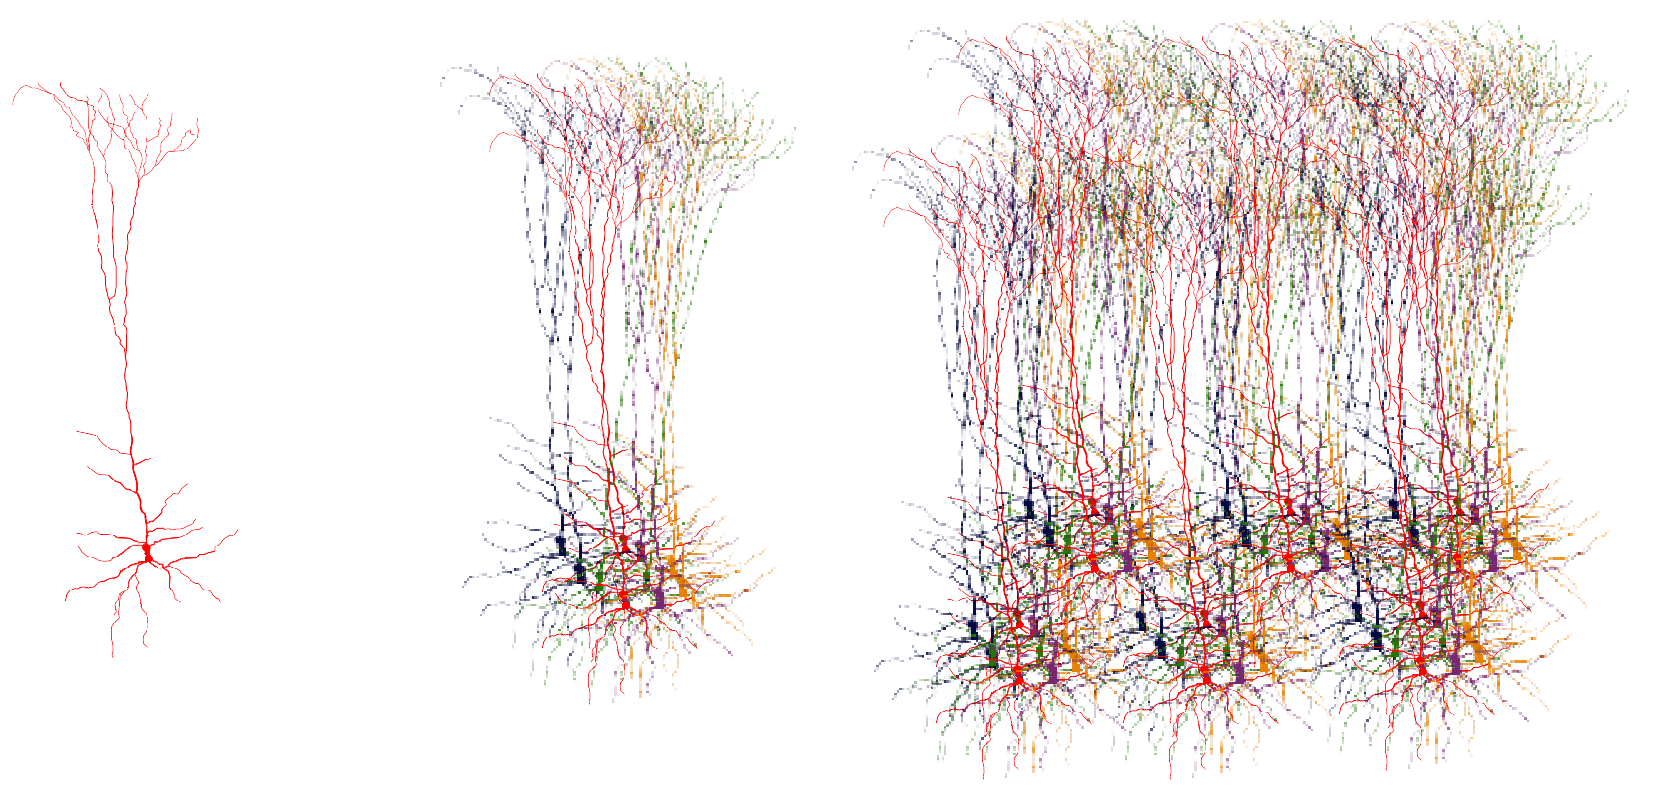
\includegraphics[width=1.0\textwidth]{Biological.png}
    \caption{Cortical tissue organization. Left: Pyramidal cell. The most common excitatory neuron in cortical tissue.
    Center: Cortical mini-column. A cluster on neural cells which responds to stimuli of similar characteristics.
    Right: Cortical Column. A group of mini-columns with a common receptive field location.
    Adapted from (Fabuio, Own work, CC BY 4.0, \url{https://commons.wikimedia.org/w/index.php?curid=60707501)}}
    \label{fig:Biological}
\end{figure}

One of the functional properties found in many of these networks is adaptation to contextual stimuli \cite{KRAUSE201436,doi:10.1167/16.13.1}. This mechanism is thought to enhance efficiency in the codification of sensory information. For instance, a reduction in the responses to frequent sounds by means of inhibitory networks, may enhance cortical sensitivity to rare sounds that may represent unexpected events~\cite{Natan2015ComplementaryCO,nachum_2003,Javitt11962}.

Finally, recent findings in neuroscience show that mammalian cortex processes information by means of \glspl{sdr}~\cite{barth_2012}. This mechanism allows robust and low-error-rate discrimination of stimuli representations minimizing the neuronal activation during the task in relation to the neural resources available for the representation~\cite{ahmad_2016}. Hawkins et al. \cite{hawkins_2016} hypothetize that one of the mechanisms that might be involved in cortical networks in order to achieve \glspl{sdr} implies the extended depolarization of the soma as the result of independent dendritic \gls{nmda} branch activations produced by the excitation of certain number of distal synapses~\cite{antic_2010, major_2013}.

\reviewerfive{In the present work the above mentioned anatomical and neurophysiological features of the mammalian cortex are gathered as potentially relevant in order to attain phonetic invariance in the mammalian auditory cortex. Our pyramidal neuron model dissociates proximal from distal dendritic branches (Fig.~\ref{fig:PyramidalCell}). Proximal dendrites act as a homogeneous set receiving only afferent information. Information in proximal dendrites determines a bunch of neural units in a \gls{cc} which could be activated depending on the previous activations in the same as well as in neighboring \glspl{cc}}.

\begin{figure}[h!]
    \centering
    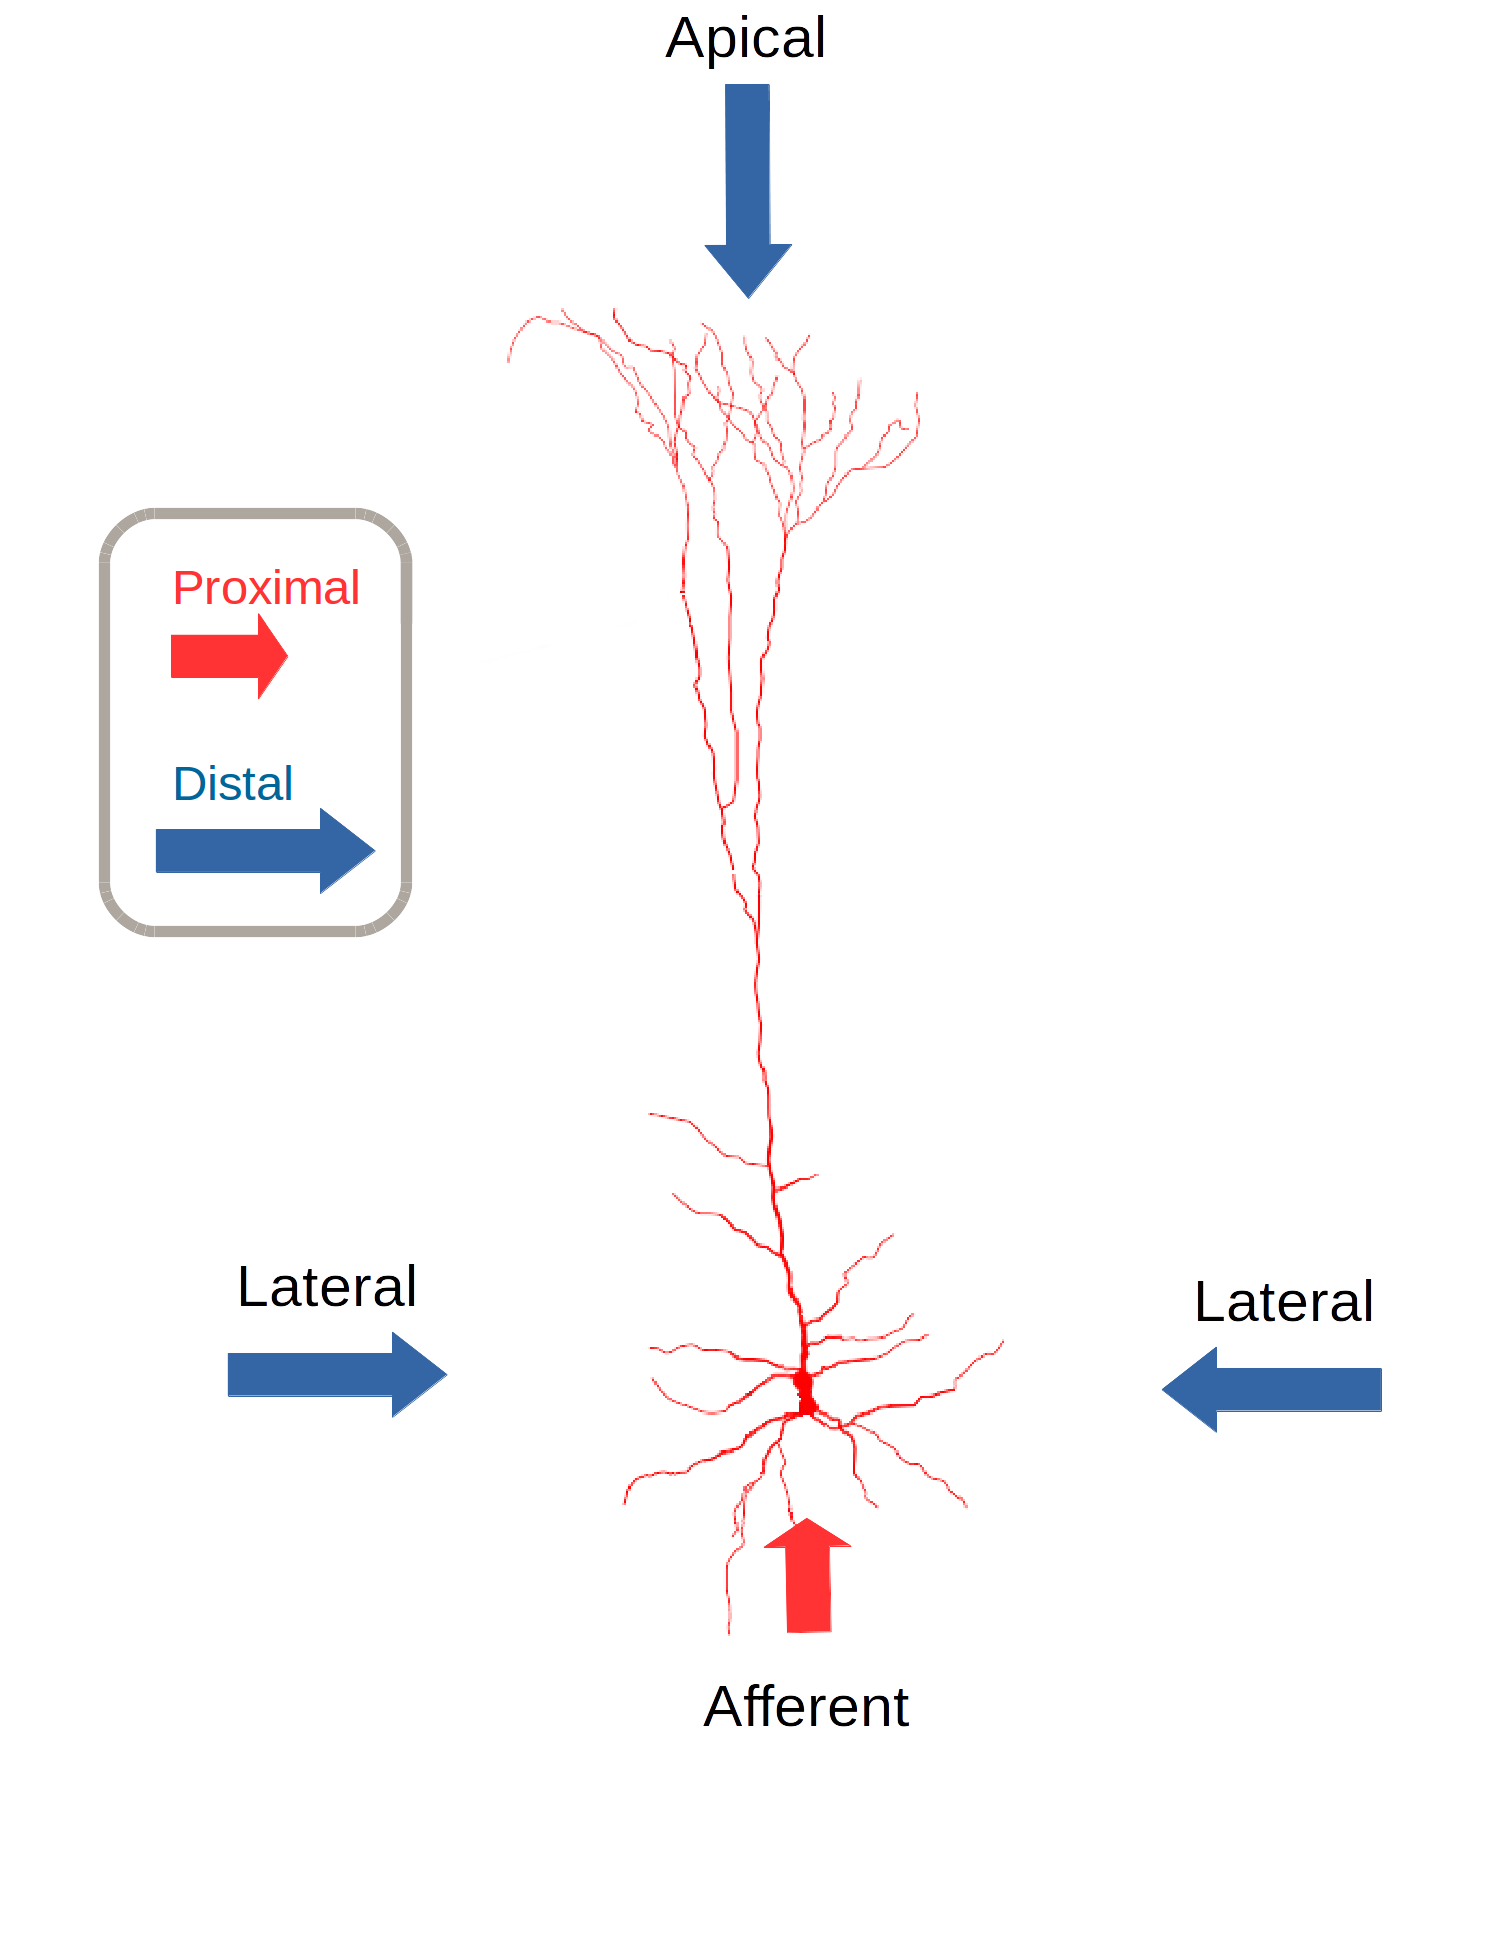
\includegraphics[width=0.5\textwidth]{PyramidalCell.png}
    \caption{Connectivity profile of a pyramidal neural unit in the \gls{el}.
    Proximal connections are formed only by afferent connections from the \gls{mrstsa}
    while distal connections are formed by lateral and apical connections from neighboring columns and
    from columns in another cortical layer above respectively.
    The \gls{el} is the most important stage in our computational approach while the \gls{mrstsa} pre-processes the audio corpora in order to feed the \gls{el}.
    Adapted from 
    (Fabuio - Own work, CC BY 4.0, \url{https://commons.wikimedia.org/w/index.php?curid=60707501)}}
    \label{fig:PyramidalCell}
\end{figure}

\reviewerfive{Distal dendrites receive only lateral and apical information acting as independent detectors. Distal dendritic information pre-activates neural units putting them in a predictive state in order to receive future afferent information}.

\reviewerfive{We test those principles paying special attention to temporal dynamics of speech, which play the most important role in linguistic contrasts~\cite{doi:10.1098/rstb.1992.0070}}. We use a completely unsupervised and \reviewertwo{biologically-inspired computational model,} \reviewerfour{since we aim to mimic infant incidental phonetic acquisition in whose circumstances no supervision could be justified}. \reviewertwo{Our model produces levels of phonetic classification accuracy} similar to those of state-of-the-art deep pattern classification approaches. We therefore propose an alternative path towards addressing phonetic discrimination based on observing structural and functional properties present in the mammalian cortex.


















\section*{Materials and methods}


\subsection*{Corpora generation}
\label{CorpGen}

We generate corpora of 500 words with mono, di and trisyllabic randomly chosen English words from \reviewerfour{10 different vocabularies of five words
for each syllabic condition} using \gls{festival} Synthesis \cite{festival2014}.

%\begin{itemize}
	%\item Monosyllabic vocabulary: \textit{map, dog, mouse, with, truck.} % and \textit{truck}.
	%\item Disyllabic vocabulary: \textit{answer, doctor, teacher, summer, tennis.}  %and \textit{tennis}.
	%\item Trisyllabic vocabulary: \textit{computer, telephone, rectangle, tomato, magazine.} % and \textit{magazine}.
%\end{itemize}

%\todo[inline]{Silvio: can not see how these 15 words generate 500 words. Either I am missing something obvious or we need additional explanations}

We generate \reviewertwo{cross synthesizer mark-up-language files} with SABLE \cite{sable}.
In such files, we instruct \gls{festival} to generate corpora with 500 words from vocabularies of
5 words uttered by 10 different voices available from the synthesizer.

The organization of the corpora has certain rules and restrictions in order to avoid biases in the training processes.
The voices are sequentially chosen (pseudo-randomly) with the restriction that no voice could utter a second time until all the voices had uttered in their turns. Every voice utters two words per turn--in pseudo-random order--and no word is repeated until all the words are used by such voice. 

\reviewerfour{We use two sets of 10 different English speaking voices, each provided by Festival. Set one consisted of 8 male and 2 female voices: \texttt{cmu\_us\_fem\_cg, cmu\_us\_gka\_cg, cmu\_us\_ksp\_cg, cmu\_us\_rxr\_cg, cmu\_us\_jmk\_cg, cmu\_us\_rms\_cg, cmu\_us\_slt\_cg, cmu\_us\_jmk\_arctic\_clunits, cmu\_us\_rms\_arctic\_clunits, cmu\_us\_slt\_arctic\_clunits}. Set two had 5 male and 5 female voices: \texttt{cmu\_us\_ahw\_cg, cmu\_us\_aup\_cg, cmu\_us\_axb\_cg, cmu\_us\_eey\_cg, cmu\_us\_awb\_cg, cmu\_us\_bdl\_cg, cmu\_us\_clb\_cg, cmu\_us\_ljm\_cg, cmu\_us\_bdl\_arctic\_clunits, cmu\_us\_clb\_arctic\_clunits}}.

Every word in the audio file is followed by a silence gap whose time is equivalent to the uttering time of the monosyllabic word \textit{cat}, uttered by the same voice used for the last word. We use the \texttt{text2wave} program provided by Festival in order to generate a \texttt{wav} file from the SABLE file.

We generated all the datasets (audio file corpora) employed in the present research to train the \gls{el} and the \glspl{svm} and to test the complete \gls{cstm}. This folder includes a set of 840 corpora which are distributed in 2 corpora for each configuration organized by 2 sets of synthesized voices, 3 syllabic conditions and 10 vocabularies all distributed in 6 acoustic variants, beyond the original version of the corpora. The 6 acoustic variants corresponds to: two levels of white noise (19.8 dB and 13.8 dB \gls{snr} average \gls{rms} power rate), two levels of reverberation (\gls{rt} value of 0.61 seconds and 1.78 seconds) and variations of pitch on both directions (from E to G and from E to C) \cite{dematties_dario_2019_2576130}.





%We generate a corpora of 500 words with mono, di and trisyllabic randomly chosen English words with vocabularies of five words
%using \gls{festival} Synthesis \cite{festival2014}.

%\begin{itemize}
	%\item Monosyllabic vocabulary: \textit{map, dog, mouse, with, truck.} % and \textit{truck}.
	%\item Disyllabic vocabulary: \textit{answer, doctor, teacher, summer, tennis.}  %and \textit{tennis}.
	%\item Trisyllabic vocabulary: \textit{computer, telephone, rectangle, tomato, magazine.} % and \textit{magazine}.
%\end{itemize}

%%\todo[inline]{Silvio: can not see how these 15 words generate 500 words. Either I am missing something obvious or we need additional explanations}

%We generate a \reviewertwo{cross synthesizer mark-up-language file} with SABLE \cite{sable}.
%In this file, we instruct \gls{festival} to generate a corpus with 500 words from a vocabulary of
%5 words uttered by 10 different voices (8 males and 2 females) available from the synthesizer.

%The organization of the corpus has certain rules and restrictions in order to avoid biases in the training processes.
%The voices are sequentially chosen (pseudo-randomly) with the restriction that no voice could utter a second time until all the voices had uttered in their turns. Every voice utters two words per turn--in pseudo-random order--and no word is not be repeated until all the words are used by such voice. 

%We use the following English speaking voices provided by Festival: \texttt{cmu\_us\_fem\_cg, cmu\_us\_gka\_cg, cmu\_us\_ksp\_cg, cmu\_us\_rxr\_cg, cmu\_us\_jmk\_cg, cmu\_us\_rms\_cg, cmu\_us\_slt\_cg, cmu\_us\_jmk\_arctic\_clunits, cmu\_us\_rms\_arctic\_clunits, cmu\_us\_slt\_arctic\_clunits}.

%Every word in the audio file is followed by a silence gap whose time is equivalent to the uttering time of the monosyllabic word \textit{cat}, uttered by the same voice used for the last word. We use the \texttt{text2wave} program provided by Festival in order to generate a \texttt{wav} file from the SABLE file.



\subsection*{Computational Model}

\subsubsection*{General Overview}

We propose a computational approach called \gls{cstm}, which simulates a patch of cortical tissue and incorporates columnar organization, spontaneous micro-columnar formation, partial \gls{nmda} depolarization and adaptation to contextual activations. We simulate pyramidal cells with proximal connections from afferent dendritic branches and distal connections from lateral dendritic branches. Similar afferent stimuli activate clusters of neurons with proximal physical locations in a \gls{cc} in the same way that afferent information activates the mini columns found in cortical tissue.

Afferent information activates different clusters of units in a \gls{cc} establishing a first and raw approximation of the phonetic features abstracted from the input auditory stream. Our model fine-tunes such raw features by means of previous contextual activations produced in the same and/or in neighboring \glspl{cc}. Such contextual information is sent to each \gls{cc} by means of lateral distal dendritic branches which work as independent processing elements in a cell. Current activation in such dendritic elements will affect the way in which cells receives future afferent information.

Novel computational theories have posited a feasible explanation about the role of distal synapses related to \gls{nmda}
phenomenon \cite{hawkins_2016} by combining it with \glspl{sdr} \cite{ahmad_2016}. In our model, we adopt a similar approach to the one in \cite{hawkins_2016} in which current activation patterns produce partial depolarization of certain cells by means of distal dendritic branch connections. A state of partial depolarization is sustained in time in some cells within
future afferently excited clusters of neurons. Partially depolarized cells fire in advance with respect to other cells in the excited clusters, thereby preventing other cells from firing by means of proximal lateral GABAergic inhibition, obtaining in this way, \glspl{sdr}.

In addition, we simulate the growth of distal dendritic branch synapses by means of \gls{stdp} mechanisms together with
homeostatic regulations. In this way, distal synapses will be established only among pyramidal cells with sequential patterns
of activation. Afferently excited clusters which do not have partially depolarized cells,
will fire together producing a \gls{mfe}
(lack of inhibition) as a response to a prediction fault (unexpected sequential stimuli in the stream of data); otherwise they will respond with normal firing events (inhibition and therefore \glspl{sdr}) when the sequential stimulus is
correctly predicted.

\glspl{sdr} exhibit interesting mathematical properties which give them high noise rejection and fault tolerance \cite{ahmad_2015}.
%~\todo{Why?} ~\todo{This is a complex mathematical explanation which--I think--can not be summarized in few words. All the information is in the paper cited. I have read, understood and given talks about such paper here in Mendoza.}
These are typical characteristics in cortical tissue where individual cells are far from 100\% reliable and the cells die and regenerate continuously. To simulate this phenomenon, we incorporate stochastic characteristics by which neural cells inside afferently activated clusters are chosen to be active by a discrete distribution whose probabilities are determined by the afferent excitability of individual cells during training.

Hence, the evolution of our network does not predetermine a neuron to fire but biases its probability of doing so during training. Additionally and under specific conditions, afferent dendritic arborizations activate themselves at random with levels whose boundary values are established by learning. 

It has been shown that overfitting--a phenomenon in which a statistical model describes random error or noise instead of the underlying relationship--is greatly reduced by stochastic properties in training procedures applied to neural networks (dropout)~\cite{JMLR:v15:srivastava14a}.

In order to produce the inputs from auditory streams we base on \gls{mrstsa}~\cite{chi_2005}. In our software implementation, we primarily follow its cortical section rather than its sub-cortical counterpart, incorporating different neurophysiological phenomena found in \gls{a1}~\cite{wang_1995} such as symmetry \cite{shamma_1993}, bandwidth \cite{schreiner_1990}, and frequency modulation selectivity \cite{shamma_1993,heil_1992,mendelson_1985}.








\subsubsection*{Model Description}
\label{model-description}

\reviewertwo{The \gls{cstm} consists of two parts: The \glsfirst{mrstsa} layer and the \glsfirst{el}}.

The algorithm \gls{mrstsa}, which processes the sound waves to feed inputs to the \gls{el}, is a technique inspired by Chi T. et al. \cite{chi_2005}. In their work, accumulating experimental findings from the central auditory system were exploited demonstrating its applications in the objective evaluation of speech intelligibility. As the authors pointed out, the model was not biophysical in spirit, but rather it abstracted from the physiological data an interpretation which was likely to be relevant in the design of sound engineering systems. In our \gls{mrstsa} implementation, we follow main guidelines from the higher cortical representations developed in \cite{chi_2005}.

The \gls{el} converts a multidimensional array of real numbers into a multidimensional \gls{sdr}. This stage is composed by a set of \glspl{som} \cite{kohonen_2082, Kohonen:1989:SAM:69371} and incorporates neurophysiological phenomena such as columnar organization, afferent spontaneous micro-columnar formation, proximal and distal dendritic arborization, lateral intercolumn interaction by means of independent dendritic \gls{nmda} branch activations, \glspl{mfe} with contextual stimulus adaptation, proximal lateral intracolumn inhibition, \gls{ltp}, \gls{ltd}, \gls{stdp} and distal synaptic homeostatic regulations.


~\\
\noindent{\underline{\textit{\glsfirst{mrstsa}}}}
~\\
~\\

As mentioned above, Chi T. et al. \cite{chi_2005} developed a computational model of auditory analysis inspired by psychoacoustical and
neurophysiological findings in early and central stages of the auditory system.

The original algorithm has a subcortical and a cortical stage.
For the subcortical stage, first an affine wavelet transform of the acoustic signal
represents the spectral analysis performed by the cochlear filter bank.
Second, the cochlear filter outputs are transduced into auditory-nerve
patterns by a hair cell stage consisting of a high-pass filter,
a nonlinear compression and a membrane leakage low-pass filter.
Third, a first-order derivative with respect to the tonotopic axis
followed by a half-wave rectifier
simulates the action of a lateral inhibitory
network postulated to exist in the cochlear nucleus,
which effectively enhances the frequency
selectivity of the cochlear filter bank.
The final output of this stage is obtained by integrating
over a short window, with time constant of 8 ms, mimicking
the further loss of phase locking observed
in the midbrain.

The cortical stage mimics aspects of the responses of higher
central auditory stages, especially \gls{a1}.
Functionally, this stage estimates the
spectral and temporal modulation content of the auditory
spectrogram. It does so computationally via a bank of filters
that are selective to different spectrotemporal modulation parameters
that range from slow to fast rates temporally, and
from narrow to broad scales spectrally. The \glspl{strf}
of these filters are also centered at
different frequencies along the tonotopic axis.

In the present work, \reviewertwo{since we aim to integrate} neurophysiological
properties--mainly centered in cortical features--we followed the main guidelines in the implementation of the cortical section of such model. 
\reviewerfour{As shown in Fig.~\ref{fig:MRSTSA}}, we implemented the initial stage in our model with the application of \gls{fft} to the audio vector
with a different sample window for each resolution.
We then extracted the power spectral density from each resolution.
In this way we obtained a multiresolution spectral analysis of the audio signal,
with high spectral and low temporal resolution for wider sample windows and
vice versa.
Such different time windows in the \gls{fft},
incorporated--at the same time--leakage low-pass filters with a time constant for each
resolution accounting for decrease of phase-locking in the auditory nerve.
We then applied a \gls{mfb} with 128 elements to each spectrum
in order to represent the spectral analysis performed by the cochlear filter bank.
Then, we convolved each resolution obtained in the last step along its tonotopic axis
with a complex multiresolution function whose real part
was a symmetric Mexican hat function and its imaginary part was its antisymmetric Hilbert transform.
\reviewertwo{With this strategy we simulate the phenomena} of symmetry \cite{shamma_1993}, bandwidth \cite{schreiner_1990}
and frequency modulation selectivity \cite{shamma_1993,heil_1992,mendelson_1985}
found in \gls{a1} and incorporated in the original algorithms \cite{wang_1995}.

\begin{figure}[h!]
    \centering
    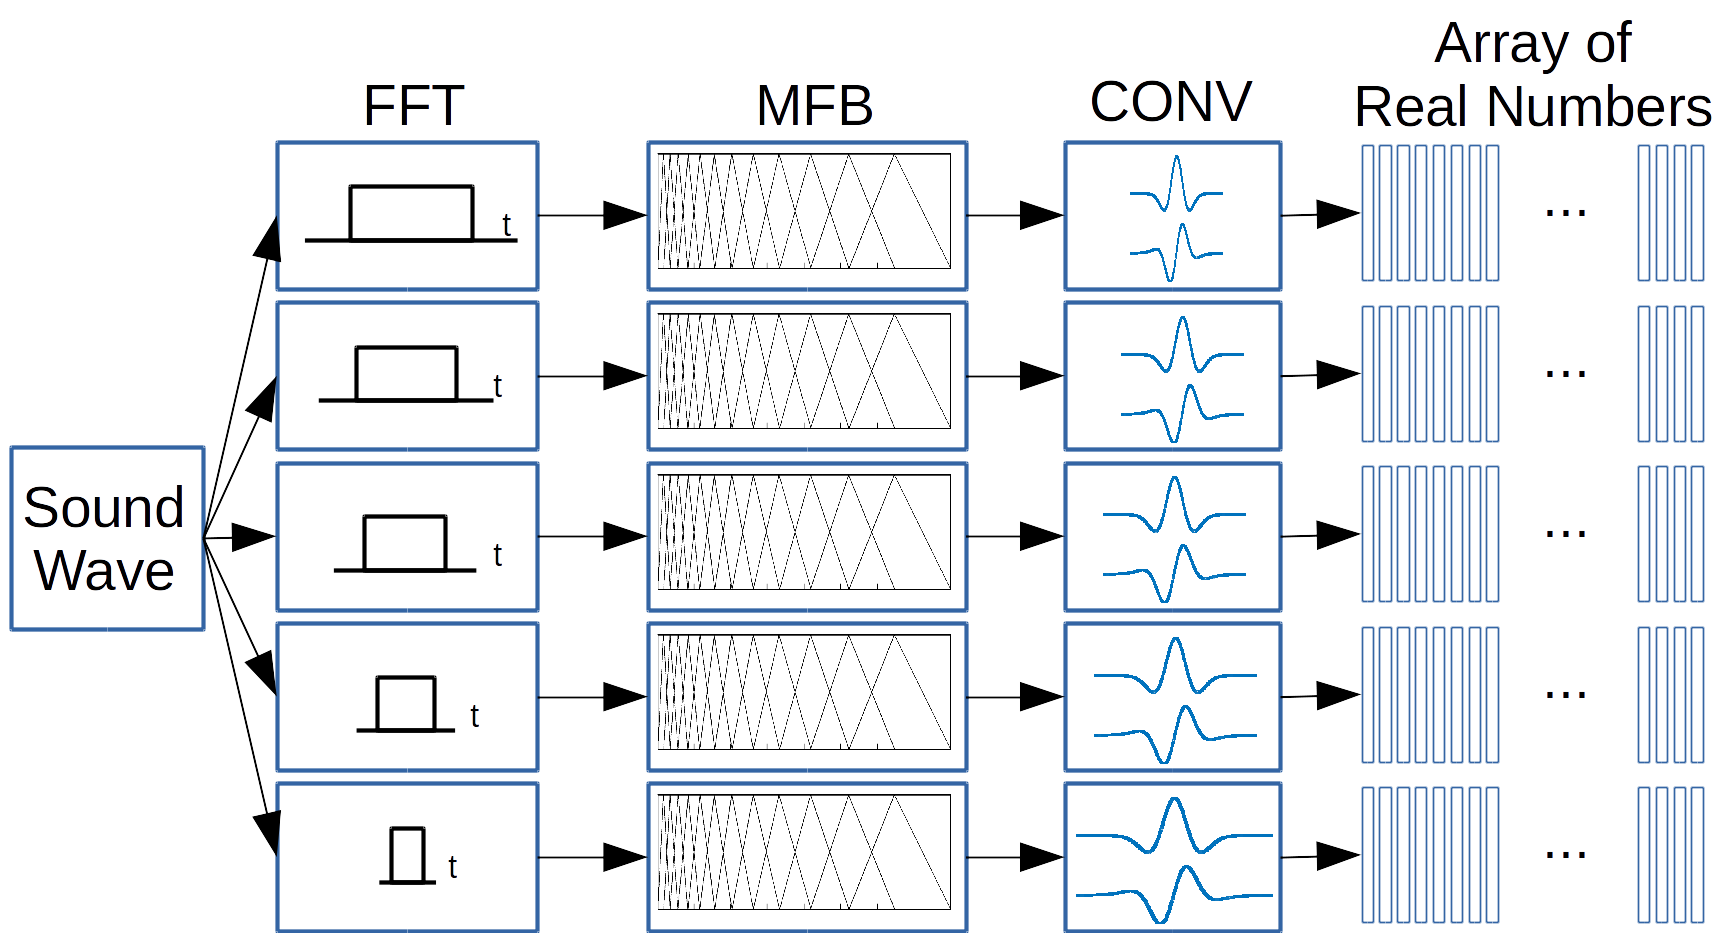
\includegraphics[width=0.8\textwidth]{MRSTSA.png}
    \caption{\reviewerfour{\glsfirst{mrstsa} algorithm. Sound waves are processed by \glspl{fft} with different time windows, then each spectrum is processed by
    a \glsfirst{mfb} and each resolution is convolved with a complex signal with a different coefficient. Finally, each filter coefficient
    is obtained computing the modulus from the convolution and then applying an automatic gain control.}}
    \label{fig:MRSTSA}
\end{figure}

We obtained the magnitude of each convolution and applied normalization to each time window
as a mean of automatic gain control in order to prioritize the information delivered by the
spectral configuration and not the absolute values delivered by the filters. 

By means of this constraint we account for the mechanical and chemical properties of hair cells in the mammalian inner ear
which constitute a transduction mechanism that appears to adapt to recent stimulus history in a way that can affect its gain
\cite{eatock_2000,holt_2000,le_goff_2005}. 
We decided to be conservative, not including
sound intensity dimension but just the shape of the filter responses.



~\\
\noindent{\underline{\textit{\glsfirst{el}}}}
~\\
~\\

The \gls{el} is responsible for generating \glspl{sdr} from the inputs delivered by the \gls{mrstsa} stage
described in the previous section and from the activation history in its own \glspl{cc}.

The \gls{el} simulates a patch of cortical tissue called \gls{cl}using an n-dimensional array of complex structures called \glspl{csom} that simulate \glspl{cc} in the brain.

Each \gls{cc} in the \gls{el} is connected to the \gls{mrstsa} below by means of afferent connections. It is also
connected to neighboring \glspl{cc}--including possibly itself--in the \gls{el} by means of lateral connections and
to \glspl{cc} from other \glspl{cl} above by means of apical connections. Such connection scheme is shown in Fig \ref{fig:EncoderColumnConnections}.

\begin{figure}[h!]
    \centering
    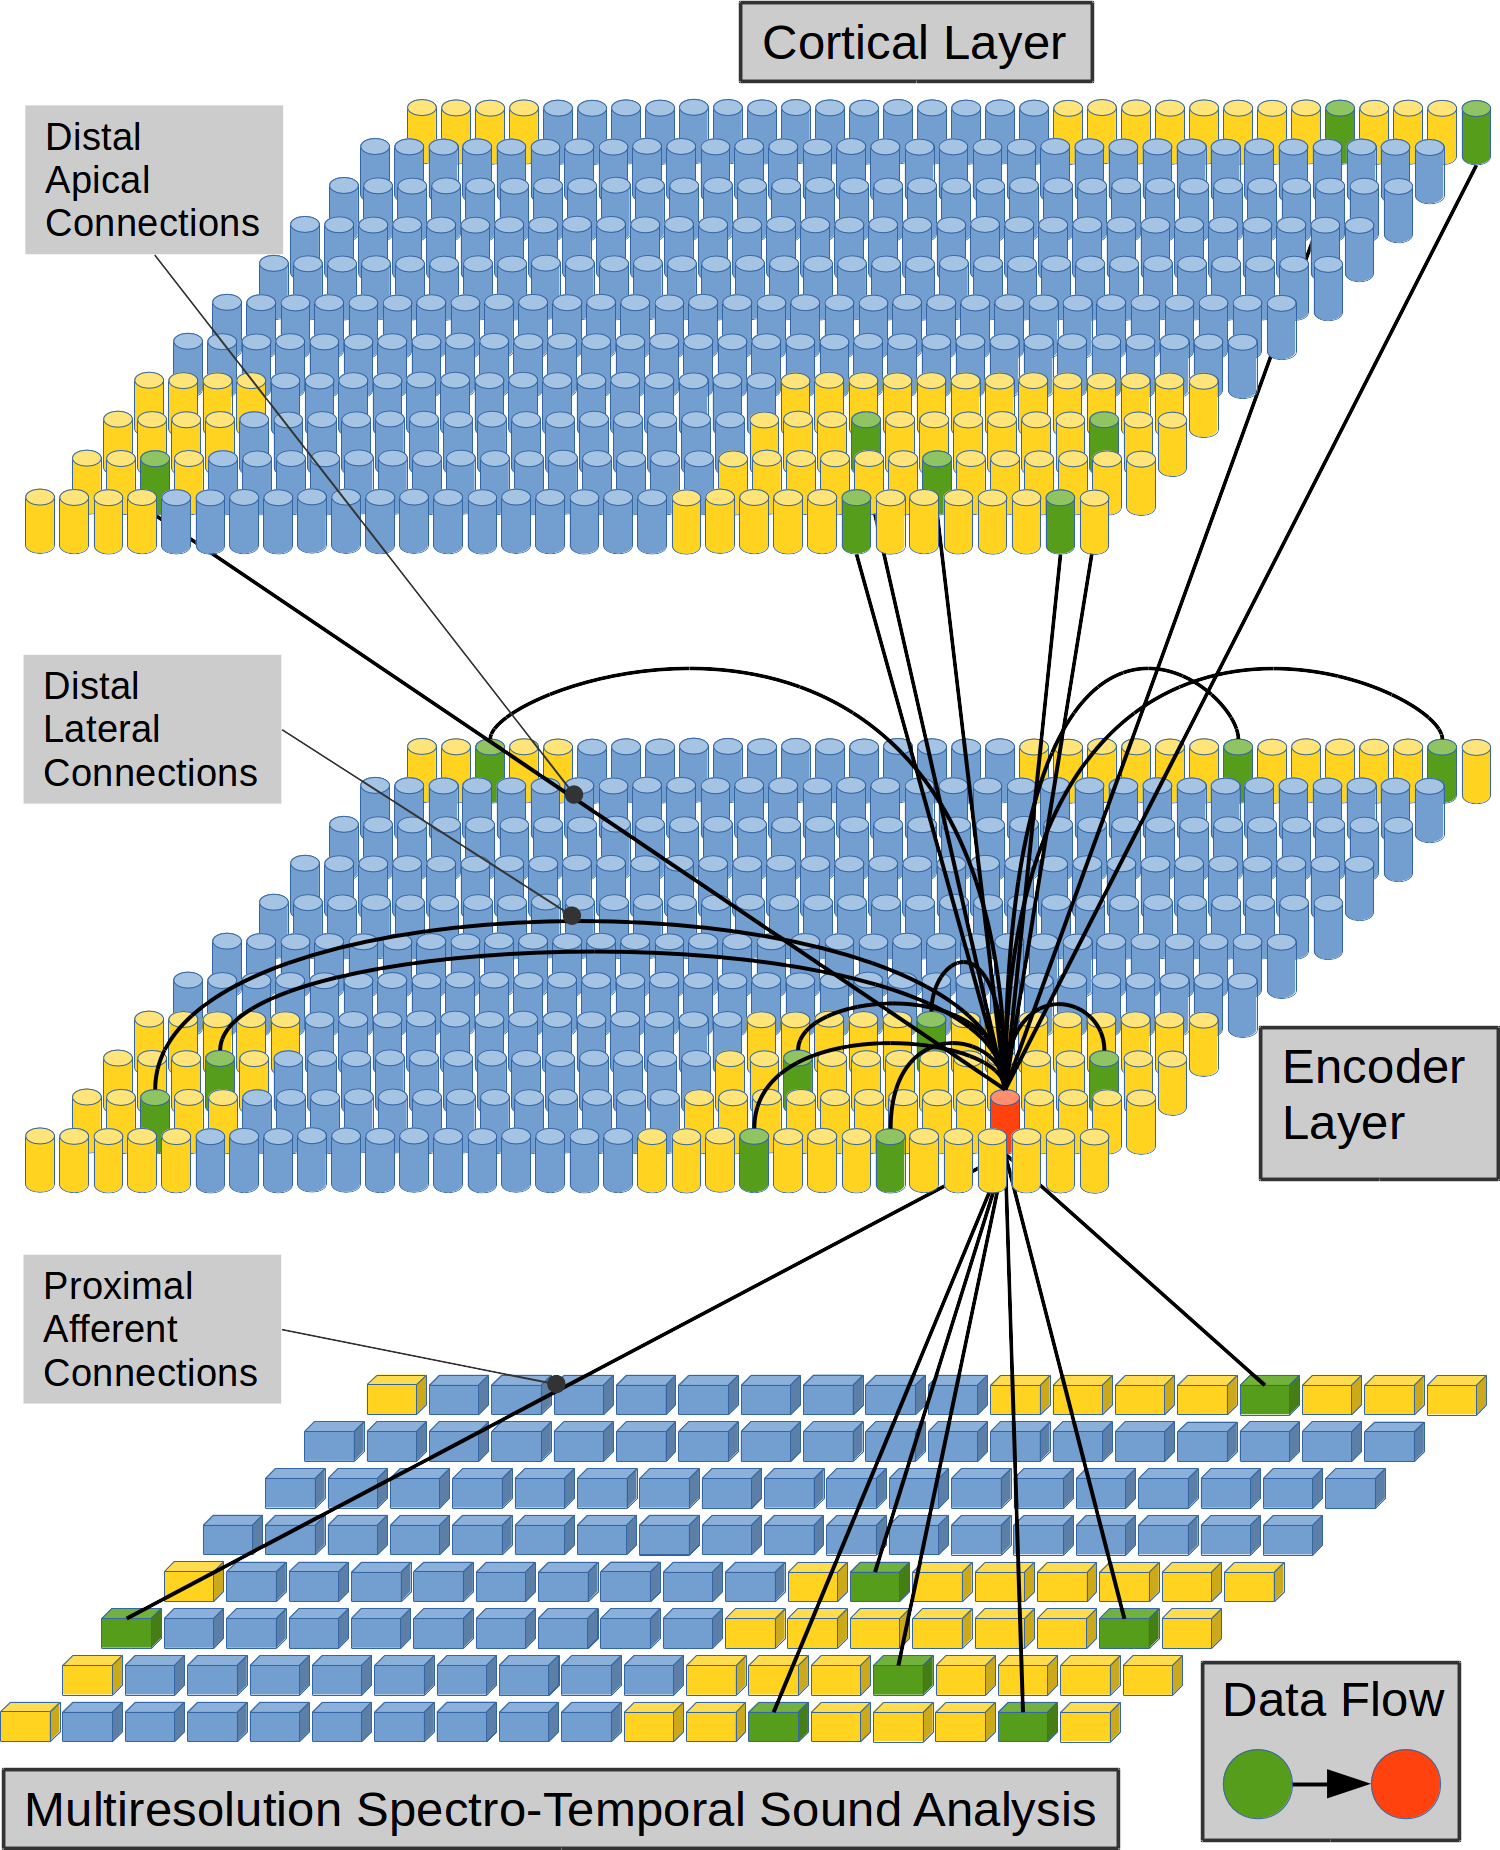
\includegraphics[width=0.6\textwidth]{EncoderColumnConnections.png}
    \caption{Connection scheme for a cortical column in the Encoder Layer.
	    Each cylinder in the \gls{el} and in the \gls{cl} represents a \gls{cc} in neural tissue.
	    Each prism in the \gls{mrstsa} represents a real valued variable.
	    This is a visualization of a \gls{cc} (in red) and its three receptive fields (in yellow).
	    The receptive field of a \gls{cc} is an array that defines a set of \glspl{cc}
	    with which such column could be connected.
	    The receptive field of a \gls{cc} on the \gls{mrstsa} determines an array of real valued variables
	    with which such column could be connected.
    A subset of \glspl{cc} in a receptive field (in green) represents the \glspl{cc} that are really
    connected with the \gls{cc} in red. A similar scenario could be described for the green prisms on
    the \gls{mrstsa}.
    The size, wrap-around property and percentage of established links (in green) inside a receptive field are tunable parameters for the model.
    In this work, only lateral connections have been implemented since in the current implementation there are no upper cortical layers from which
    to bring apical connections.}
    %Every neural unit in a \gls{cc} in the \gls{el} receives the same set of proximal connections from
    %the \gls{mrstsa}.
    %Such connections are modified following the statistical distribution from the \gls{mrstsa}
    %by means of the \gls{som} algorithm.}
    \label{fig:EncoderColumnConnections}
\end{figure}

\pagebreak


Both lateral and apical are feedback connections that constitute contextual information channels. 
These channels put the current afferent excitation under the context of previous activations.
Such connections damp the activity of some units allowing only the precise activations
of specific neural units in an afferently excited \gls{cc}.
Such precise activations match the sequential paradigms learned by the network.

Recent findings in neuroscience \cite{Marques2018} support the idea 
that feedback could potentially enhance visual representations in time and space
damping the activity of certain cells while allowing the activations  of others
which agree with their predictions.

In the present work we only implement lateral connections since
there are no upper layers 
from which to bring apical information in the present implementation.

Each cell unit in a \gls{cc} has two types of dendritic branches; proximal and distal.
Proximal and distal dendritic branches lead to proximal and distal connections in a cell unit respectively.
Proximal and distal connections produce different effects on a neural unit's plasticity and activation.
Neural units in the \gls{el} simulates pyramidal cells in cortical tissue in the brain.
Fig \ref{fig:PyramidalCell} shows the connectivity profile in such units. 

~\\
\noindent{\textit{Proximal dendritic connections}}
~\\
~\\

In reference to proximal connections in the \gls{el}, each neural unit in a \gls{cc} has the same set of
proximal connections to the \gls{mrstsa} \reviewerfour{(Fig \ref{fig:EncoderProximalConnections})}.
Such connections constitute a multidimensional space of real numbers.
In order to acquire the statistical distribution in such multidimensional real space we use
a multidimensional \gls{som} in each cortical column \reviewerfour{(Alg.~\ref{csom_proximal_synapses})}.

\begin{figure}[h!]
    \centering
    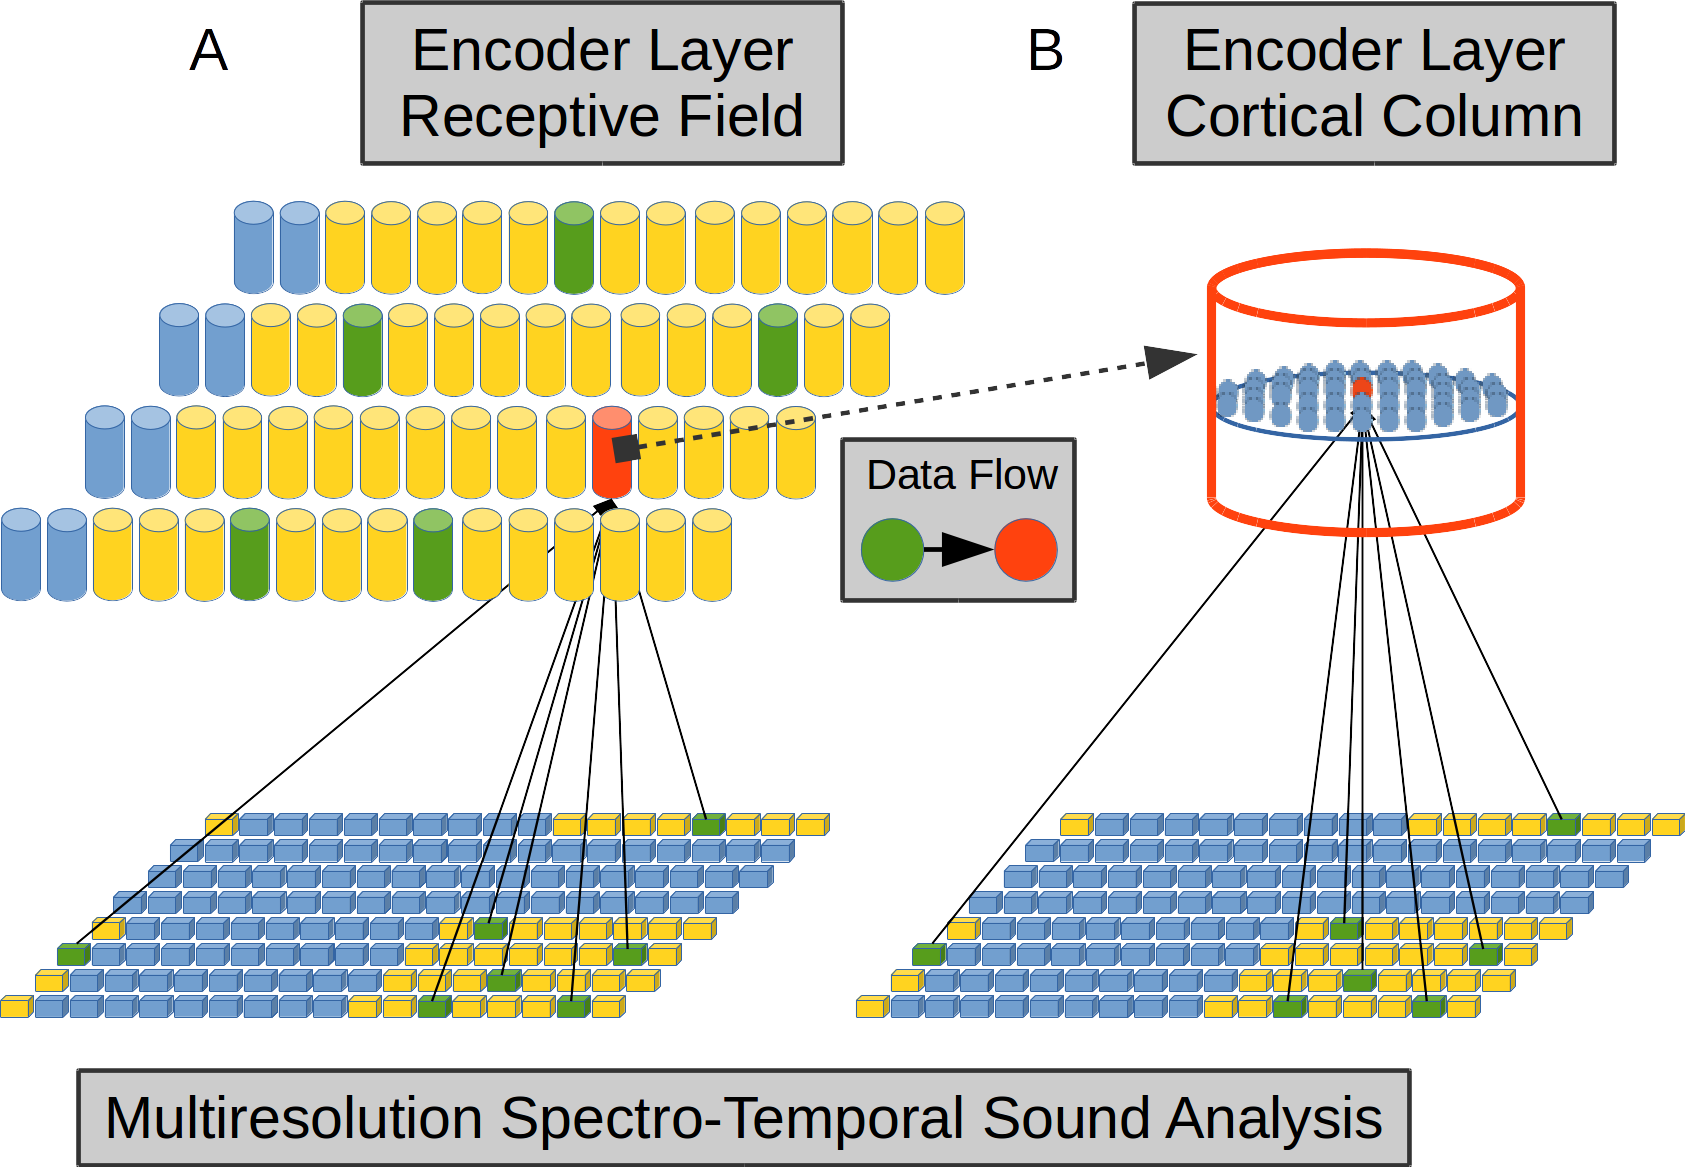
\includegraphics[width=0.8\textwidth]{EncoderProximalConnections.png}
    \caption{\reviewerfour{\glsfirst{el} proximal connections. Each \gls{cc} in the \gls{el}--exemplified here in red--has its receptive field over the \gls{mrstsa}--in yellow.
    (A) A set of \gls{mrstsa} components--in green inside the receptive field--is randomly chosen to be connected with such \gls{cc}.
    (B) Each neural unit in such \gls{cc} is connected with the same set of \gls{mrstsa} components.}}
    \label{fig:EncoderProximalConnections}
\end{figure}


\begin{algorithm}
	\caption{\reviewerfour{\texttt{Plasticity in Proximal Synapses}. \glsfirst{som} algorithm.}}
\label{csom_proximal_synapses}
\begin{algorithmic}[1]
	\STATE{given an \texttt{input} vector, find the nearest \texttt{unit} to such \texttt{input} vector in the input space}
	\STATE{move such \texttt{unit} towards the \texttt{input} vector in the input space (the magnitude of such movement depends on the learning rate)}
	\STATE{also move neighbor \texttt{units} to the nearest one towards the \texttt{input} vector (the magnitude of such movement depends on the learning rate and on a neighborhood measure over the topology of the network of units)}
\end{algorithmic}
\end{algorithm}

A \gls{som} is an unsupervised clustering algorithm which distributes a continuous multidimensional distribution
in a discrete multidimensional distribution of units \cite{Kohonen:1989:SAM:69371, kohonen_2082}.
In this way we ended up with an array of units of $m$ dimensions in which each unit
represents a set of vectors from the continuous distribution in an input space of $n$ dimensions.
Generally, $m < n$ in order to reduce the dimensionality in the discrete representation.
We added such restriction in our columnar algorithm.

In the \gls{som} algorithm, each input vector has to be completely determined.
In our case, several elements in the inputs from the \gls{mrstsa} could be null,
and considering such null inputs could inpair learning. 
Hence, each input vector could not have the information of each of its components available.
We incorporated a stochastic mechanism in the \gls{el} in order to deal with such situation.
We made each afferent connection to learn statistical boundaries from its corresponding input.
We establish a minimum-maximum margin in each proximal connection in the \gls{el}.
Such margin is consistent with the statistical distribution in the history of its corresponding input.
When an afferent input is undetermined, in a context in which some afferent inputs have
available information,
the \gls{el} chooses
the value in the undetermined input
%is chosen
randomly
between the boundaries learned for such input.

We call our implementation of the \gls{som} algorithm, \gls{ssom}.
The \gls{ssom} algorithm accounts for proximal lateral intra-column interaction, \gls{ltp} and
\gls{ltd}.
It also dissociates proximal dendritic inputs from distal dendrites, since
it modifies
proximal connections
%are modified
following the statistical distribution from the
\gls{mrstsa} independently of the units that fire in such \gls{cc}.
This independence in the plasticity of the proximal dendritic inputs
%uses
is supported by
the
%fact
property
found in cortical tissue by means of which there is dendritic plasticity
in the context of partial depolarization of the soma \cite{reiter_1998}--that is, without an \gls{ap}. % Citation needed here

The term \textit{static} comes from the fact that the patterns learned from proximal afferent
dendrites do not account for the contextual history in the dynamic evolution
of the algorithm.








~\\
\noindent{\textit{Distal dendritic connections}}
~\\
~\\

In terms of distal dendritic branches, each \gls{cc} in the \gls{el} is connected to other \glspl{cc}--in green in Fig \ref{fig:EncoderColumnConnections}--by means of such
branches inside the receptive fields--in yellow in Fig. \ref{fig:EncoderColumnConnections}--from the same \gls{el} and from another \gls{cl}
above.
Each link between the red \gls{cc} and a green \gls{cc}--Fig. \ref{fig:DistalDendrites} A--
symbolizes the fact that each cell unit in
the red \gls{cc} is linked with a different subset of cell units in the green \gls{cc}--Fig. \ref{fig:DistalDendrites} B.

\begin{figure}[h!]
    \centering
    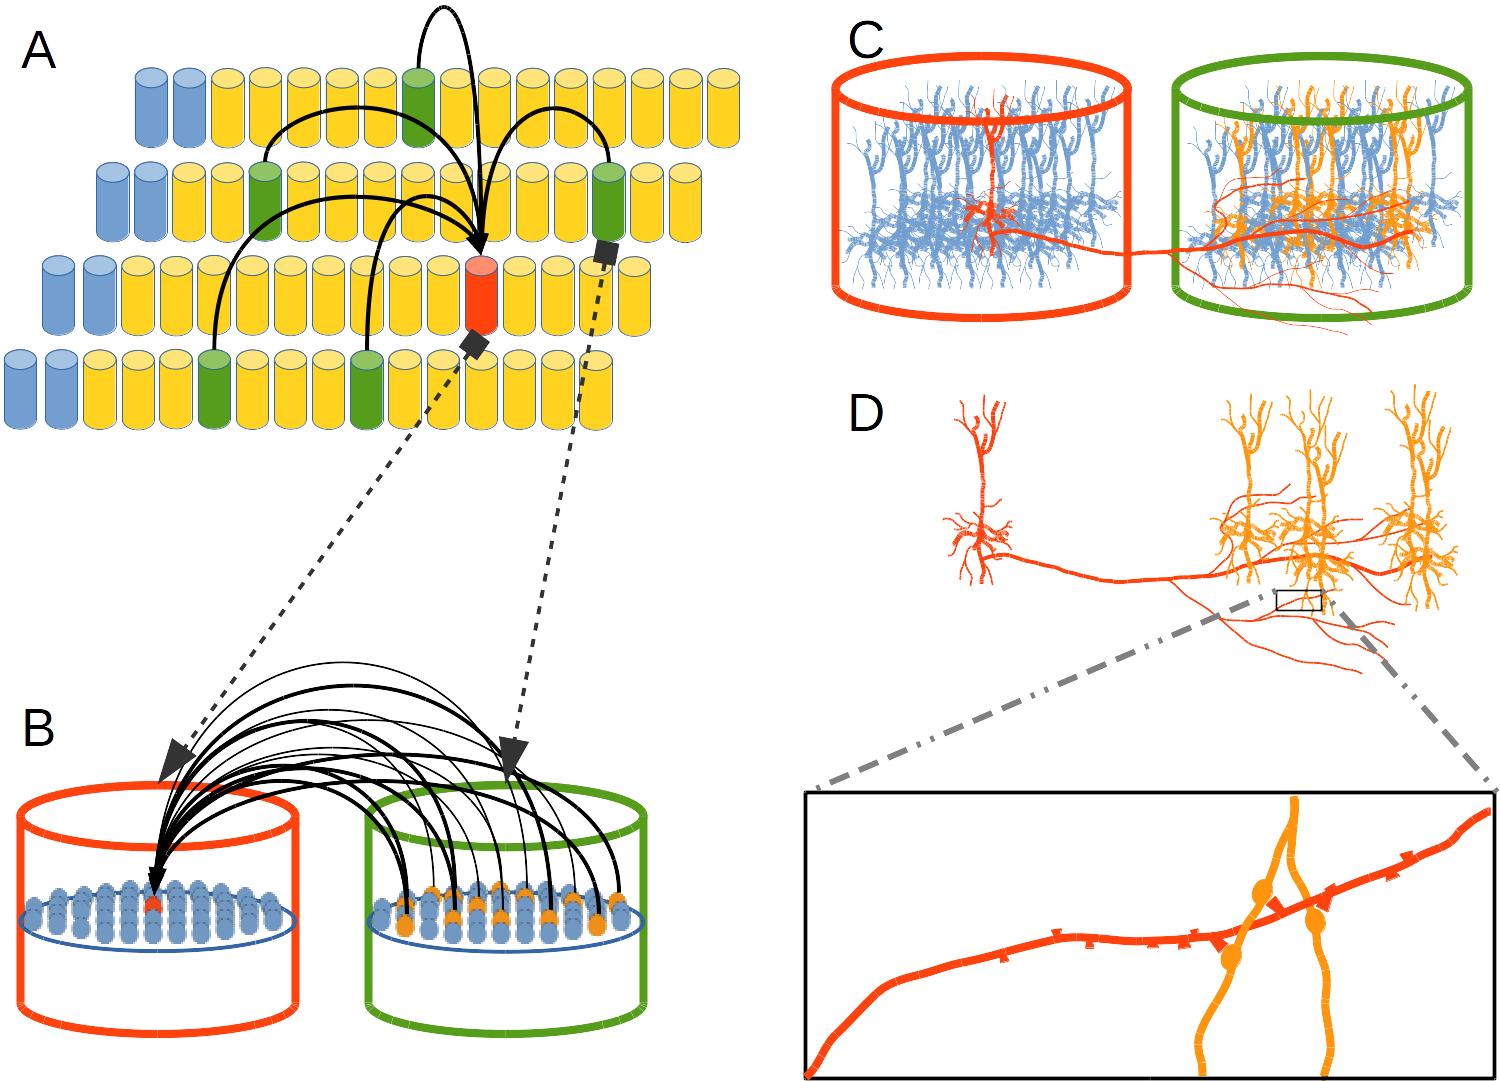
\includegraphics[width=0.9\textwidth]{DistalDendrites.png}
    \caption{Distal dendrite connections. (A) Distal dendritic branches from neighboring \glspl{cc} inside the receptive field
    of a \gls{cc} in the \gls{el}. A distal dendritic branch between the red \gls{cc} and a
    green \gls{cc} means that every neural unit in the red \gls{cc} is linked with a different
    subset of neural units in the green \gls{cc} by means of potential connections.
    (B) Potential connections in a dendritic branch which link a neural unit in the red \gls{cc}
    with a subset of neural units in a green \gls{cc}. The subset of potential connections comes from a percentage of neural units
    inside the green \gls{cc}. Such percentage is a tunable parameter for the \gls{cc}.
    (C) A distal dendritic branch between a pyramidal cell in a \gls{cc} and a 
    sub-set of pyramidal cells in a neighboring \gls{cc} inside its receptive field
    in the \gls{el}.
    (D) Physical proximity of a dendritic branch from the red cell to axonal branches from yellow cells constitutes potential connections
    which could prosper becoming in established synapses depending on the sequential activity among cells.}
    \label{fig:DistalDendrites}
\end{figure}

\pagebreak

Such links in Fig \ref{fig:DistalDendrites} A, represent dendritic branches in neural tissue and
we call
each connection in Fig. \ref{fig:DistalDendrites} B,
%is called
potential connection.
%and
Potential connections represent synapses in the dendritic branch.
A cell unit inside the red \gls{cc} ends up with as many dendritic branches as green \glspl{cc} inside its receptive field (Fig \ref{fig:DistalDendrites} A.)

The term \emph{potential connection} is used, because it describes a pair of neural units linked by its physical location and dendritic and axonal disposition in cortical tissue (Fig. \ref{fig:DistalDendrites} C). However, an effective connectivity between such neurons will depend upon their sequential pattern of activation which will establish developed synapses between them. If two neural units--a red one and a yellow one in Fig. \ref{fig:DistalDendrites} D--are linked by means of a distal potential connection--produced by a synapse between a distal dendritic branch from the red one and an axonal branch from the yellow one--such connection will grow only if there is a sequential activation of the red cell after an activation of the yellow cell, in two consecutive time steps. If such phenomenon does not repeat itself over time, such synapse will decrease its strength with respect to other synapses in the dendritic branch in the red cell in Fig. \ref{fig:DistalDendrites} D. A simultaneous activation in both neural units--the red one and the yellow one in Fig. \ref{fig:DistalDendrites} D--will decrease the strength in such potential connection.

We implemented distal dendritic synaptic plasticity mechanisms by means of an algorithm called \gls{dsom} \reviewerfour{(Alg. \ref{csom_distal_synapses})}.
The learning mechanisms implemented on such algorithm simulate neurophysiological phenomena
such as \gls{stdp}, and homeostatic regulation plasticity in the synaptic strength regulation in
distal dendritic branches.

\begin{algorithm}
	\caption{\reviewerfour{\texttt{Plasticity in Distal Synapses}. This algorithm accounts for \glsfirst{stdp} and homeostatic regulation phenomenon in distal dendritic synapses.}}
\label{csom_distal_synapses}
\begin{algorithmic}[1]
	\FOR{every active \texttt{unit} in this cortical \texttt{column}}
		\FOR{every \texttt{dendrite} in this active \texttt{unit}}
			\STATE {increment all the \texttt{synapses}--in this dendrite--potentially connected to \texttt{units} which were active in the last time step}
		\ENDFOR
	\ENDFOR
	\FOR{every active \texttt{unit} in this cortical \texttt{column}}
		\FOR{every \texttt{dendrite} in this active \texttt{unit}}
			\STATE {decrement all the \texttt{synapses}--in this dendrite--potentially connected to \texttt{units} which are active in this time step}
		\ENDFOR
	\ENDFOR
	\IF{updated \texttt{step} reaches certain value}
		\FOR{every \texttt{unit} in this cortical \texttt{column}}
			\FOR{every \texttt{dendrite} in this \texttt{unit}}
				\IF{the sum of the \texttt{synapses} in this \texttt{dendrite} is greater than one}
					\STATE {normalize all \texttt{synapses} in this \texttt{dendrite}}
				\ENDIF
			\ENDFOR
		\ENDFOR
		\STATE{updated \texttt{step} = 0}
	\ENDIF
	\STATE{updated \texttt{step}++} 
\end{algorithmic}
\end{algorithm}

\reviewerfour{Basically, Alg.~\ref{csom_distal_synapses} updates all distal axonal-dendritic synapses, incrementing  them always that pre and post-synaptic neural units become active in consecutive time steps, and decrementing them when they become active at the same time step. Occasionally, all the synaptic weights belonging to the same dendrite are normalized every certain number of time steps. This normalization is repeated for all neural units and for all dendritic branches in each neural unit whose sum of synaptic weights is beyond unity}.







~\\
\noindent{\textit{Activation rules in a \gls{cc}}}
~\\
~\\

Finally, in reference to the activation rules of neural units inside a \gls{cc} in the \gls{el},
first a group of cell units in a \gls{cc} is partially depolarized 
by distal connections among such neural units and cell units activated in the
previous time step in the \gls{el}--Fig. \ref{fig:Activation} A.
That is, neural units activated in time step $t=0$ in the \gls{el}, will partially depolarize
a set of neural units in time step $t=1$ in such \gls{cc}, by means of distal--lateral and apical--
dendritic branch synapses established by learning in the \gls{dsom} algorithm.

Second, afferent proximal connections from \gls{mrstsa} will tend to depolarize
certain clusters of units in such \gls{cc} in time step $t=1$--Fig. \ref{fig:Activation} B.
The tentative depolarization is produced by the inputs from the \gls{mrstsa} with
proximal synapses established by learning in the \gls{ssom} algorithm. 
Such group of neural units are randomly chosen from a discrete distribution
whose probabilities are established by the state of excitation in afferent inputs.

If a sufficient number of partially depolarized units are in the set of
afferently excited units, such partially depolarized units
will fire previously in the group--Fig. \ref{fig:Activation} B left.
Those units--which fire before--prevent neighboring units in the excited clusters from firing,
hyperpolarizing them by means of lateral inhibitory connections in the column.

\begin{figure}[h!]
    \centering
    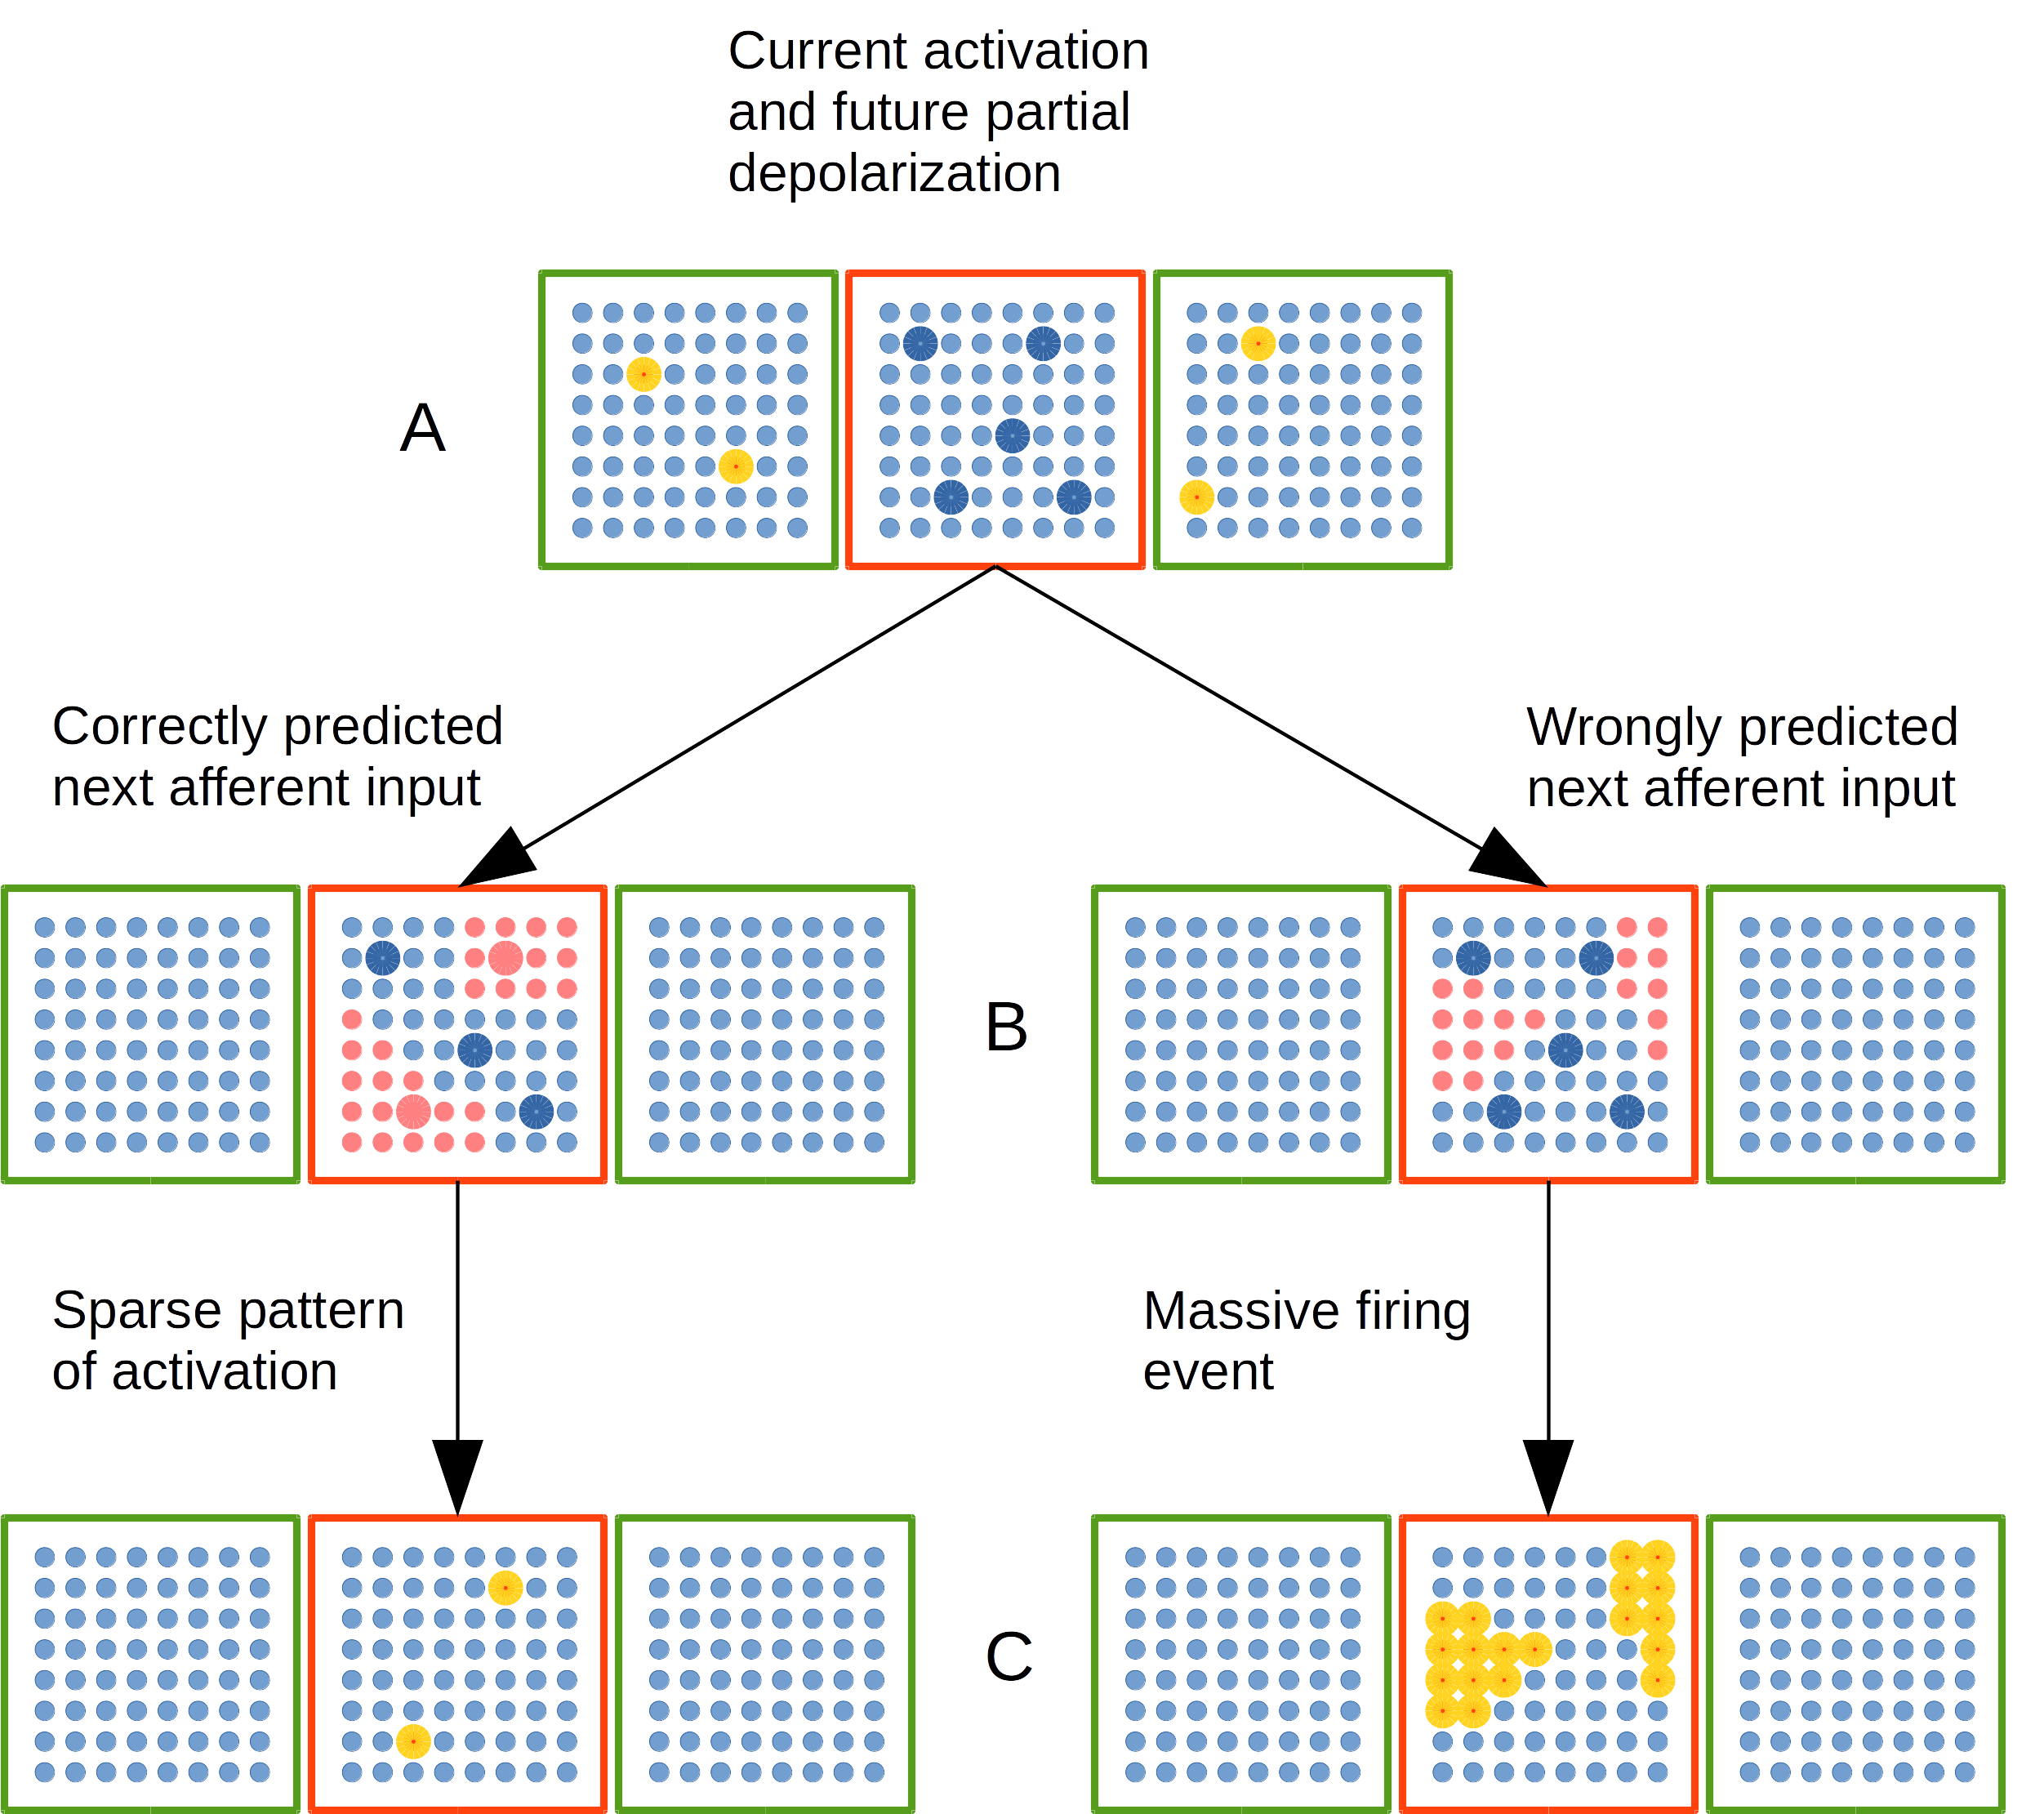
\includegraphics[width=0.7\textwidth]{Activation.png}
    \caption{Dynamic cellular activation in a \gls{cc} in the \gls{el}.
    A red cortical column is linked with two green cortical columns by means of distal dendrites.
    (A) Cellular activation in green \glspl{cc}--highlighted yellow cells--puts neural units
    in red \gls{cc} in a partially depolarized--predictive state highlighted in blue.
    (B) Cluster of neural cells activated by afferent inputs.
    Left: A substantial amount of partially depolarized cells are in the afferently excited cellular clusters.
    Right: There is no substantial amount of partially depolarized cells inside afferently excited cellular clusters.
    (C) \gls{cc} with active cellular units highlighted in yellow.
    Left: Sparse pattern of cellular activation.
    Right: Massive pattern of activation.}
    \label{fig:Activation}
\end{figure}

\pagebreak

Partial depolarization states put cell units in a predictive state generated by
the activations produced in the \gls{el} in previous time steps.
That is, lateral and apical activation in previous time steps constitute a context in which
current afferent inputs are received.

From the group of units that tend to be depolarized by current afferent inputs from the \gls{mrstsa},
only a reduced sub-set of those units are likely to fire in the previous contextual firing history
in the \gls{el}--Fig. \ref{fig:Activation} C left.

In case there is no context, that is, \reviewertwo{if not enough number of the units normally depolarized by afferent inputs
are partially depolarized by previous--lateral and apical--activations}--Fig. \ref{fig:Activation} B right--,
all units in the afferent excited clusters will be active, covering more hypotheses for next inputs--Fig. \ref{fig:Activation} C right.

\reviewerfour{Such activation mechanism is depicted in Alg. \ref{csom_activation}. In Alg. \ref{csom_activation} (Part 1) a ranking is established among neural units--inside a \gls{cc}--in terms of its afferent excitability, given the afferent inputs (lines 1 and 2). The \emph{number of afferently excited units}  refers to the maximum number of  units that can be activated by the afferent input in a \gls{cc} and \emph{minimum number of active units} refers to the number of units that will be active in a \gls{cc} if a \gls{sdr} is achieved as a result of optimal prediction (lines 3 and 4 respectively)}.

\begin{algorithm}
	\caption{\reviewerfour{\texttt{Units activation (Part 1)}. This algorithm establishes the activation rules in a \gls{csom} object.}}
\label{csom_activation}
\begin{algorithmic}[1]
	\STATE{\texttt{distances} = given an \texttt{input} vector find the euclidean distance each \texttt{unit} has to such \texttt{input} in the input space from proximal afferent synapses}

	\STATE {\texttt{ranking} = sort indexes from the smallest to the largest \texttt{distances}}

	\STATE{number of afferently excited units = proximal activation percentage*number of units}

	\STATE{minimum number of active units = (1-sparsity)*number of units}

	\IF{randomness is disabled}
		\STATE {excited \texttt{units} = gets the first \emph{number of afferently excited units} elements from \texttt{ranking}}
	\ELSE
		\STATE {excited \texttt{units} = gets \emph{number of afferently excited units} random indexes from \texttt{distances} with probabilities determined by the relative reciprocal of the \texttt{distances} element values}
	\ENDIF

	\FOR{\texttt{unit} = 0 \TO \texttt{unit} = number of units }
		\STATE{auxiliary = 0}
		\FOR{\texttt{dendrite} = 0 \TO \texttt{dendrite} = number of distal dendrites }
			\STATE{\texttt{dendrite} accumulator = 0}
			\FOR{\texttt{active unit} = 0 \TO \texttt{active unit} = number of linked active units}
				\STATE{potential \texttt{index} = find the first coincident index in potential \texttt{connections[dendrite][unit]} with linking \texttt{units[dendrite][active unit]}}
				\IF{there exist coincidence}
					\STATE {\texttt{dendrite} accumulator += dynamic \texttt{synapses[dendrite][unit][\textnormal{potential} index]}}
				\ENDIF
			\ENDFOR
			\IF{\texttt{dendrite} accumulator $>$ 100*DISTAL\_SYNAPTIC\_THRESHOLD}
				\STATE {auxiliary++}
			\ENDIF
		\ENDFOR
		\STATE{total \texttt{responses[unit]} += auxiliary}
	\ENDFOR
	\STATE{updated \texttt{distances} = element wise quotient between \texttt{distances} and total \texttt{responses}}
	\STATE {updated \texttt{ranking} = sort indexes from the smallest to the largest updated \texttt{distances}}

\end{algorithmic}
\end{algorithm}

\reviewerfour{If randomness is enabled, \emph{number of afferently excited units} units is chosen at random by means of a discrete distribution whose probabilities are the afferent excitation of each unit. If randomness is disabled, \emph{number of afferently excited units} first units are chosen from the ranking of afferently excited units (lines 5 to 9)}.

\reviewerfour{From line 10 to 25 each neural unit accumulates distal--lateral and apical--excitation in order to determine its partial depolarization from units which were active in the previous time step. For each neural unit in a \gls{cc}, for each distal dendrite in such unit and for each active unit in such distal dendrite the algorithm looks for coincidences between some potential connection in such distal dendrite in the neural unit and the active unit in such distal dendrite. That is, in line 15, the algorithm asks if there is coincidence between some potential connection in this distal dendrite inside the unit and the neural unit activated in the previous time step in the \gls{cc} linked by such distal dendrite. If there is coincidence, the value of the synaptic weight in such potential connection is accumulated in a dendrite accumulator. After all active units are examined for this dendrite, if the dendrite accumulator is greater than certain threshold, such dendrite is considered active and the total response of the unit is incremented in one}.

\reviewerfour{Each neural unit ends up with an excitation value due to its distal dendrites. The unit distances vector is element- wise divided by distal dendritic excitations vector to get the updated distances and an updated ranking of the units (lines 26 and 27). In this way, units with more distal excitation will decrease its distance more and will be put in a more favorable place in the ranking in order to be activated}.

\reviewerfour{In Alg. \ref{csom_activation} (Part 2) the minimum updated distance is found in the group of afferently excited units. Then, a set of units--inside the group of afferently excited units--is identified which have such minimum updated distance. While the number of identified units is less than \emph{minimum number of active units}, the next   minimum updated distance is found in the group of afferently excited units and a new set of units--inside the group of afferently excited units--is identified which have such next minimum updated distance. This new set is added to the previous one until the number of units in this accumulative set is greater than or equal to the minimum number of active units}.

\begin{algorithm}
\ContinuedFloat
\caption{\reviewerfour{\texttt{Units activation (Part 2)}. This algorithm establishes the activation rules in a \gls{csom} object.}}
\label{csom_activation}
\begin{algorithmic}[1]
	\STATE{new \texttt{distances} = get the updated \texttt{distances} elements whose indexes are in excited \texttt{units}}
	\STATE{new minimum \texttt{distance} = get the minimum element from new \texttt{distances}}
	\STATE{minimum \texttt{indexes} = get indexes from updated \texttt{distances} vector whose values are equal to new minimum \texttt{distance}}
	\STATE{apt to be \texttt{active} = get the coincident indexes between excited \texttt{units} and minimum \texttt{indexes}}
	\STATE{erase from new \texttt{distances} vector, all the elements whose value is equal to new minimum \texttt{distance}}

	\WHILE{number of elements in apt to be \texttt{active} vector $<$ \emph{minimum number of active units} and new \texttt{distances} has at least one element}
		\STATE{new minimum \texttt{distance} = get the minimum element from new \texttt{distances}}
		\STATE{minimum \texttt{indexes} = get indexes from updated \texttt{distances} vector whose values are equal to new minimum \texttt{distances}}
		\STATE{partial apt to be \texttt{active} = get the coincident indexes between excited \texttt{units} and minimum \texttt{indexes}}
		\STATE{incorporate partial apt to be \texttt{active} elements into apt to be \texttt{active} vector}
		\STATE{erase from new \texttt{distances} vector, all the elements whose value is equal to new minimum \texttt{distance}}
	\ENDWHILE

	\IF{ENABLE\_RANDOM\_BEHAVIOUR}
		\STATE {shuffle apt to be \texttt{active} vector}
	\ENDIF

	\FOR{\texttt{number} = 0 \TO \texttt{number} = number of apt to be \texttt{active} elements }
		\STATE {incorporate to \texttt{output} the excited \texttt{units[\textnormal{apt to be} active[number]]}}
	\ENDFOR

	\RETURN \texttt{output}
\end{algorithmic}
\end{algorithm}

\reviewerfour{The functional result of Alg. \ref{csom_activation} is that there must be a sufficient amount of--partially and previously depolarized--neural units inside the afferently activated cluster of units in order to get a \gls{sdr} pattern of activation. Otherwise, the \gls{cc} will end up with a massive activation pattern, a \glsfirst{mfe} in which more than a \emph{minimum number of active units} will be active. In the case of the occurrence of a \gls{mfe}, the synaptic plasticity is modulated in order to form stronger synapses of those neural units activated during such event}.

Each neural unit in a \gls{cc} establishes its state of partial depolarization based on the contribution from
distal dendritic branches from lateral and apical connections.
A dendritic branch will contribute to the partial depolarization of the soma in such cell only if such
dendritic branch exceeds an activation threshold by means of the contribution from its individual synapses
in the context of the patterns of activation in the previous time step.

This mechanism has compelling sequential properties \cite{hawkins_2016},
which have already been applied in the classification of artificially generated sequential data \cite{cui_2016}.
We apply such mechanism in the \gls{dsom} algorithm by adding the contribution of synapses--in a dendritic branch--whose connections
are linked with cells that were active in the previous time step in the \gls{el}.
















\subsubsection*{Implementation}
\label{model-implementation}


~\\
\noindent{\underline{\textit{\gls{mrstsa}}}}
~\\
~\\

We apply \gls{fft} to the audio files with a sample period of 8 milliseconds.
We use the FFTW package \cite{FFTW05, fftw}
with time windows of 8, 16, 32, 64 and 128 milliseconds in order to obtain
a multiresolution power spectral analysis of the signal.
%We then applied 
In addition, we apply the Mel Filter-Bank technique with 128 filters to each
spectral resolution and convolve such filters along their tonotopic axis.
For the convolution, we use a multiresolution complex function whose real part
is a Mexican hat function and its imaginary part is the corresponding Mexican hat Hilbert transformation.
%-Fig. \ref{fig:Multi}.

%\begin{figure}[h!]
    %\centering
    %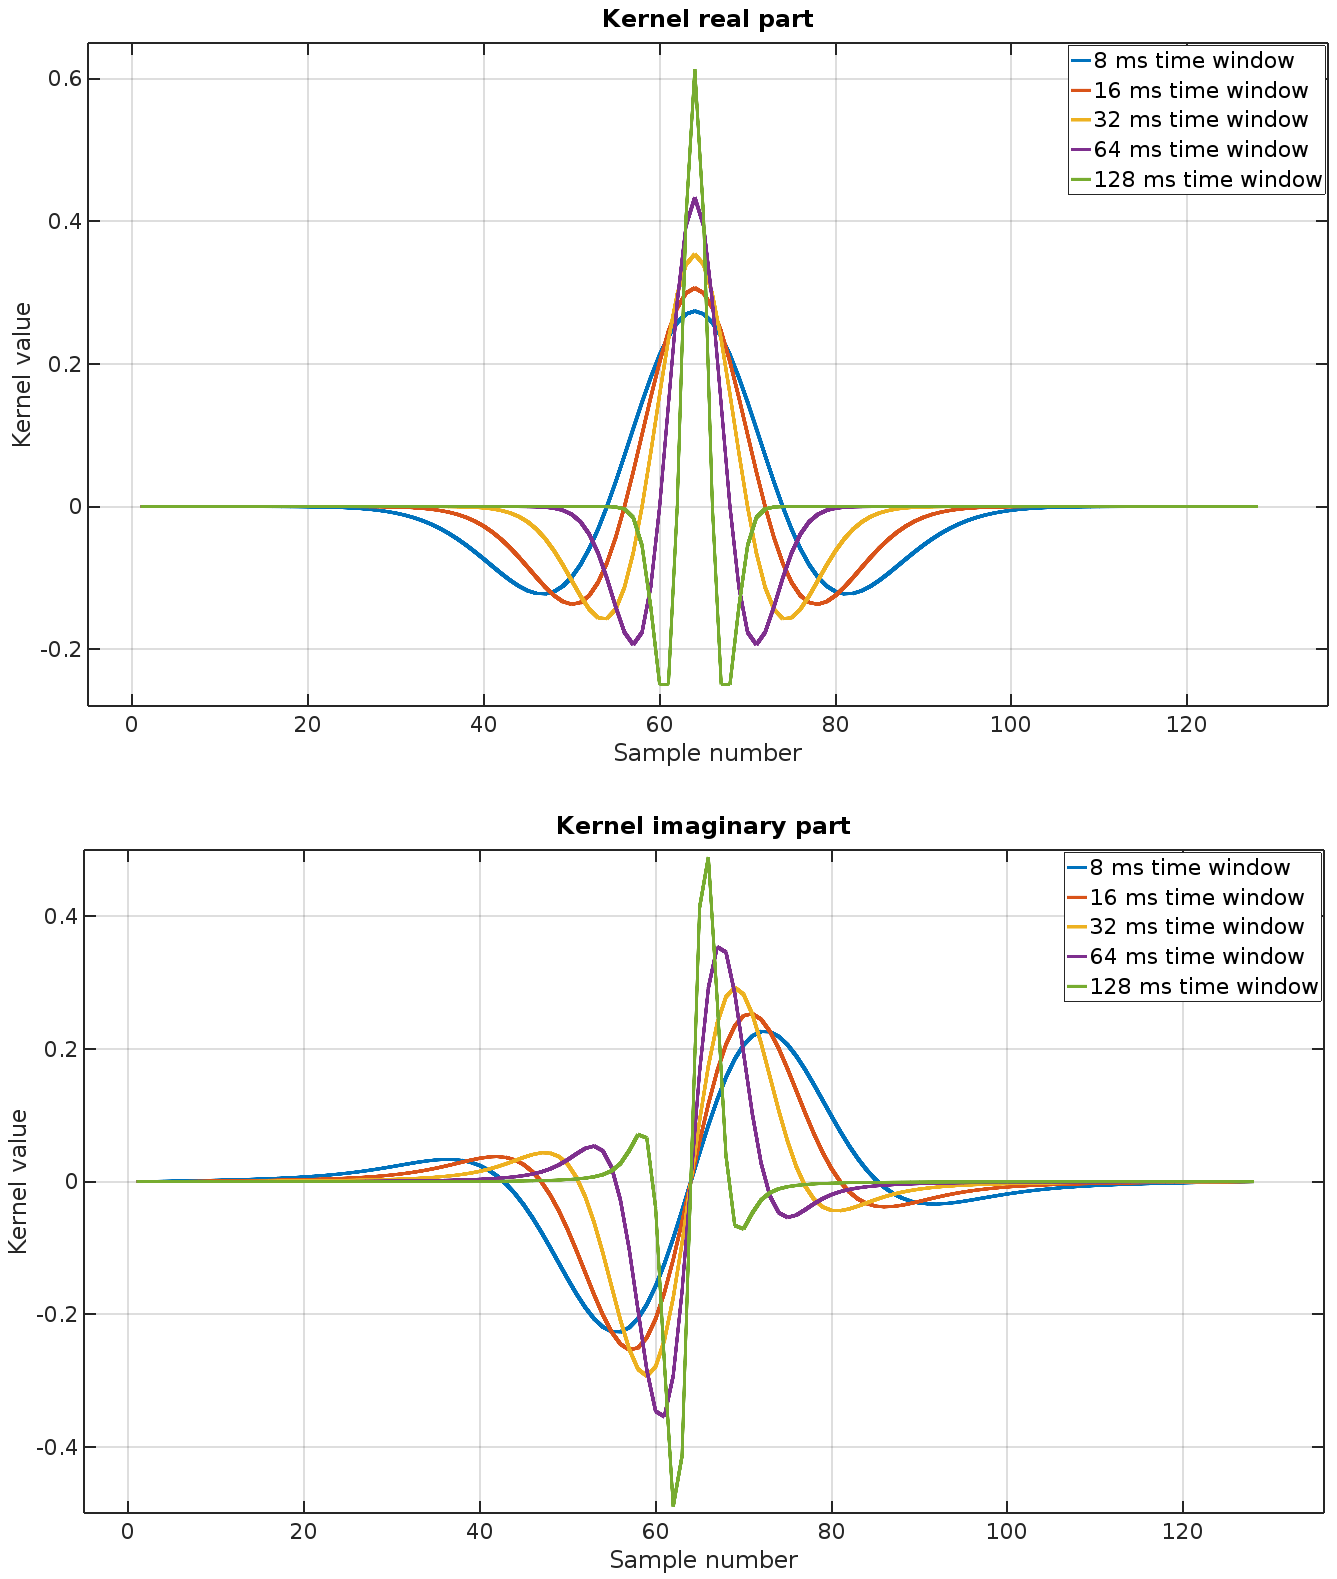
\includegraphics[width=0.7\textwidth]{Multi.png}
    %\caption{Multiresolution complex kernels. Such kernels are convolved with Mel Filter Bank outputs along their tonotopic axis.
	    %Each kernel has a different coefficient
    %and is convolved with its corresponding power spectral resolution.
    %The function coefficients are 10 for 8 ms time window, 8 for 16 ms time window, 6 for 32 ms time window, 4 for 64 ms time window
    %and 2 for 128 ms time window.}
    %\label{fig:Multi}
%\end{figure}

The function coefficients are 10 for the 8 ms time window, 8 for the 16 ms time window, 6 for the 32 ms time window, 4 for the 64 ms time window
and 2 for the 128 ms time window. We then compute the magnitude from the convolution and normalize in each time step.
By means of this procedure we obtain from the audio file a multiresolution spectro-temporal response composed by
an array of 128 columns--one column per filter--and 5 rows--one row per resolution--with real numbers which range from
0 to 1, for each time step.









~\\
\noindent{\underline{\textit{\gls{el}}}}
~\\
~\\

We implement an \gls{el} with 225 \glspl{csom} arranged in a two-dimensional
array of 15 by 15 \glspl{cc}. Each \gls{cc} is automatically distributed using individual locations along its afferent inputs in a uniform way.
Each \gls{cc} receives afferent information by means of
two-dimensional afferent receptive fields of 5 by 227 filters centered at individual locations over the \gls{mrstsa}.
We enable the wraparound property in order to make each receptive field span the entire
\gls{mrstsa} array.
We also instruct each column to receive only 31 inputs, which is a minor percentage of such
receptive field.
Individual afferent inputs for each \gls{cc} are chosen randomly in the \gls{el} initialization. 

For this model instance we implement only distal lateral dendritic branches since there are
no more \glspl{cl} from which to bring information through apical dendritic branches.
We configure each \gls{cc} to have a lateral receptive field with 9 by 9 neighboring \glspl{cc}
and to receive information from 72 of the 81 \glspl{cc} in the receptive field--a 90\% of the receptive field.

Each \gls{cc} is composed of a two-dimensional array with 15 by 15 (225) neural units and
each unit in a column could be potentially connected with only 6 neural units from each linked neighboring column. 
That is, each neural unit in a \gls{cc} ends up with 72 lateral dendritic branches with 6 potential connections each
(432 distal potential synapses per cellular unit).
Such potential synapses are randomly chosen for each neural cell and for each dendritic branch in the cell during the Encoder initialization procedure.
The \gls{el} consists of 50625 cellular units with 1569375 proximal synapses and 21870000 distal synapses.
\reviewerfour{Such specifications state the number of free parameters of the model, but it is important to highlight that distal synapses represent
potential connections from which only a small percentage has a significant synaptic weight as to be considered as an established connection.
Weak synapses are periodically pruned by means of homeostatic processes in the network leaving distal dendrites with a sparse connectivity in the receptive fields.
Typical sparseness in such connectivity matrices could exceed the 90\%.}

We train the \gls{el} using a 500 word corpora generated by the procedure described in section \nameref{CorpGen}.
The training procedure consists of 4 stages and for each stage the \gls{el} receives the same corpus 4 times.

During each learning stage, certain parameters--such as the learning rates in proximal and distal synapses and the lateral
intra-column interaction--are exponentially and progressively decreased from an initial value, which also decreases
for each successive stage.
An additional stage is executed with the learning parameters fixed.

The sparsity in the activation for each \gls{cc} is 99\% (just 2 neural units out of 225 could be active for normal activation events).
On the other hand, the afferent excitation affects 10\% of the units inside the clusters in each \gls{cc}
(22 neural units, which could be activated in case of a \gls{mfe}; Fig. \ref{fig:Activation}).









~\\
\noindent{\underline{\textit{\gls{svm} Classification}}}
~\\
~\\

%% For figure citations, please use "Fig" instead of "Figure".
%Nulla mi mi, Fig~\ref{fig1} venenatis sed ipsum varius, volutpat euismod diam. Proin rutrum vel massa non gravida. Quisque tempor sem et dignissim rutrum. Lorem ipsum dolor sit amet, consectetur adipiscing elit. Morbi at justo vitae nulla elementum commodo eu id massa. In vitae diam ac augue semper tincidunt eu ut eros. Fusce fringilla erat porttitor lectus cursus, \nameref{S1_Video} vel sagittis arcu lobortis. Aliquam in enim semper, aliquam massa id, cursus neque. Praesent faucibus semper libero.

%% Place figure captions after the first paragraph in which they are cited.
%\begin{figure}[!h]
%\caption{{\bf Bold the figure title.}
%Figure caption text here, please use this space for the figure panel descriptions instead of using subfigure commands. A: Lorem ipsum dolor sit amet. B: Consectetur adipiscing elit.}
%\label{fig1}
%\end{figure}

We use supervision by means of the \gls{svm} classification
method, receiving the outputs from each algorithm \cite{CC01a, libsvm}. We do this to test the invariance properties in the phonetic features abstracted by the \gls{el} in comparison
with the phonetic features abstracted by the \gls{mrstsa}, 
(Fig. \ref{fig:Experiment}).

We use the silent temporal gaps between consecutive words in the \gls{mrstsa} outputs in order to introduce marks to
detect the beginning and end of each word.

We then produce a vector per word in the corpus summing the activity in the \gls{mrstsa} as well as in the \gls{el} between consecutive marks
and use such vectors to train both classifiers (the one receiving outputs from the \gls{mrstsa} and the one receiving outputs from the \gls{el}).

Afterwards, we scale the vectors--as the \gls{libsvm} documentation suggests--
so as to improve the classification performance.
We train and test the \gls{svm} classifiers using 5-fold cross-validation
and configure them to use a linear kernel with one parameter $C$ which
we swept to find the best trained model for each classifier.










%\subsubsection*{Computational Setup}
%\label{Comp_setup}

%We implement our algorithms in standard
%\CC14 using the \gls{oop} paradigm in a set of classes interrelated by inheritance and composition.
%We implement proximal afferent and distal inter-columnar connectivity  
%as well as minimum-maximum margins in afferent synaptic weights in the \glsfirst{el} class.
%We configure such class as a composition of objects of class \glsfirst{csom}.
%The main member in the \gls{el} class is a \gls{stl} vector of \gls{csom} objects.
%A complete diagram of the hierarchical inheritance and compositional structure of the implementation
%can be seen in Fig. \ref{fig:Skeleton}.

%\begin{figure}[h!]
    %\centering
    %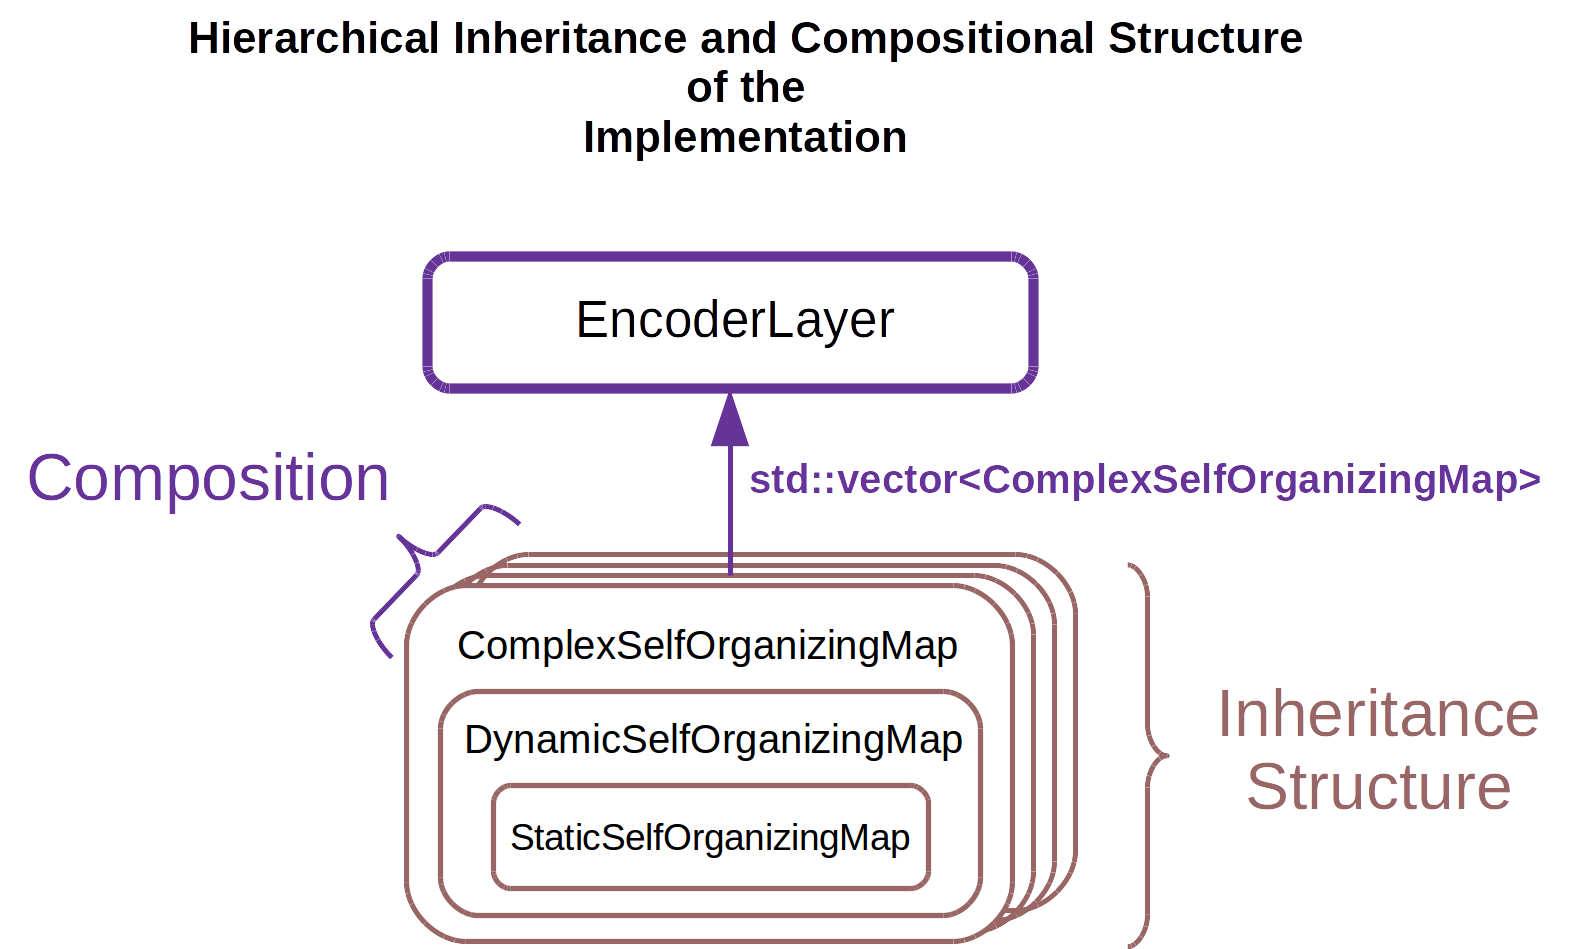
\includegraphics[width=0.8\textwidth]{Skeleton.png}
    %\caption{Hierarchical Inheritance and Compositional Structure of the Model Implementation.
    %\glsfirst{csom} inherits from \glsfirst{dsom} which inherits from \glsfirst{ssom}.
    %The \glsfirst{el} is formed by the composition of a set of \glspl{csom} gathered
    %in a std::vector \glsfirst{stl} container.}
    %\label{fig:Skeleton}
%\end{figure}

%\pagebreak

%We parallelize the \gls{el} class by means of a hybrid \gls{mpi}+\gls{omp} paradigm.
%We distribute \glspl{csom} among \gls{mpi} ranks as a deck of cards is distributed among different players.
%Each \gls{mpi} rank ends up with one or more \glspl{csom} and the \glspl{csom} in each rank are distributed
%among different \gls{omp} threads (Fig. \ref{fig:EncoderParallelization} A and B respectively).
%Information among \gls{mpi} ranks must be transferred in each time step.
%We gather all the information corresponding to the \glspl{csom}
%in each rank and then use \gls{mpi} Bcast function to transmit such information
%using a special comunication protocol by means of which we specify the boundaries
%in the information corresponding to each \gls{csom}(Fig. \ref{fig:EncoderParallelization} C).
%By means of this strategy each MPI rank has to call \gls{mpi} Bcast just once
%in order to transmit its data.
%The \gls{el} uses \gls{mpi} I/O parallel file system to save its status in Matlab/Octave format
%(Fig. \ref{fig:EncoderParallelization} D).
%Each \gls{mpi} rank gathers all the data corresponding to its \glspl{csom} in the \gls{el} and
%communicates the part of the file it will use to the other \gls{mpi} ranks, in order to store the data
%without interfering with the other ranks in the \gls{mpi} environment.
%Then, each \gls{mpi} rank saves all its data with a unique call to \gls{mpi} Write. 


%\begin{figure}[h!]
    %\centering
    %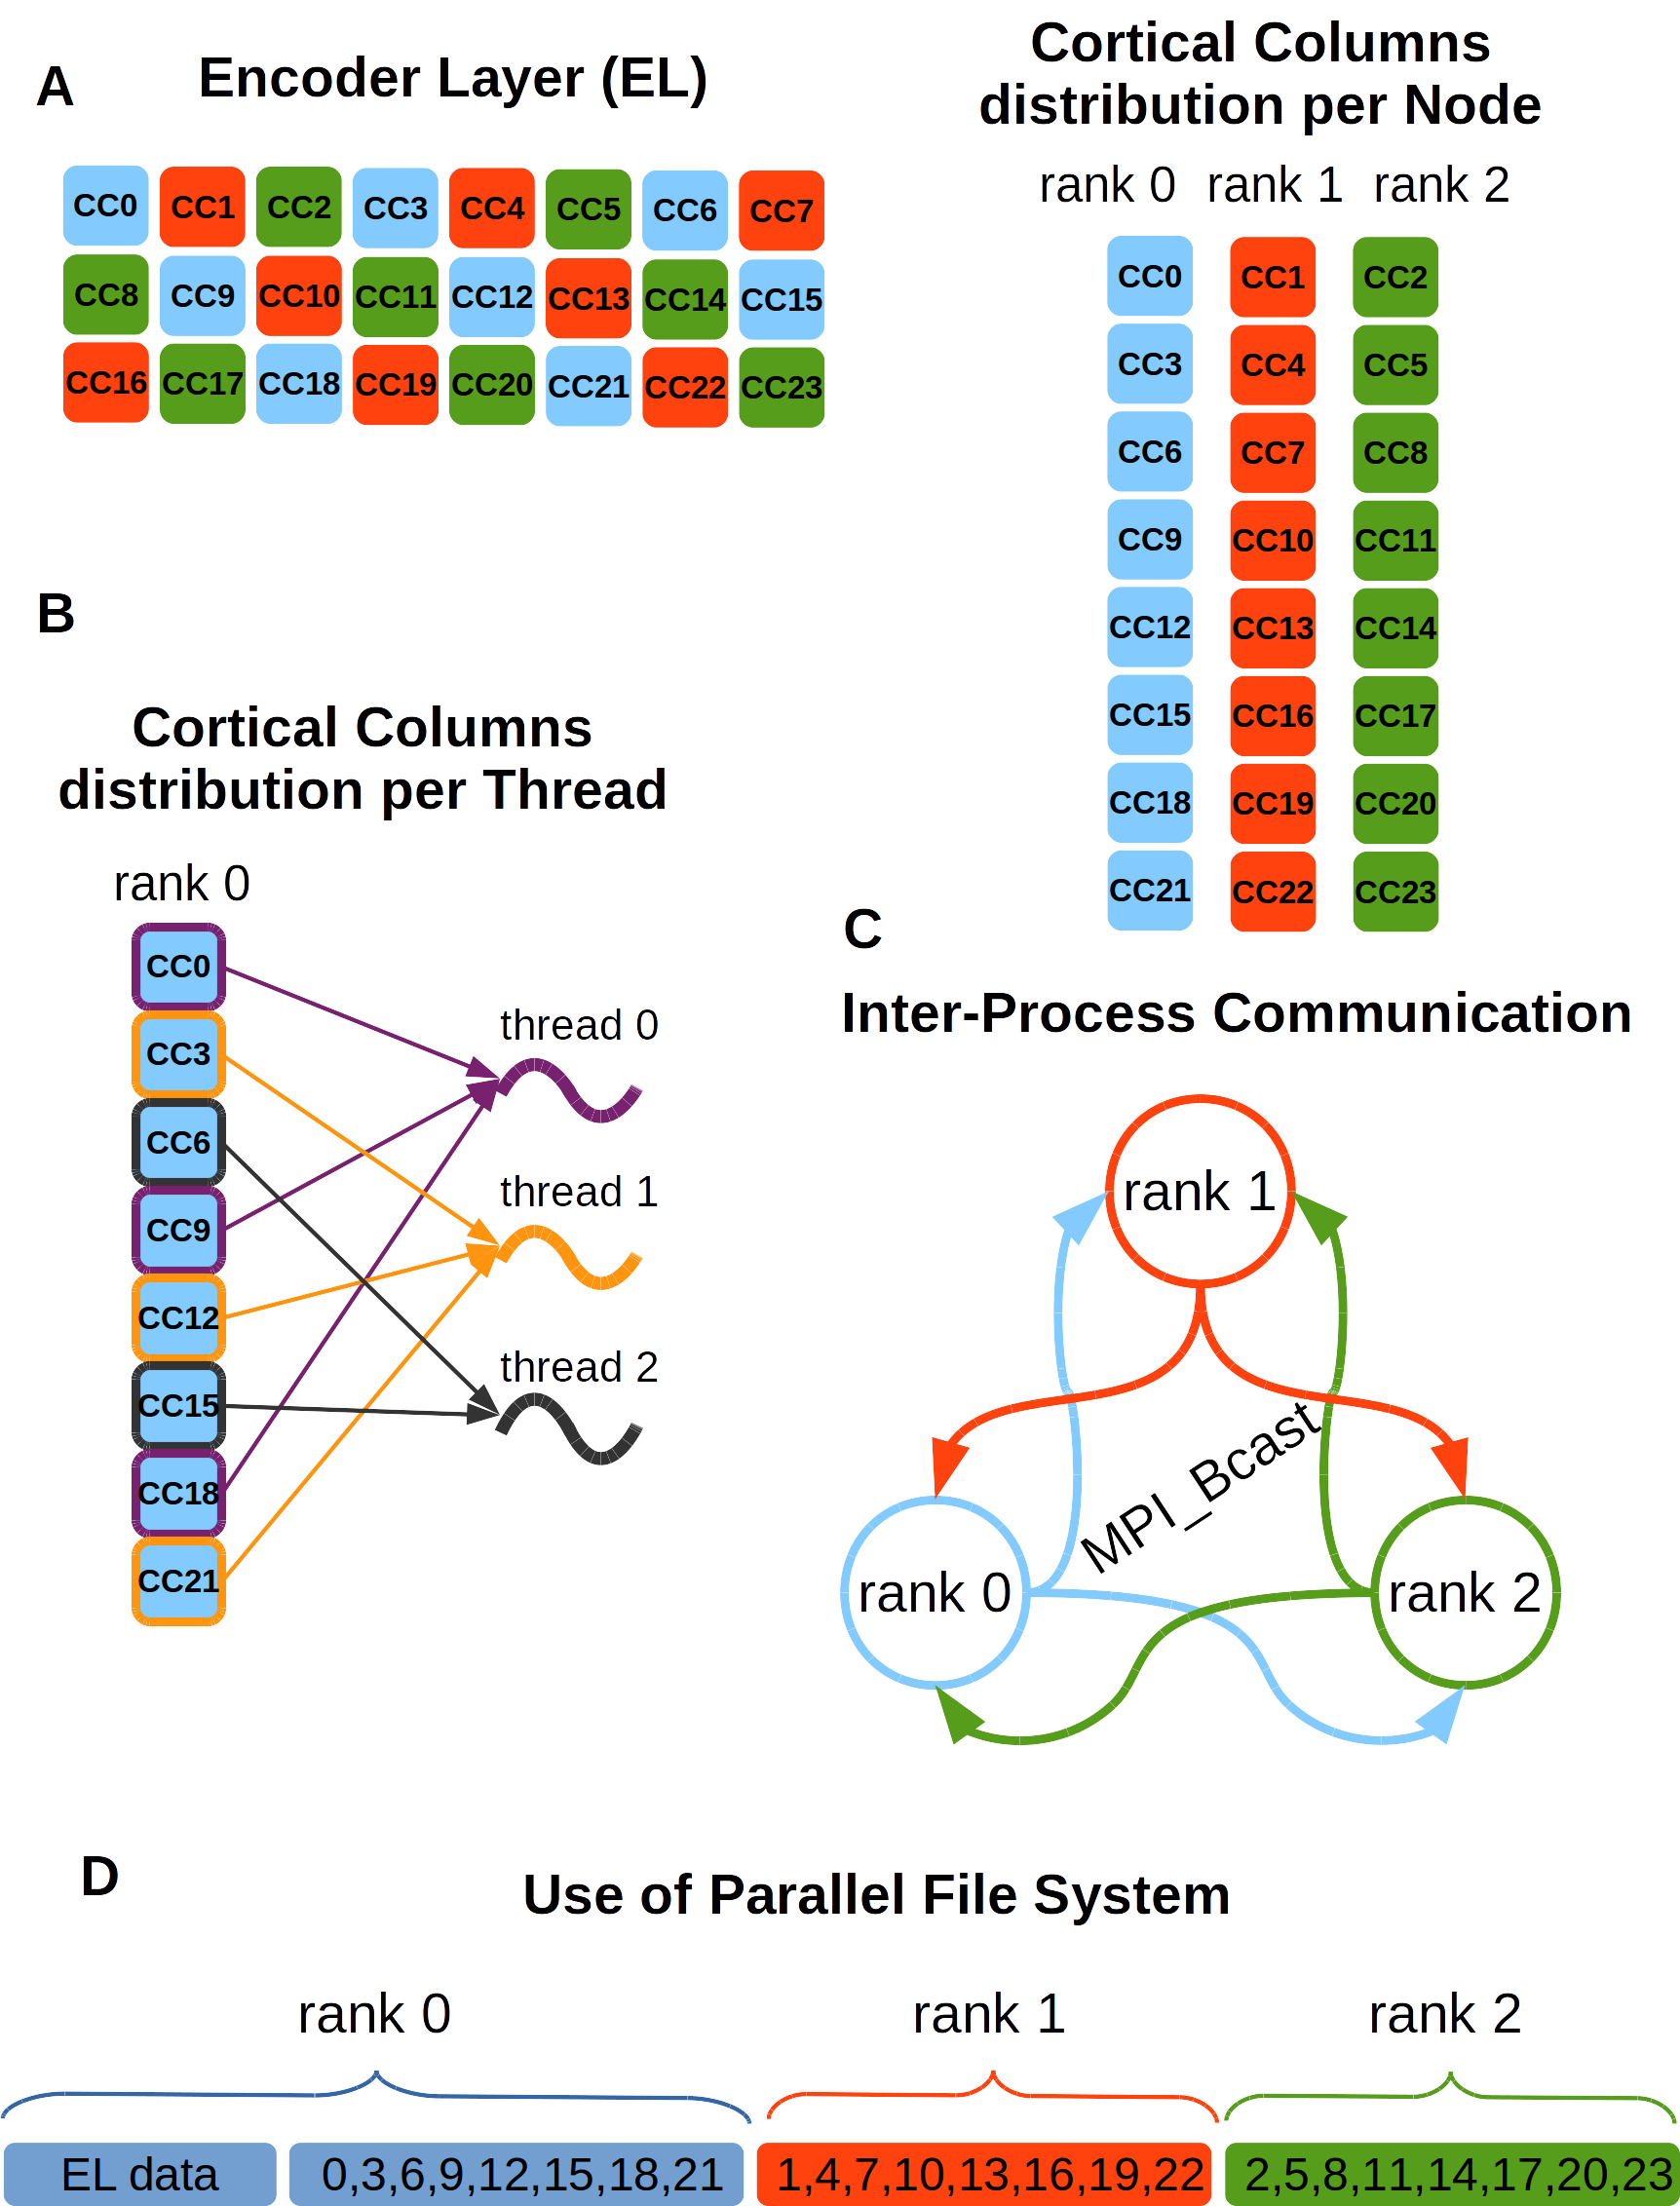
\includegraphics[width=0.75\textwidth]{EncoderParallelization.png}
    %\caption{\glsfirst{el} \gls{mpi}+\gls{omp} parallelization. (A) Distribution of \gls{csom} objects in an \gls{el} with
    %3 by 8 (24) \glspl{cc} among three \gls{mpi} ranks with three \gls{omp} threads per rank.
    %Certain ranks could take care of a different number of
    %\glspl{csom} depending on the number of \gls{mpi} ranks as well as the number of \glspl{cc} in the \gls{el}.
    %(B) Each \gls{mpi} rank distributes its \glspl{csom} among different threads in the same fashion.
    %(C) \gls{mpi} \gls{ipc} among different ranks. \gls{ipc} is carried out at each time step since each \gls{mpi} rank 
    %requires the complete \gls{el} output at each time step.
    %Each \gls{mpi} rank broadcasts the information corresponding to its \glspl{cc} to the other ranks in the \gls{mpi}
    %environment.
    %(D) \gls{el} information distribution in a file to save its status.
    %Each \gls{mpi} rank puts the formated data corresponding to its \glspl{csom} in a \gls{stl} stringstream class template.
    %Rank 0 also takes care of the \gls{el} structure, connectivity and parameters.
    %Once each rank has its stringstream with the formated data, it communicates its file view to the other ranks.
    %Then each rank writes its stream of bytes in parallel without interfering with other ranks in the \gls{mpi} environment.
    %An \gls{el} with a different number of ranks can load the same file without affecting the final results.
    %Each rank in the new \gls{el} loads the complete file in a \gls{stl} stringstream class template and then takes the
    %informations that concern it from such structure.}
    %\label{fig:EncoderParallelization}
%\end{figure}

%\pagebreak

%The implementation has Checkpoint and Restart capacity in its training stage where there is total flexibility
%in terms of the number of ranks with which the execution is restarted. A cortical layer could have been saved
%with $n$ ranks and such layer could be restarted with $m$ ranks without affecting the final results.


%It is important to mention that the number of \glspl{cc} shown in
%Fig. \ref{fig:EncoderParallelization} is merely illustrative and
%does not reflect the real numbers in terms of computational resources used for this implementation.

%%The simulations performed for this work were carried out in an \gls{alcf}
%%Allocation at \gls{anl}.
%%We run the algorithms on Cooley Cluster with simulations using 25 nodes 
%%(9 \glspl{cc} per node and one node per \gls{mpi} rank)
%%and 8 threads per node/rank (almost one thread per \gls{cc}).

%We performed all computational experiments on Cooley, a visualization and analysis cluster at Argonne National Laboratory. We ran the simulations using 25 nodes (9 \glspl{cc} per node and one node per \gls{mpi} rank) and 8 OpenMP threads per node/rank (almost one thread per \gls{cc}).



%~\\
%\noindent{\underline{\textit{Initial Strong and Weak Scaling Tests on Cooley}}}
%~\\
%~\\

%Beyond the fact that our computational approach is intended to be applied in leadership supercomputers in the future, in the present work an essential step is to test our code in order to see how it uses the resources provided by Cooley Nodes.
%Parallel scalability is a measurement that indicates how efficient is our code when using increasing numbers of parallel processing elements--Nodes or Processes and \glspl{cpu} or Threads on Cooley.
%Fig. \ref{fig:Strong_Weak} shows the scaling capacity of our code in terms of run time vs. number of processing elements used for the task.
%In our tests we always constrain our code to run one \gls{mpi} rank per Cooley node. Each \gls{mpi} rank spreads an specific number of threads through the different \glspl{cpu} in its corresponding node (Fig. \ref{fig:EncoderParallelization} A and B).
%There are two ways to measure the parallel performance of a given application. The measure to be applied will depend on whether the application is \gls{cpu}-bound or memory-bound. Such measurements are referred to as \emph{strong} and \emph{weak} scaling, respectively.



%\begin{figure}[h!]
    %\centering
    %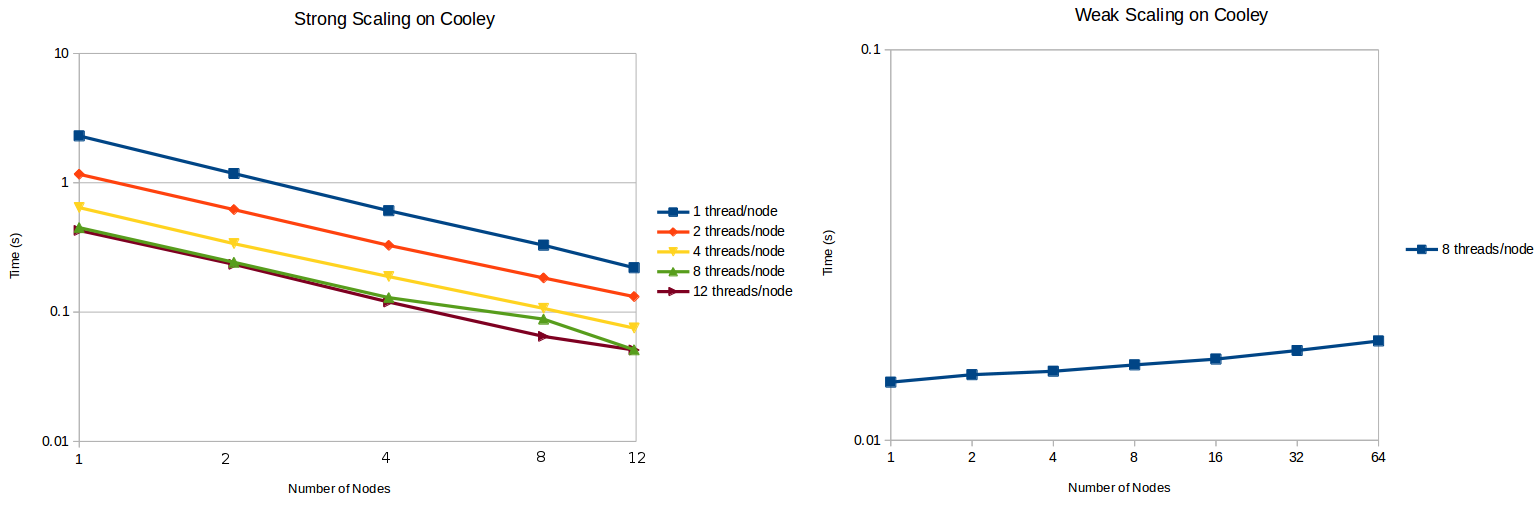
\includegraphics[width=1.0\textwidth]{Strong_Weak.png}
    %\caption{Strong and Weak scaling tests on Cooley nodes. Left: Strong scaling. Run time vs. the number of nodes for different number of threads per node.
	    %The problem size stays fixed but the number of processing elements are increased.
    %Right: Weak scaling. Run time vs. the number of nodes for different number of threads per node.
    %In this case the problem workload assigned to each processing element stays constant and additional elements are used to solve a larger total problem (i.e. a problem that would not fit in the available RAM on a single node).}
    %\label{fig:Strong_Weak}
%\end{figure}

%\pagebreak


%%~\\
%%\noindent{\textit{Strong Scaling}}
%%~\\
%%~\\

%%In strong scaling, it is considered that a program scales linearly when the time spent by the run is reduced in proportion to the number of processing elements used ($N$).
%%If the amount of time to complete a run with 1 processing element is $t_1$, and the amount of time spent to complete the same run with $N$ processing elements is $t_N$, the strong scaling efficiency is~\cite{scaling}:

%%\begin{equation}
	%%t_1/(N * t_N) * 100
%%\end{equation}

%%In the present work we achieved an efficiency in strong scaling of 70\% with 12 Nodes and 12 threads per node.

%%~\\
%%\noindent{\textit{Weak Scaling}}
%%~\\
%%~\\

%%In the case of weak scaling, linear scaling is achieved if the run time stays constant while the workload is increased in direct proportion to the number of processors.
%%If the amount of time to complete a run with 1 processing element is $t_1$, and the amount of time to complete $N$ of the same runs with $N$ processing elements is $t_N$, the weak scaling efficiency (as a percentage of linear) is given as~\cite{scaling}:

%%\begin{equation}
	%%t_1/t_N * 100
%%\end{equation}

%%In the present work we achieved an efficiency in weak scaling of 78.4\% with 64 Nodes and 8 threads per node.

%%Fig.~\ref{fig:Strong_Weak_Efficiency} shows strong and weak scaling efficiencies for different number of processing elements--nodes in the present work.
%%\begin{figure}[h!]
    %%\centering
    %%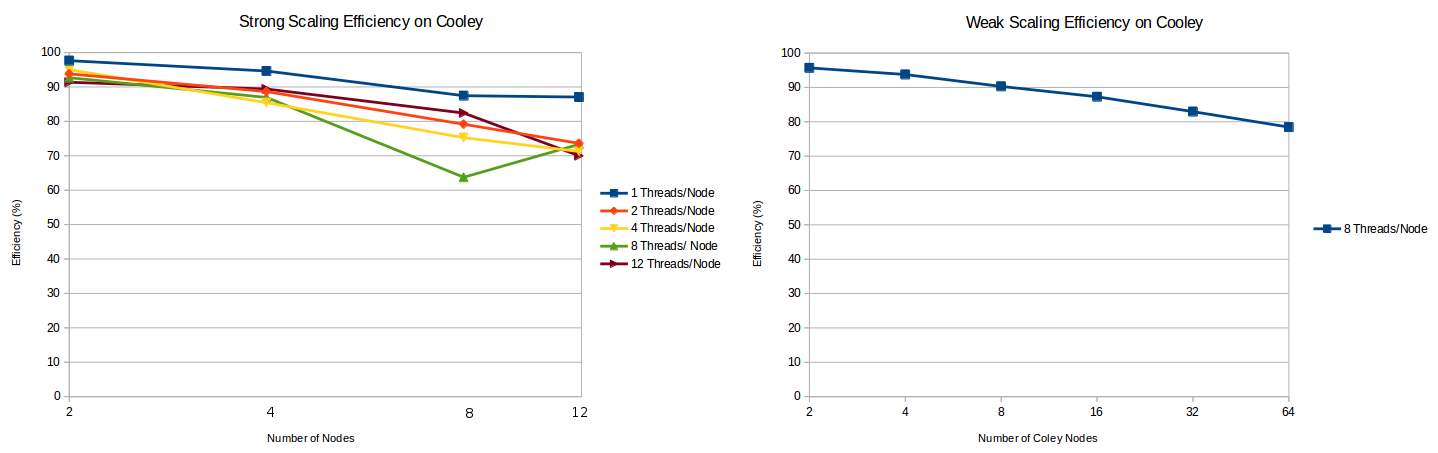
\includegraphics[width=1.0\textwidth]{Strong_Weak_Efficiency.png}
    %%\caption{Strong and Weak scaling efficiency measures on Cooley nodes. Left: Strong scaling efficiency measures. Efficiency vs. the number of nodes for different number of threads per node.
    %%Right: Weak scaling efficiency measures. Efficiency vs. the number of nodes for 8 threads per node.}
    %%\label{fig:Strong_Weak_Efficiency}
%%\end{figure}

%%\pagebreak

%%As can be seen in Fig. \ref{fig:Strong_Weak_Efficiency} we have an efficiency in the use of the resources that is well above 60\% for strong scaling tests and well above 70\% for weak scaling tests on Cooley nodes. These results are supported by the linearity exhibited in Fig. \ref{fig:Strong_Weak} (left) and by the small slope in the line shown in Fig. \ref{fig:Strong_Weak} (right).



%Straight lines in Fig. \ref{fig:Strong_Weak} (left) show an initially good strong scalability of our code while the small slope exhibited by Fig. \ref{fig:Strong_Weak} (right) allows us to foresee a good weak scaling performance of our code in high end leadership supercomputers.











\subsubsection*{Experiments}

In the present work, we studied the level of invariance in the phonetic features abstracted by the \gls{el}, by means of comparing such representations with the multiresolution spectro-temporal auditory features returned by the \gls{mrstsa} algorithm. To this end, we evaluated the features returned by each algorithm in different word classification tasks. \reviewertwo{In order to asses word classification performance} in each algorithm, \reviewertwo{we used the \gls{svm} technique}--section \nameref{model-implementation}--with  the experimental setup depicted in Fig. \ref{fig:Experiment}.

\begin{figure}[h!]
    \centering
    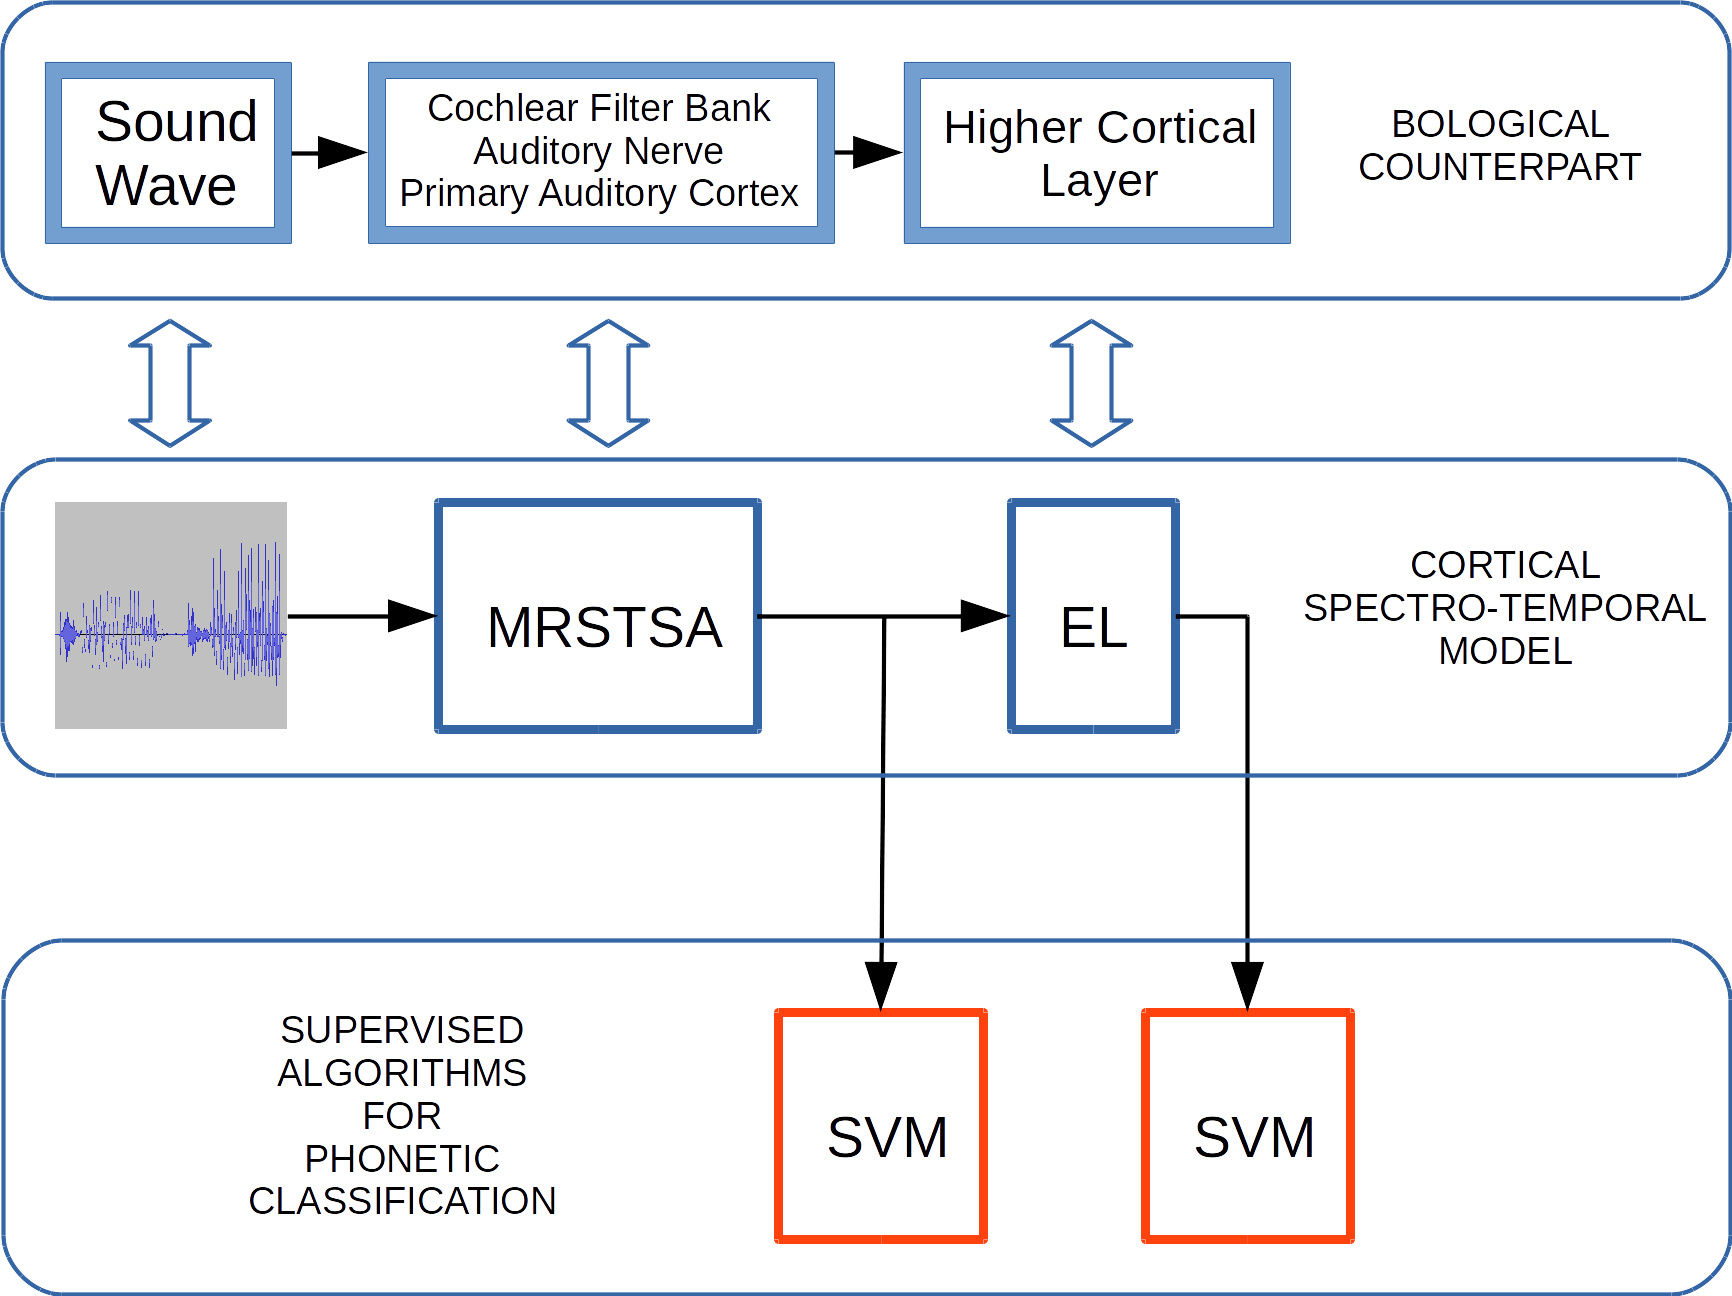
\includegraphics[width=0.8\textwidth]{Experiment.png}
    \caption{Experimental setup to test word classification task performances.
    Sound waves are processed by the \gls{mrstsa} algorithm.
    The outputs from the \gls{mrstsa} are processed by the \gls{el}.
    Word classification tasks are performed on both outputs by the \gls{svm} algorithm.
    Each section in the \gls{cstm} has its biological counterpart.}
    \label{fig:Experiment}
\end{figure}

\pagebreak

\reviewerfour{In the experimental procedure we first trained 10 different \glspl{el}--section \nameref{model-implementation}--for each syllabic condition. Such \glspl{el} were trained using the voices in set one and the corpora were generated by the method described in section \nameref{CorpGen}. Afterwards, we processed the same corpora with the corresponding \glspl{el} in inference mode. In such mode, the \glspl{el} processed the information with their learning properties disabled. In this manner, during inference, the \glspl{el} did not modify its synapses and just returned patterns of activation in response to the stimuli they received. We then used the outputs from the \gls{mrstsa} and the \glspl{el} in inference mode to train the \gls{svm} classifiers with the procedure depicted in section \nameref{model-implementation}. The average cross validation training performances are shown in Table~\ref{SVM_Training}}.

\begin{table}[h!]
\centering
\caption{\gls{svm} 5-fold cross validation training results}
\begin{tabular}{|l|l|l|}
\hline
                   & MRSTSA & Encoder Layer \\ \hline
Monosyllabic Words & 99.4\% & 99.52\%          \\ \hline
Disyllabic Words   & 99.3\%   & 99.48\%        \\ \hline
Trisyllabic Words  & 99.5\% & 99.58\%          \\ \hline
\end{tabular}
\label{SVM_Training}
\end{table}

\pagebreak

\reviewerfour{In a second stage, we ran the \glspl{el} in inference mode again, but \reviewertwo{this time we used different corpora generated using the same voices and manipulated with several types of acoustic variants (white noise, reverberation and pitch variations), generated using the Audacity software}. We also ran the \glspl{el} in inference mode using corpora generated with different voices (set two voices in section \nameref{CorpGen}). We tested the performances of the--already trained--classifiers in the presence of the features returned by the algorithms in response to the corpora affected by the \reviewertwo{acoustic variants} which we introduced to the new corpora by means of Audacity \cite{audacity}. The \reviewertwo{acoustic variants} introduced to the new corpora included white noise, reverberation and pitch variations. We also tested the classifier performances in the presence of the features returned by the algorithms in response to the new corpora generated with a different set of voices}.











\section*{Results}

The classification performances are shown in Fig. \ref{fig:PLOT}.

\begin{figure}[h!]
    \centering
    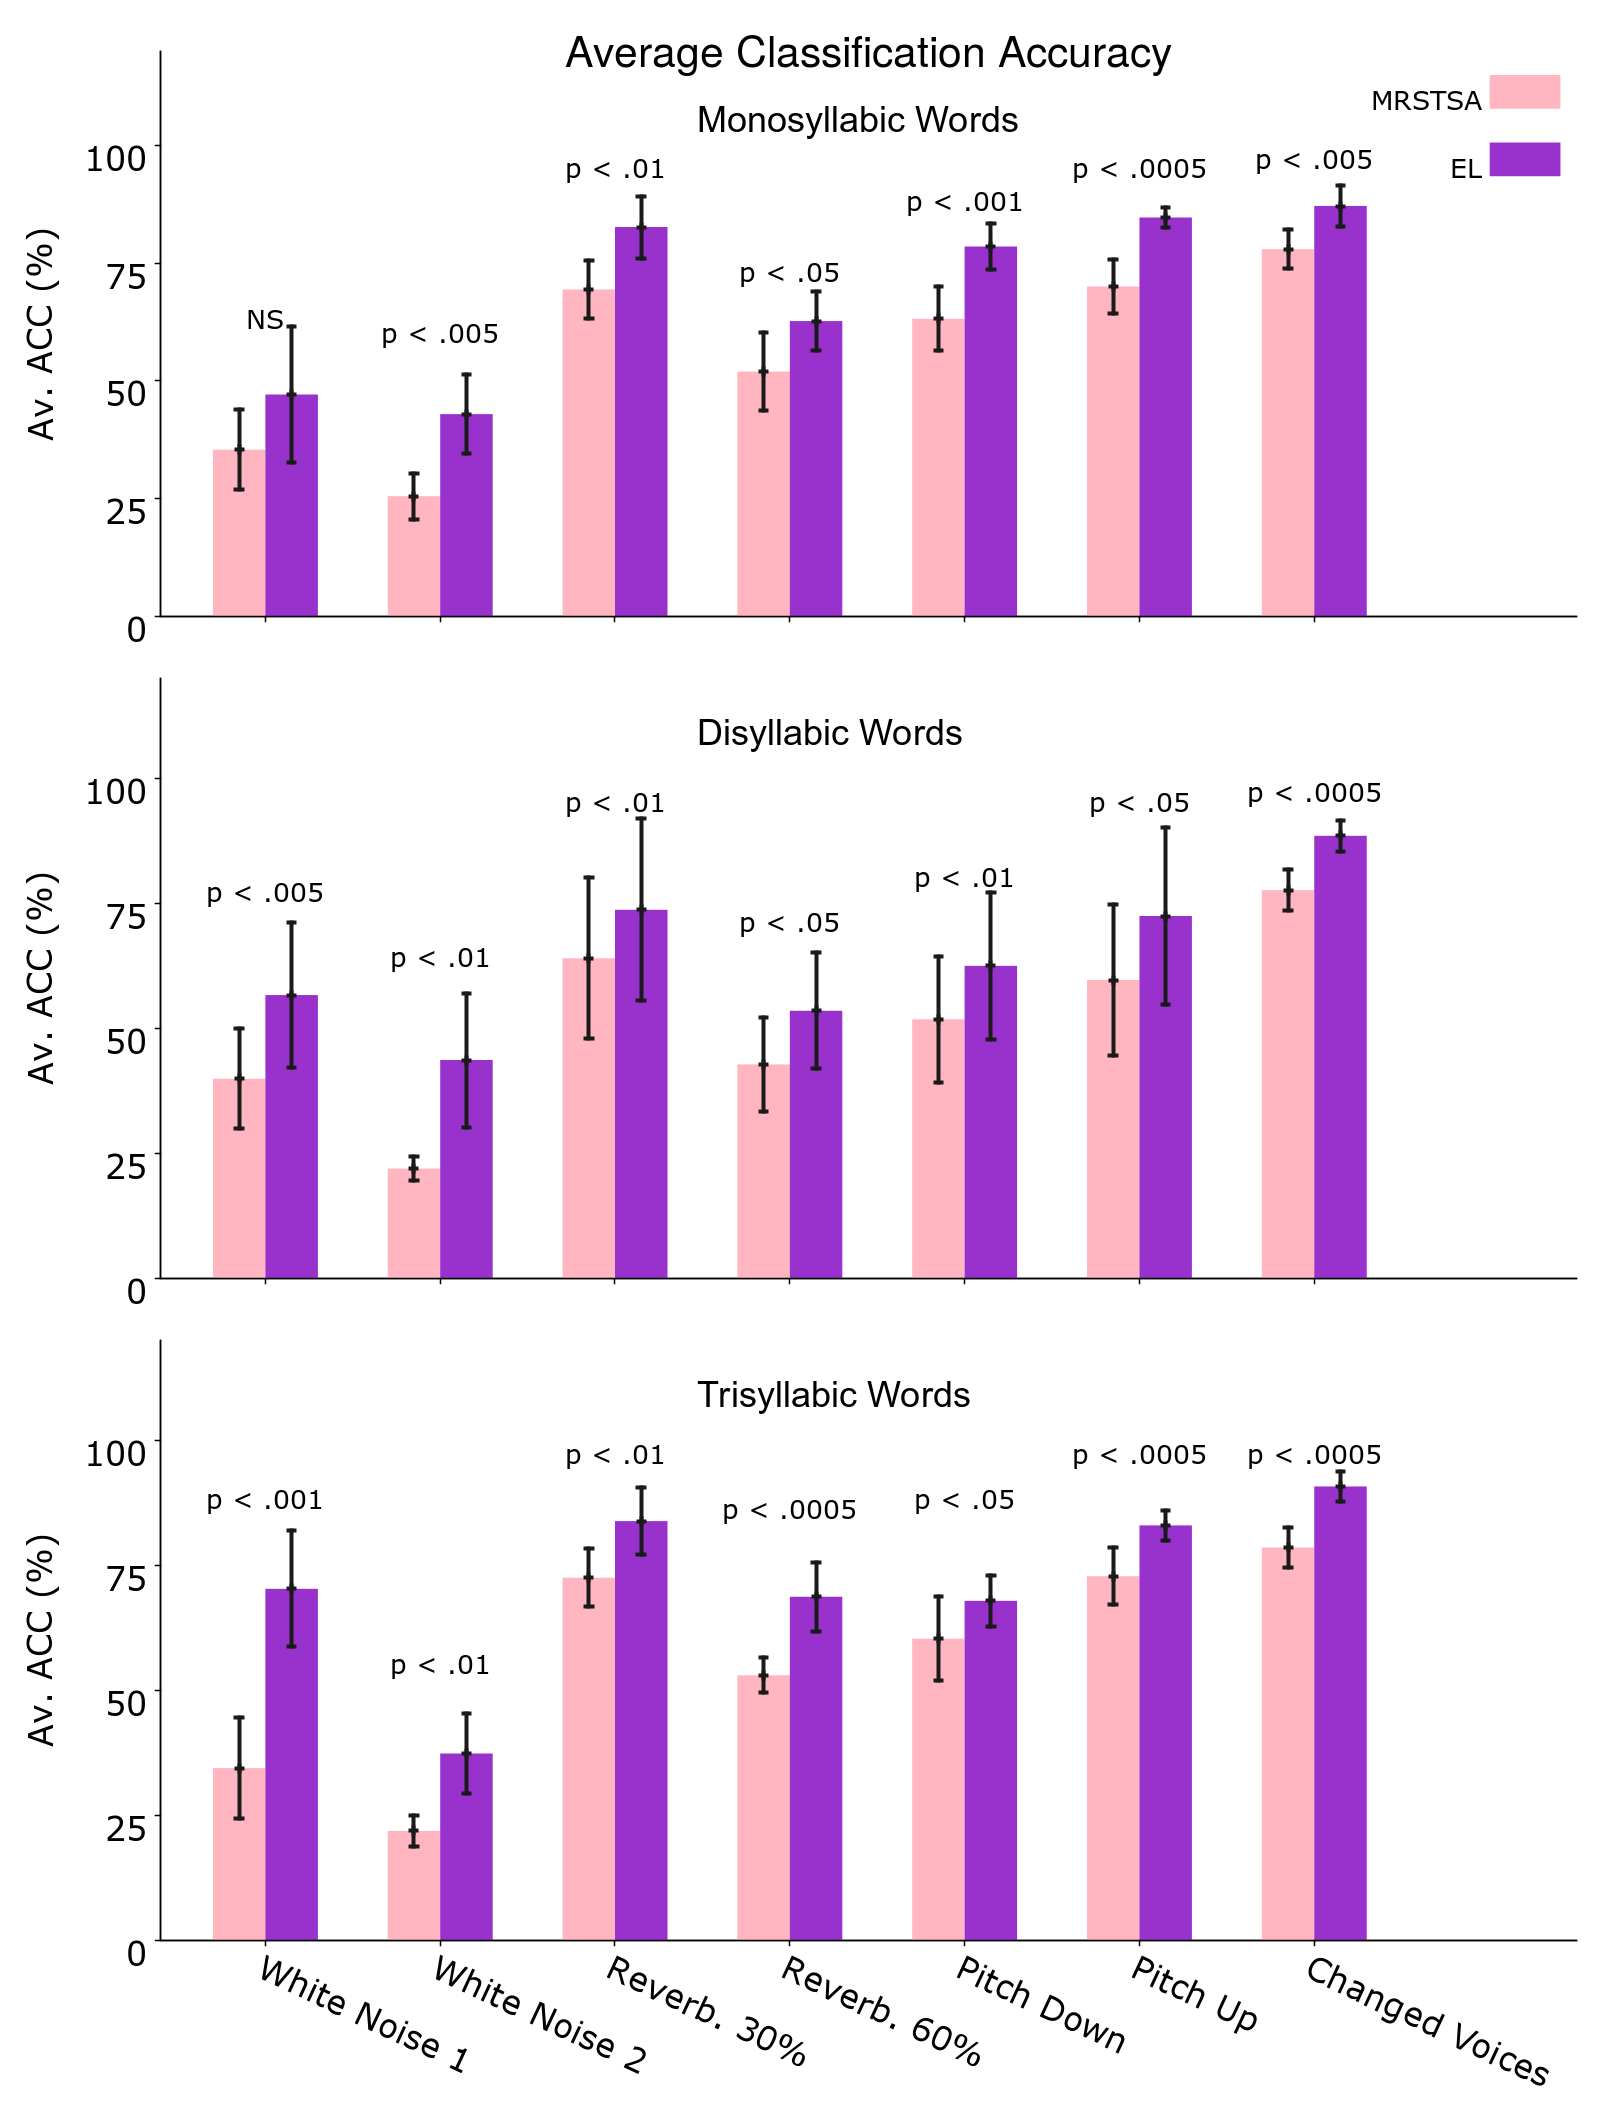
\includegraphics[width=0.9\textwidth]{PLOT.png}
    \caption{\gls{mrstsa} and \gls{el} average classification accuracies against different \reviewertwo{acoustic variants} introduced to the signals
    for monosyllabic, disyllabic and trisyllabic words.
    White Noise 1 determines a \gls{snr} average \gls{rms} power rate of 19.8 dB while White Noise 2 13.8 dB.
    Reverberation 30\% determines a \gls{rt} value of 0.61 seconds while Reverberation 60\% determines a \gls{rt} value of 1.78 seconds.
    Pitch Up determines a pitch move from E to G, while Pitch Down determines a pitch move from E to C. Changed Voices corresponds to corpora generated using a different set of voices from the one used to train the \glspl{el} and the classifiers. \reviewertwo{Error bars depict 95\% Confidence Interval values. The \emph{p} values correspond to one-tailed paired t-tests and NS stands for Not Statistically Significant.}}
    \label{fig:PLOT}
\end{figure}

%\begin{figure}[h!]
    %\centering
    %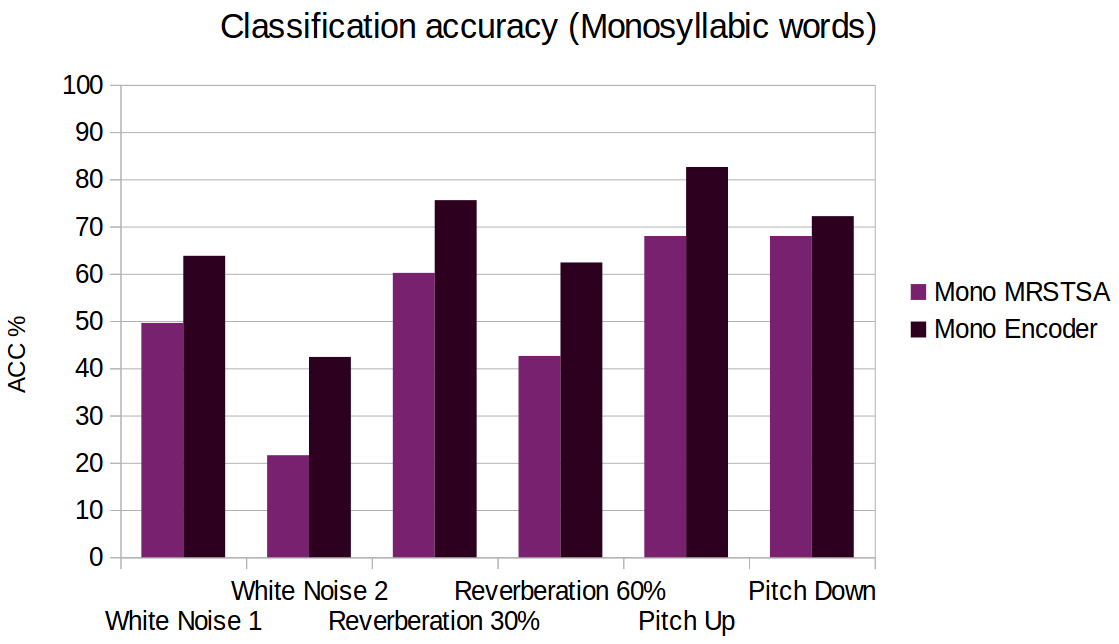
\includegraphics[width=0.9\textwidth]{MONO_ACC.png}
    %\caption{\gls{mrstsa} and \gls{el} classification accuracies against different \reviewertwo{acoustic variants} introduced to the original signals
    %for \textbf{monosyllabic words}.
    %White Noise 1 determines a \gls{snr} average \gls{rms} power rate of 19.8 dB while White Noise 2 13.8 dB.
    %Reverberation 30\% determines a \gls{rt} value of 0.61 seconds while Reverberation 60\% determines a \gls{rt} value of 1.78 seconds.
    %Pitch Up determines a pitch move from E to G, while Pitch Down determines a pitch move from E to C.}
    %\label{fig:MONO_ACC}
%\end{figure}

%\begin{figure}[h!]
    %\centering
    %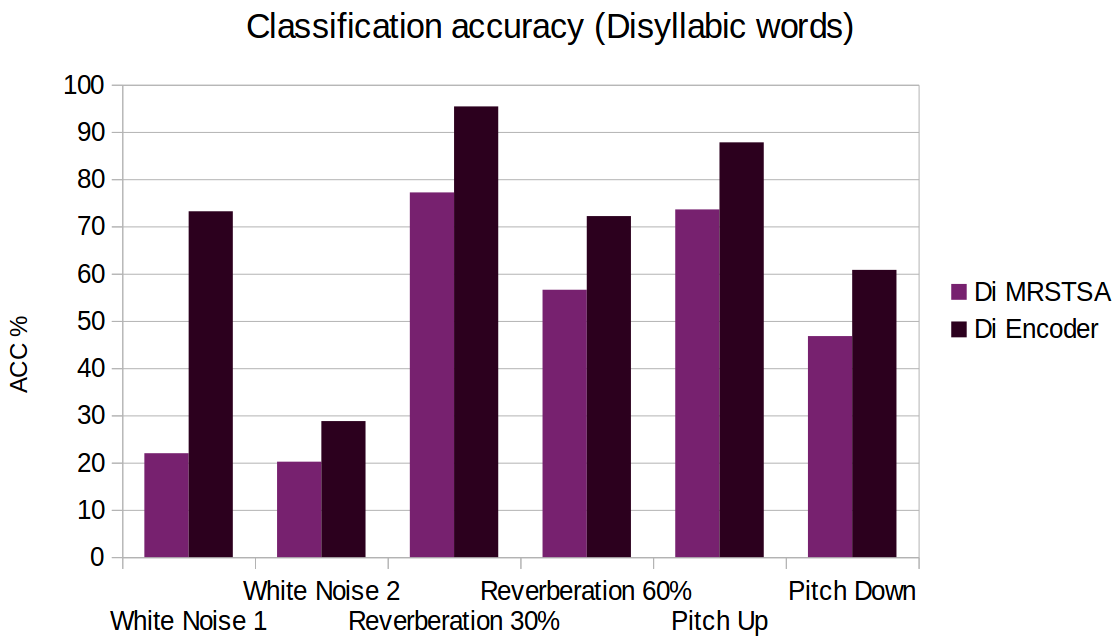
\includegraphics[width=0.9\textwidth]{DI_ACC.png}
    %\caption{\gls{mrstsa} and \gls{el} classification accuracies against different \reviewertwo{acoustic variants} introduced to the original signals
    %for \textbf{disyllabic words}.
    %White Noise 1 determines a \gls{snr} average \gls{rms} power rate of 19.8 dB while White Noise 2 13.8 dB.
    %Reverberation 30\% determines a \gls{rt} value of 0.61 seconds while Reverberation 60\% determines a \gls{rt} value of 1.78 seconds.
    %Pitch Up determines a pitch move from E to G, while Pitch Down determines a pitch move from E to C.}
    %\label{fig:DI_ACC}
%\end{figure}

%\begin{figure}[h!]
    %\centering
    %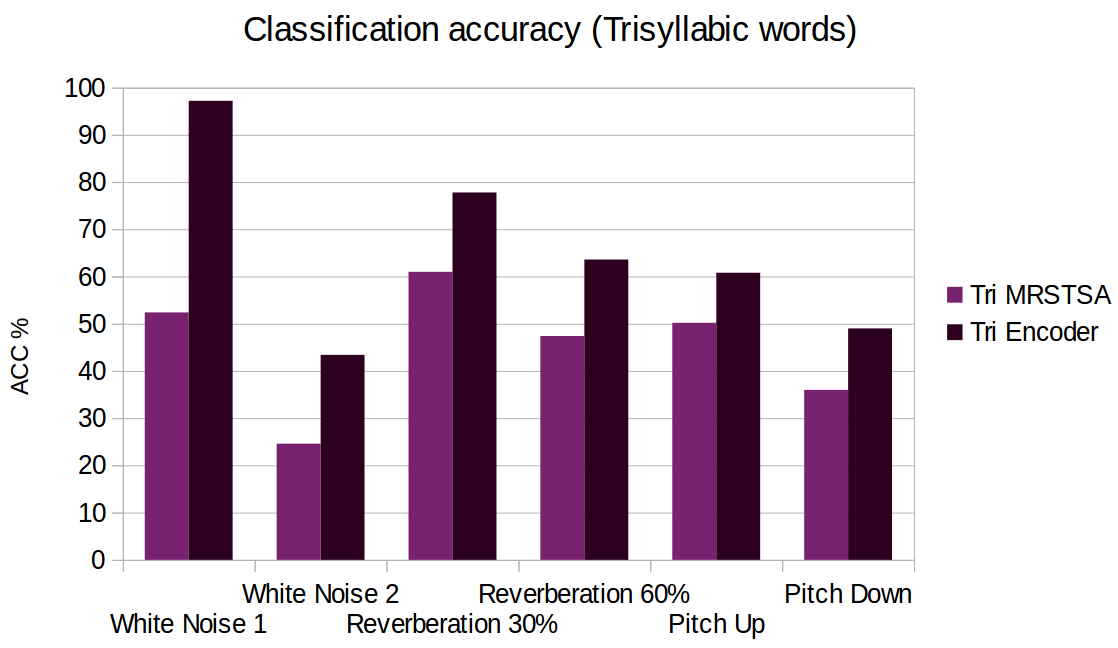
\includegraphics[width=0.9\textwidth]{TRI_ACC.png}
    %\caption{\gls{mrstsa} and \gls{el} classification accuracies against different \reviewertwo{acoustic variants} introduced to the original signals
    %for \textbf{trisyllabic words}.
    %White Noise 1 determines a \gls{snr} average \gls{rms} power rate of 19.8 dB while White Noise 2 13.8 dB.
    %Reverberation 30\% determines a \gls{rt} value of 0.61 seconds while Reverberation 60\% determines a \gls{rt} value of 1.78 seconds.
    %Pitch Up determines a pitch move from E to G, while Pitch Down determines a pitch move from E to C.}
    %\label{fig:TRI_ACC}
%\end{figure}

%\pagebreak

Regarding white noise, we introduced additive white noise to the corpora signals with signal-noise average \gls{rms} power rate of 19.9 dB (White Noise 1) and 13.8 dB (White Noise 2). In terms of reverberation, we modified the corpora signals by means of \gls{rt} values of 0.61 seconds (Reverberation 30\%) and 1.78 seconds (Reverberation 60\%). \gls{rt} Is the time that a signal takes to decrease its amplitude to 60 dBs under its initial value. As regards pitch variations, we modified the corpora signals pitch in +20\% (from E to G) (Pitch Up) and in--20\% (from E to C) (Pitch Down). \reviewerfour{We also used corpora generated with different voices from the ones used to train the \glspl{el} and the \glspl{svm}}.

\iffalse
\begin{figure}[h!]
    \centering
    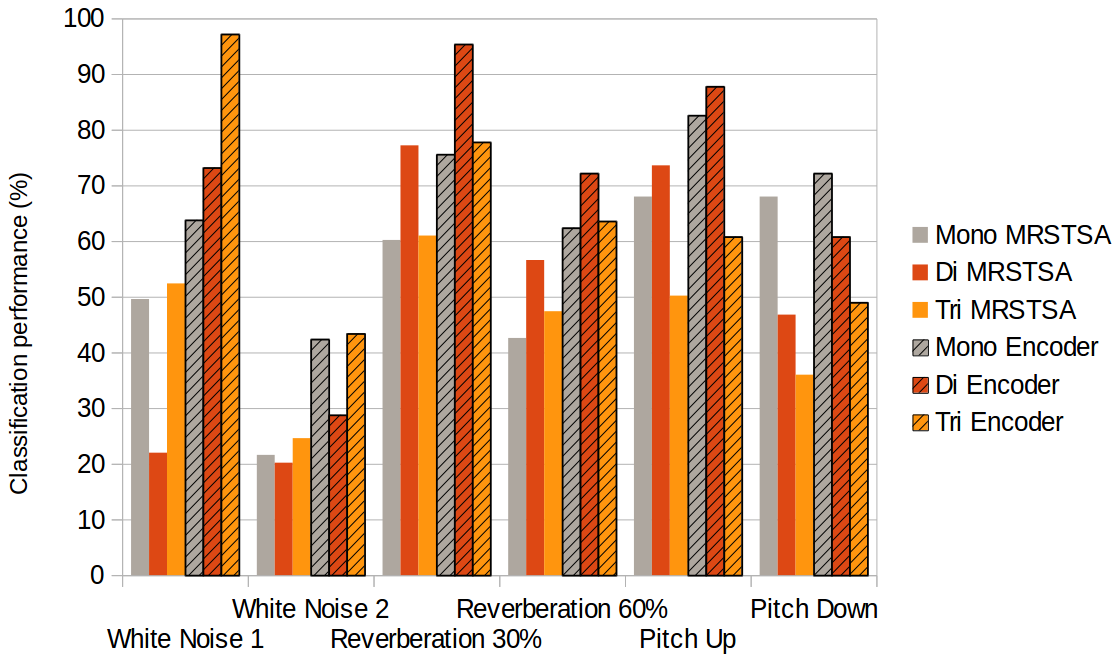
\includegraphics[width=0.9\textwidth]{Classification.png}
    \caption{\gls{mrstsa} and \gls{el} classification performances against different \reviewertwo{acoustic variants} introduced to the original signals.
    Mono means monosyllabic words, Di means disyllabic words and Tri means trisyllabic words.
    White Noise 1 determines a \gls{snr} average \gls{rms} power rate of 19.8 dB while White Noise 2 13.8 dB.
    Reverberation 30\% determines a \gls{rt} value of 0.61 seconds while Reverberation 60\% determines a \gls{rt} values of 1.78 seconds.
    Pitch Up determines a pitch move from E to G, while Pitch Down determines a pitch move from E to C.}
    \label{fig:Classification}
\end{figure}
\fi


Fig. \ref{fig:PLOT}
\reviewertwo{shows a 5-way word classification accuracy} for mono, di and trisyllabic word corpora affected by
white noise, reverberation and pitch \reviewerfour{and voice} variations.
As can be seen in the figures, the \gls{el} outperforms the \gls{mrstsa} in all cases.
Such behavior persists for multisyllabic words.

\reviewertwo{We performed one-tailed paired t-tests for 10 different corpora generated from 10 different vocabularies--section \nameref{CorpGen}. As can be seen in Fig. \ref{fig:PLOT}--except for monosyllabic words with White Noise 1 $(p < 0.11)$--there was Statistical Significance for all conditions considering $(p<0.05)$}.

Fig. \ref{fig:AV_ACC} shows average classification accuracies across all \reviewertwo{acoustic variants} for mono, di and trisyllabic words.
\reviewertwo{In this case, we also performed one-tailed paired t-tests, but this time for 7 different acoustic variant conditions.
As can be seen in the figure, all performed tests are statistically significant and the encoder layer clearly shows
a sustained superiority across words with different number of syllables}.
 

\begin{figure}[h!]
    \centering
    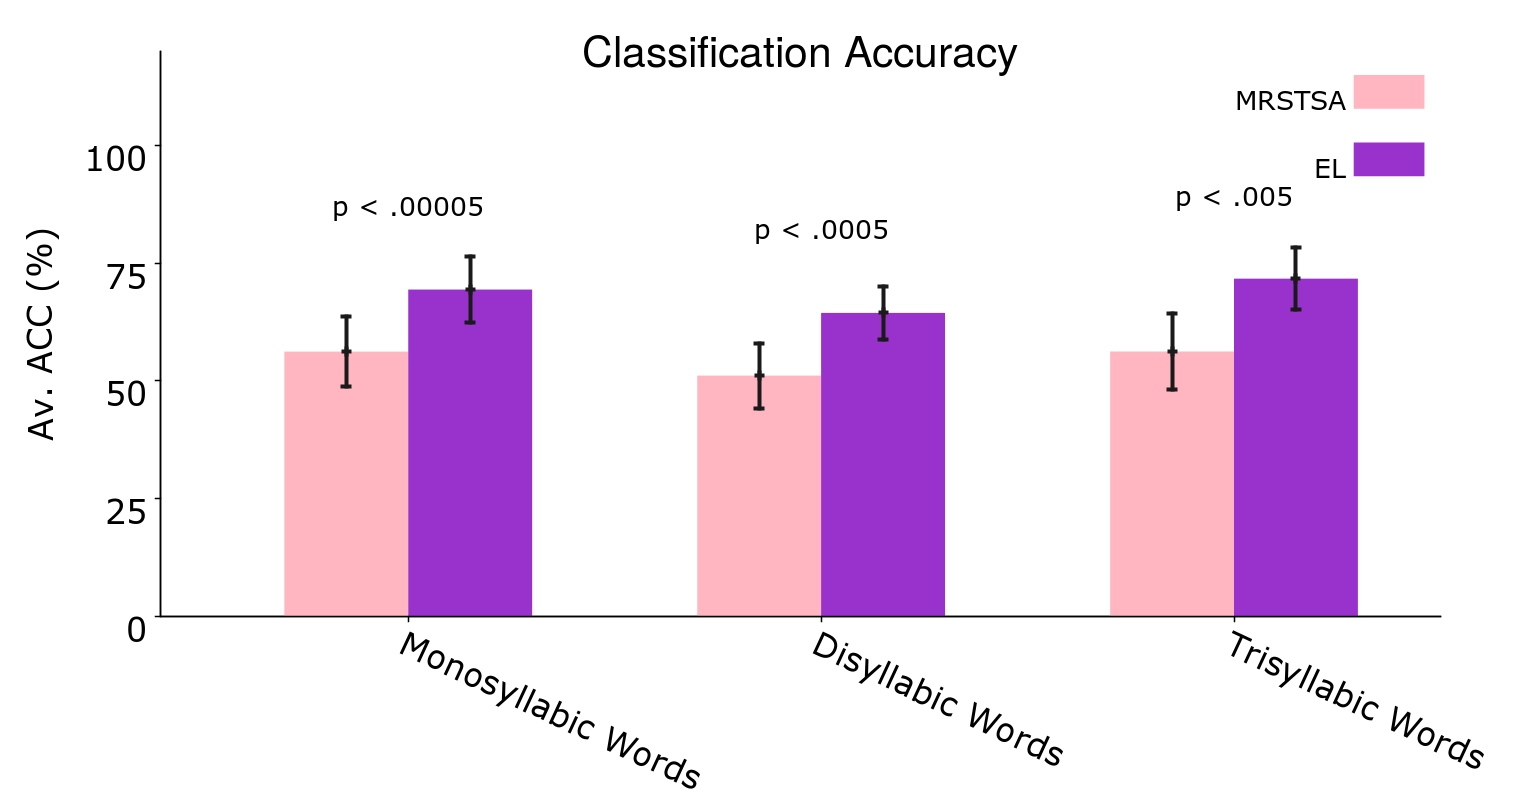
\includegraphics[width=0.9\textwidth]{PLOT1.png}
    \caption{Average classification accuracies across all \reviewertwo{acoustic variants} for mono, di and trisyllabic words. \reviewertwo{Error bars depict 95\% Confidence Interval values. The \emph{p} values correspond to one-tailed paired t-tests}.}
    \label{fig:AV_ACC}
\end{figure}

%\begin{figure}[h!]
    %\centering
    %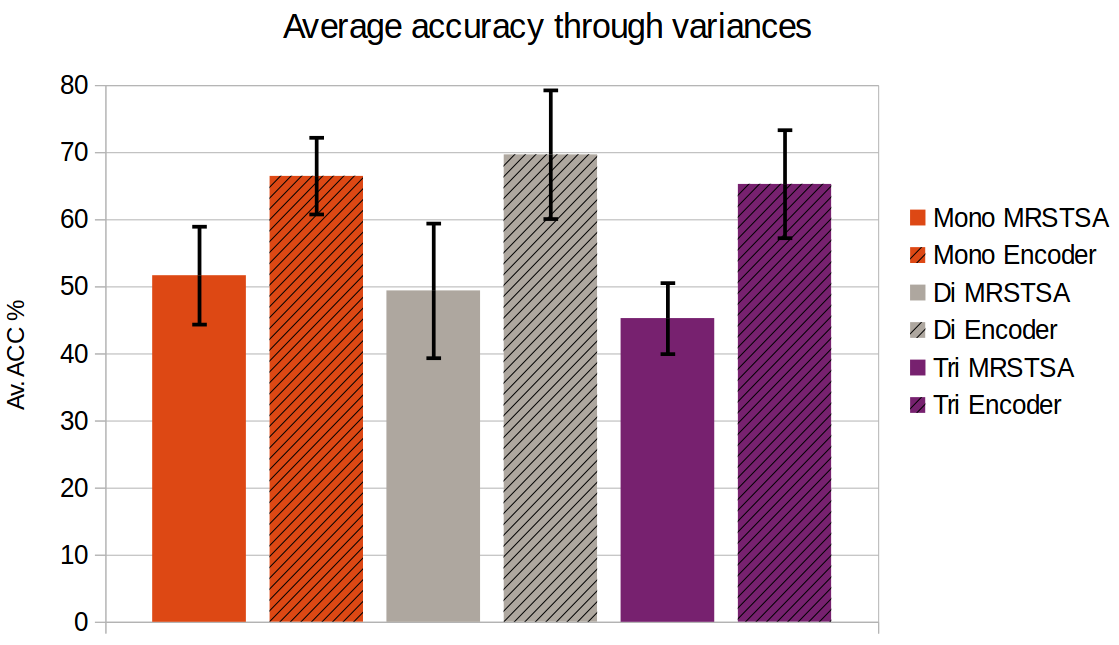
\includegraphics[width=0.9\textwidth]{AV_ACC.png}
    %\caption{Average classification accuracies across all \reviewertwo{acoustic variants} for mono, di and trisyllabic words with Standard Error bars.
    %Mono means monosyllabic words, Di means disyllabic words and Tri means trisyllabic words.}
    %\label{fig:AV_ACC}
%\end{figure}













\section*{Discussion}

%Results obtained in the present work support the hypothesis that certain neuroanatomical and neurophysiological features--mainly in cortical tissue--might be crucial for auditory perceptual phonetic invariance.
%These features have already been explained in terms of their properties \cite{hawkins_2016}, but more specifically in terms of their sequence learning capabilities \cite{cui_2016}.
\reviewerfour{Results obtained in the present work support the computational hypotheses posed in our modeling approach in order to mimic incidental phonetic invariance and generalization.
Some of these hypotheses have already been explained in terms of their properties \cite{hawkins_2016}, but more specifically in terms of their sequence learning capabilities \cite{cui_2016}}.
Nevertheless, there are no precedents of such neurophysiological features tested in word classification tasks as the ones carried out here, in which phonotactic rules are acquired \reviewerfour{without the application of optimization procedures such as backpropagating errors by means of gradient descent}. In addition, our approach presents substantial differences in terms of feature algorithmic implementation. In the present work, distal synapses make continuous individual contributions and our anatomical micro-columnar organization acquires its physiological behavior spontaneously from learning. We also tested such features in a realization with hundreds of cortical columns each combining several micro-columns with stochastic afferent activation whose future implementations are intended to explode large-scale simulations in leadership supercomputers.% (see section \nameref{Comp_setup}).

Computational models have been previously developed to understand how phonetic categories are acquired~\cite{rasanen_2012}. The goal in these works has been mainly to explain relevant aspects of phonetic acquisition, without details about how the brain might provide such computations. 
Lee et al. (2009), employed unsupervised feature learning for audio classification with \glspl{cdbn}~\cite{Lee:2009:UFL:2984093.2984217}.
The authors tested classification performance of a model with two layers in a 39-way phone classification accuracy task on the test data \gls{timit} for various numbers of training sentences.
The first layer never outperformed the \gls{mfcc} algorithm that was used as input for the network.
Furthermore, such work did not report the second layer performance since it could not outperform the first one.
The maximum performance reported for the first layer was 64.4\% vs. a performance of 79.6\% for the \gls{mfcc}.
It was just possible to report a performance of 80.3\% by means of combining both, the \gls{mfcc} and the first layer in the \gls{cdbn}.

In a more recent work, the capacity of \glspl{dmn}--a modification of \glspl{dnn} feed-forward architecture that uses a max-out activation function--to handle environmental noise was investigated into different broad phonetic classes and for different noise conditions \cite{silos_2016}.  In such experiments--with the exception of fricatives phonemes for 15 dB \gls{snr} Street Noise--accuracy never exceeded 70\%. Furthermore, performance was seriously impaired in the presence of 15 dB \gls{snr} white noise, resulting in classification accuracy  well below 60\% in all cases.

% TODO This will probably have to be modified to support new experiments
\reviewerfour{In the present work, we reported classification performances of--for example--90.8\% on the \gls{el} vs. 78.58\% on the \gls{mrstsa} for trisyllabic words against Changed Voices (i.e. voices never ``heard'' by the \gls{el} during training; Fig. \ref{fig:PLOT}), we also reported a performance above 70\% on the \gls{el} vs. a performance below 35\% on the \gls{mrstsa} for trisyllabic words against 19.8 dB \gls{snr} white noise and performances well above 40\% for mono and disyllabic words against 13.8 dB \gls{snr} white noise (Fig. \ref{fig:PLOT}). We also reported that the \gls{el} outperformed the \gls{mrstsa} for all the test conditions and that this behavior was sustained through different number of syllables in the words by means of statistical significance tests (Fig. \ref{fig:AV_ACC})}.

Although this is a compelling scenario, we have to be cautious since we cannot ignore important experimental differences from previous research results. First, our training material was very different from that found in previous works. We used corpora generated by synthesized voices instead of standardized \gls{timit} corpora.
\reviewerfour{Our main aim was to mimic early phonetic acquisition in humans, which is incidentally accomplished by infants \cite{Saffran1996StatisticalLB}}.
Given the high quality of the voices synthesized by \gls{festival} \cite{festival2014} and its flexibility in order to compose different kind of corpora--even with words that do not exist in any language--we considered that this was an appropriate initial experimental procedure to test our approach \reviewerfour{in a context of incidentally acquired phonotactic rules}. 
Second, we pursued multisyllabic words classification tasks in contrast to the phone classification experiments carried out in previous research,
since we mainly aimed to test the dynamic sequential capability of our model to acquire the phonotactic rules behind the training vocabularies. 
Finally, we reported results on 5-way classification tasks vs. performance on 39-way classification tasks in \cite{Lee:2009:UFL:2984093.2984217}. 
On the one hand, this last difference may have acted in favour of our approach considering that it is easier to classify one category among 5 than one among 39.
On the other hand, it is important to highlight that previous works have had more extended training material with more vocabularies, more speakers, etc.
In our case, we presented more difficult training conditions, since our model was trained with 500 words from a vocabulary of just 5 words uttered by 10 voices.
Despite the small sample size, the performance obtained by our neurocomputational model exhibits a significant level of phonetic generalization with the capacity to acquire phonotactic rules and to generalize to novel environmental contexts. \reviewerfour{This is a much more biologically accurate scenario than those settled by other approaches, in which models are trained using millions of examples. Our model therefore mimics experimental results which show that 8-month-old infants  acquire the phonotactic rules immersed in auditory input streams with only 2 minutes of exposure (180 words in total, from a vocabulary of four three-syllable words) \cite{Saffran1996StatisticalLB}}.

We are aware that more tests--in different scenarios--with different and standardized corpora (such as \gls{timit}) will be needed to analyze the capacities of our approach more deeply.
Nevertheless, our main objective in the present work was to assess the sequential phonetic invariance exhibited by the \gls{el} under strictly controlled experimental conditions in which we precisely knew the levels of noise, reverberation and pitch variations with which the stimulus was affected. The \gls{el} training material included only the original corpora with 500 words, but more importantly, the \gls{el} was never exposed--during learning--to the disturbances used to test its classification performance. The experimental profile applied in this work (Fig. \ref{fig:Experiment}) makes it clear that the \gls{el} is completely unsupervised and that all supervision is limited to the \gls{svm} algorithm. \reviewerfour{Furthermore, the \gls{el} does not optimize its synaptic weight updates using gradient descent backpropagating errors from arbitrarily inserted loss functions}. This is a fundamental point to demonstrate the biological plausibility of our implementation since phonotactic constraints in a human language are learned incidentally \cite{BRENT199693,saffran_1997} and therefore, no supervision could be supported under such behavioral circumstances. 

%In future research, we plan to enrich our model's \gls{mrstsa} representation by unlinking symmetry and bandwidth sensitivity, incorporating a more sophisticated multiresolution temporal windowing and a more biological cochlear filter bank, as well as adding sound level codification and also sub-cortical physiological characteristics present in the cochlear nucleus to add more frequency selectivity.

\reviewerfour{In future researches, emergent dynamic properties could arise from the addition of subsequent cortical layers--beyond the \glsfirst{el}--in the processing pipeline of this model.  In this way we will be able to implement backward distal apical dendrites, which will bring context through an unsupervised hierarchical implementation. Even though such feedback could be beneficial in an incidental phonetic acquisition context, modeling adult phonetic competence could possibly require the implementation of more complex hypotheses in our model. The incorporation of biologically accurate cost functions in order to feed back any kind of activation error would require precise biological hypotheses. Should those errors be scalar signals (reinforcement mechanisms) or should they be vectors (supervised mechanisms)? Should they come from the same modality or should they be gathered from a different one? Should they vary across different cortical patches or should they vary during temporal development? \cite{10.3389/fncom.2016.00094}. \reviewerfive{A supervised mechanism assisted from different cortical areas in a multimodal fashion could be a biologically accurate hypothesis, since it has been shown that iconic gestures boost speech comprehension under adverse listening conditions \cite{HOLLE2010875}. Furthermore, functional connectivity across different cortical areas facilitates speech comprehension when the intelligibility of the speech signal is reduced~\cite{Obleser2283}}. Yet, beyond the cost functions hypotheses, it is also important to determine the algorithms used to feed back activation errors. Regardless of the fact that gradient descent is--at first glance--too complex to be implemented by cortical tissue, several studies support the idea that credit assignment--the ultimate goal of backpropagation--could be a phenomenon present in the brain \cite{Guerguiev2017TowardsDL}. Furthermore, in \cite{Lillicrap_2016} the authors presented a mechanism that performs backpropagation relaxing the backward connectivity architecture and assigning blame by multiplying errors by random synaptic weights. Apart from the above, there is no proof that the brain implements gradient descent as it is implemented in current \glspl{dnn}, thus novel strategies--with more biological plausibility--could arise from the scientific community in the future}.

Future versions of the model will increase biological plausibility by increasing the number of cells per \gls{cc} with massively scaling \gls{hpc} simulations and using a \gls{gsom} per \gls{cc} in order to incorporate neural resource recruitment specialization in each \gls{cc} depending on the statistical dispersion of its stimuli \cite{Meyer19113}. For instance, a four-dimensional array of neural units can be employed to simulate cortical columns of approximately 34,000 cells. In this way, thousands of cortical columns can be organized in multidimensional arrays. Using a leadership-class supercomputer (e.g. resources from the Top 500 computing list, \url{top500.org}), and assuming one cortical column per compute node with 64 cores, we could be running 527 neural units per thread in a CPU. Furthermore, configuring a three-dimensional array of 1000 cortical columns per cortical layer, a model of 4 layers could be running on approximately 256,000 threads. Such simulations could allow us to leverage phonotactic acquisition as well as phonetic generalization capacities beyond the levels reported in this paper.








%I commented out the old discussion as it was submited to plos one just in case we need it again
%%Nulla mi mi, venenatis sed ipsum varius, Table~\ref{table1} volutpat euismod diam. Proin rutrum vel massa non gravida. Quisque tempor sem et dignissim rutrum. Lorem ipsum dolor sit amet, consectetur adipiscing elit. Morbi at justo vitae nulla elementum commodo eu id massa. In vitae diam ac augue semper tincidunt eu ut eros. Fusce fringilla erat porttitor lectus cursus, vel sagittis arcu lobortis. Aliquam in enim semper, aliquam massa id, cursus neque. Praesent faucibus semper libero~\cite{bib3}.

%Results obtained in the present work support the hypothesis that certain neuroanatomical and neurophysiological features--mainly in cortical tissue--might be crucial for auditory perceptual phonetic invariance.
%These features have already been explained in terms of their properties \cite{hawkins_2016}, but more specifically in terms of their sequence learning capabilities \cite{cui_2016}.
%Nevertheless, there are no precedents of such neurophysiological features tested in word classification tasks as the ones carried out here. In addition, our approach presents substantial differences in terms of feature algorithmic implementation. In the present work, distal synapses make continuous individual contributions and our anatomical micro-columnar organization acquires its physiological behavior spontaneously from learning. We also tested such features in a realization with hundreds of cortical columns each combining several micro-columns with stochastic afferent activation whose future implementations are intended to explode large-scale simulations in leadership supercomputers (see section \nameref{Comp_setup}).

%%<<<<<<< HEAD
%%Results from our experiments support the hypothesis that certain anatomical and neurophysiological features   
%%-mainly in cortical tissue--could by crucial for auditory perceptual phonetic invariance.
%%In the case of the research presented here, we report that cortical columnar organization with afferent raw micro-columnar activation, in combination
%%with fine tuned
%%partial depolarization by distal \gls{nmda}
%%lateral dendritic active elements--with \glspl{mfe} in front of prediction faults and \glspl{sdr} in front of lateral inhibition--plus
%%the dynamic plasticity provided by \gls{stdp} mechanisms showed to be relevant in order to acquire the phonotactic rules immersed in the vocabularies. 

%%~\todo{The sentence above is too long. Can not change it easily without altering its meaning}


%%An important part of such features have already been explained in terms of its properties and potential \cite{hawkins_2016},
%%but more precisely in terms of its sequence learning capabilities \cite{cui_2016}.
%%Yet, to the best of our knowledge there are no precedents of such neurophysiological features tested in word classification tasks as the ones carried out here.
%%Beyond that, our approach presents substantial differences in terms of feature algorithmic implementation.
%%In our implementation, distal synapses make continuous individual contributions and
%%our anatomical micro-columnar organization acquires its physiological behavior spontaneously from learning.
%%We also test such features in a realization with hundreds of cortical columns each combining several micro-columns with stochastic afferent activation which require
%%considerable computational effort (see section \nameref{Comp_setup}).

%%To understand how phonetic categories
%%are acquired, several computational theories have been developed.
%%In the context of such theories, the main idea has
%%been to explain relevant aspects of phonetic acquisition neglecting details
%%about how the brain might provide such
%%computations \cite{rasanen_2012}.
%%In contrast, the approach in this research is to gather
%%potentially relevant biological aspects which could be
%%significant in terms of information processing
%%in the mammalian auditory cortex.

%%A previous research on unsupervised feature learning for audio classification used \glspl{cdbn} \cite{Lee:2009:UFL:2984093.2984217}. 
%%In such work it was tested the classification performance of a model with two layers in a 39 way phone classification accuracy task on
%%the test data \gls{timit} for various numbers of training sentences.
%%=======

%Computational models have been previously developed to understand how phonetic categories are acquired~\cite{rasanen_2012}. The goal in these works has been mainly to explain relevant aspects of phonetic acquisition, without details about how the brain might provide such computations. 
%Lee et al. (2009), employed unsupervised feature learning for audio classification with \glspl{cdbn}~\cite{Lee:2009:UFL:2984093.2984217}.
%The authors tested classification performance of a model with two layers in a 39-way phone classification accuracy task on the test data \gls{timit} for various numbers of training sentences.
%The first layer never outperformed the \gls{mfcc} algorithm that was used as input for the network.
%Furthermore, such work did not report the second layer performance since it could not outperform the first one.
%The maximum performance reported for the first layer was 64.4\% vs. a performance of 79.6\% for the \gls{mfcc}.
%It was just possible to report a performance of 80.3\% by means of combining both, the \gls{mfcc} and the first layer in the \gls{cdbn}.

%In a more recent work, the capacity of \glspl{dmn}--a modification of \glspl{dnn} feed-forward architecture that uses a max-out activation function--to handle environmental noise was investigated into different broad phonetic classes and for different noise conditions \cite{silos_2016}.  In such experiments--with the exception of fricatives phonemes for 15 dB \gls{snr} Street Noise--accuracy never exceeded 70\%. Furthermore, performance was seriously impaired in the presence of 15 dB \gls{snr} white noise, resulting in classification accuracy  well below 60\% in all cases.

%In the present work, we reported classification performances of--for example--97.2\% on the \gls{el} vs. 52.4\% on the \gls{mrstsa} for trisyllabic words against 19.8 dB \gls{snr} white noise (Fig. \ref{fig:TRI_ACC}) and performances well above 40\% for mono and trisyllabic words against 13.8 dB \gls{snr} white noise (Figs. \ref{fig:MONO_ACC} and \ref{fig:TRI_ACC}). We also reported that the \gls{el} outperformed the \gls{mrstsa} for all the test conditions (Fig. \ref{fig:AV_ACC}) and that this behavior was sustained through different number of syllables in the words for the vocabularies used in this research (Fig. \ref{fig:AV_ACC}).

%Although this is a compelling scenario, we have to be cautious since we cannot ignore important experimental differences from previous research results. First, our training material was very different from that found in previous works. We used corpora generated by synthesized voices instead of standardized \gls{timit} corpora.
%Given the high quality of the voices synthesized by \gls{festival} \cite{festival2014} and its flexibility in order to compose different kind of corpora--even with words that do not exist in any language--we considered that this was an appropriate initial experimental procedure to test our approach. 
%Second, we pursued multisyllabic words classification tasks in contrast to the phone classification experiments carried out in previous research,
%since we mainly aimed to test the dynamic sequential capability of our model to acquire the phonotactic rules behind the training vocabularies. 
%Finally, we reported results on 5-way classification tasks vs. performance on 39-way classification tasks in \cite{Lee:2009:UFL:2984093.2984217}. 
%On the one hand, this last difference may have acted in favour of our approach considering that it is easier to classify one category among 5 than one among 39.
%On the other hand, it is important to highlight that previous works have had more extended training material with more vocabularies, more speakers, etc.
%In our case, we presented more difficult training conditions, since our model was trained with 500 words from a vocabulary of just 5 words uttered by 10 voices.
%Despite the small sample size, the performance obtained by our neurocomputational model exhibits a significant level of phonetic generalization with the capacity to acquire phonotactic rules and to generalize to novel environmental contexts.

%We are aware that more tests--in different scenarios--with different and standardized corpora (such as \gls{timit}) will be needed to analyze the capacities of our approach more deeply.
%Nevertheless, our main objective in the present work was to assess the sequential phonetic invariance exhibited by the \gls{el} under strictly controlled experimental conditions in which we precisely knew the levels of noise, reverberation and pitch variations with which the stimulus was affected. The \gls{el} training material included only the original corpora with 500 words, but more importantly, the \gls{el} was never exposed--during learning--to the disturbances used to test its classification performance. The experimental profile applied in this work (Fig. \ref{fig:Experiment}) makes it clear that the \gls{el} is completely unsupervised and that all supervision is limited to the \gls{svm} algorithm. This is a fundamental point to demonstrate the biological plausibility of our implementation since phonotactic constraints in a human language are learned incidentally \cite{BRENT199693,saffran_1997} and therefore, no supervision could be supported under such behavioral circumstances.

%%We know that more tests--in different scenarios--with different and standardized corpora (such as \gls{timit})
%%will be needed to analyze the capacities of this approach more deeply. Nevertheless, we conclude that our neurocomputational model exhibits a significant level of phonetic generalization with the capacity to acquire phonotactic rules with a small sample size and to generalize to novel environmental contexts. 


%In future research, we plan to enrich our model's \gls{mrstsa} representation by unlinking symmetry and bandwidth sensitivity, incorporating a more sophisticated multiresolution temporal windowing and a more biological cochlear filter bank, as well as adding sound level codification and also sub-cortical physiological characteristics present in the cochlear nucleus to add more frequency selectivity.

%In addition, emergent dynamic properties could arise from the addition of subsequent cortical layers--beyond the \glsfirst{el}--in the processing pipeline of this model.  In this way we will be able to implement backward distal apical dendrites, which will bring context through an unsupervised hierarchical implementation. We are also planning to add more biological plausibility by means of increasing the number of cells per \gls{cc} with massively scaling \gls{hpc} simulations and using a \gls{gsom} per \gls{cc} in order to incorporate neural resource recruitment specialization in each \gls{cc} depending on the statistical dispersion of its stimuli \cite{Meyer19113}. For instance, a four-dimensional array of neural units can be employed to simulate cortical columns of approximately 34,000 cells. In this way, thousands of cortical columns can be organized in multidimensional arrays. Using a leadership-class supercomputer (e.g. resources from the Top 500 computing list, \url{top500.org}), and assuming one cortical column per compute node with 64 cores, we could be running 527 neural units per thread in a CPU. Furthermore, configuring a three-dimensional array of 1000 cortical columns per cortical layer, a model of 4 layers could be running on approximately 256,000 threads. Such simulations could allow us to leverage phonotactic acquisition as well as phonetic generalization capacities beyond the levels reported in this paper.








\section*{Conclusion}

% I will keep this paragraph that contains the old conclusion submitted to plos one 
%We demonstrate via a computational simulation that our implementation of the cortical model leverages the performance in word classification tasks under specific environmental conditions (e.g., white noise and reverberation) and for certain variances applied to the auditory stimuli (e.g., pitch variations). We also demonstrate effectiveness in classifying multisyllabic words, which suggests that our implementation of neurophysiological predictive dynamics plus stochastic sparse patterns of activation outperforms the MRSTSA algorithm in terms of phonotactic sequential invariance for disturbances applied to the audio signal. Given these promising results, we posit that neurophysiological and anatomical properties in our model are potentially relevant to the design of artificial intelligence systems and may achieve higher levels of phonetic invariance and generalization than the ones achieved by current deep learning architectures.






%CO\textsubscript{2} Maecenas convallis mauris sit amet sem ultrices gravida. Etiam eget sapien nibh. Sed ac ipsum eget enim egestas ullamcorper nec euismod ligula. Curabitur fringilla pulvinar lectus consectetur pellentesque. Quisque augue sem, tincidunt sit amet feugiat eget, ullamcorper sed velit. 

%Sed non aliquet felis. Lorem ipsum dolor sit amet, consectetur adipiscing elit. Mauris commodo justo ac dui pretium imperdiet. Sed suscipit iaculis mi at feugiat. Ut neque ipsum, luctus id lacus ut, laoreet scelerisque urna. Phasellus venenatis, tortor nec vestibulum mattis, massa tortor interdum felis, nec pellentesque metus tortor nec nisl. Ut ornare mauris tellus, vel dapibus arcu suscipit sed. Nam condimentum sem eget mollis euismod. Nullam dui urna, gravida venenatis dui et, tincidunt sodales ex. Nunc est dui, sodales sed mauris nec, auctor sagittis leo. Aliquam tincidunt, ex in facilisis elementum, libero lectus luctus est, non vulputate nisl augue at dolor. For more information, see \nameref{S1_Appendix}.

We show via a computational simulation that our cortical model leverages the performance in word classification tasks under specific environmental conditions (e.g., white noise and reverberation) and for certain \reviewertwo{acoustic variants} applied to the auditory stimuli (e.g., pitch \reviewerfour{and voice} variations). \reviewerfour{The model acquires the phonotactic rules in the input, without any kind of supervised or reinforced optimization procedure, taking only advantage of auto-organized algorithmic properties}. We also show effectiveness in classifying multisyllabic words, which suggests that our implementation of neurophysiological predictive dynamics plus stochastic sparse patterns of activation outperforms the \gls{mrstsa} algorithm in terms of phonotactic sequential invariance for disturbances applied to the audio signal. \reviewerfour{Most importantly, the present model--based on current neurophysiological and neuroanatomical data of the human auditory pathway--is able to mimic incidental phonetic acquisition observed in human infants, which is a key mechanism involved during early language learning}. Increasing the models complexity (by addition of further cortical layers), could allow the model to replicate further mechanisms involved during human language acquisition, such as inferential learning or prediction generation. In addition, neurophysiological and anatomical properties in our model could be considered potentially relevant to the design of artificial intelligence systems and may achieve higher levels of phonetic invariance and generalization than the ones achieved by current deep learning architectures.


%In this paper, we analyze the sequential phonotactic invariant representations of high levels auditory pathway responses to complex phonetic sound stimuli.  We research such representations in relation to potentially relevant features in the auditory cortex. We incorporate such features in a computational model--inside the \gls{el} stage of a model called \gls{cstm}--and use \gls{svm} classification to test its performance for several word classification tasks. We compare our model performance with the performance achieved by the \gls{mrstsa} algorithm. The \gls{el} shows prominent sequential phonotactic acquisition capabilities, outperforming the \gls{mrstsa} algorithm for all the tests performed. Since the experimental profile is designed to asses the level of phonetic generalization on both algorithms, exposing the training material to environmental and pitch disturbances not present during learning, our model shows significant phonetic generalization capacity, leveraging the performance of the \gls{mrstsa}--even when it is seriously impaired. 

%In future research, we plan to enrich our model's \gls{mrstsa} representation by unlinking symmetry and bandwidth sensitivity, incorporating a more sophisticated multiresolution temporal windowing and a more biological cochlear filter bank, as well as adding sound level codification and also sub-cortical physiological characteristics present in the cochlear nucleus to add more frequency selectivity.

%Although future research with more experimental material will be needed, the research findings presented herein will be influential in terms of drawing new and alternative paths to current deep perception technologies in general and, more specifically, towards specific neurophysiological features plausibly relevant for phonotactic infant language acquisition.


\section*{Supporting information}

% Include only the SI item label in the paragraph heading. Use the \nameref{label} command to cite SI items in the text.
\paragraph*{S1 Data.}
\label{S1_Data}
{\bf \glsfirst{cstm} experimental results data.} A spreadsheet file that includes all the numerical results returned by the experiments as well as the complete Statistical Significance tests conducted in this work. (Zenodo ).

% Include only the SI item label in the paragraph heading. Use the \nameref{label} command to cite SI items in the text.
\paragraph*{S2 Data.}
\label{S2_Data}
{\bf \gls{cstm} complementary experimental results data.} A spreadsheet file that includes all the numerical results returned by a complementary set of experiments. (Zenodo ).

% Include only the SI item label in the paragraph heading. Use the \nameref{label} command to cite SI items in the text.
\paragraph*{S3 Data.}
\label{S3_Data}
{\bf Datasets used to train and test the \gls{cstm}.} A folder containing all the datasets (audio file corpora) employed in the present research to train the \gls{el} and the \glspl{svm} and to test the complete \gls{cstm}. This folder includes a set of 840 corpora which are distributed in 2 corpora for each configuration organized by 2 sets of synthesized voices, 3 syllabic conditions and 10 vocabularies all distributed in 6 acoustic variants, beyond the original version of the corpora \cite{dematties_dario_2019_2576130}.

% Include only the SI item label in the paragraph heading. Use the \nameref{label} command to cite SI items in the text.
\paragraph*{S1 Code.}
\label{S1_Code}
{\bf All the code underlaying the present work.} A GitHub repository with the code used to implement the \gls{cstm} as well as the scripts to generate the datasets used in this work \cite{dematties_dario_2019_2576384}.

\paragraph*{S1 Appendix.}
\label{S1_Appendix}
{\bf Computational Setup and Complementary Experiments.} An appendix including the Computational Setup of our \gls{cstm}, which describes its object oriented inheritance structure as well as the parallelization strategy used for its implementation in \glsfirst{hpc} resources. We also include Strong and Weak scaling tests of our implementation on \gls{hpc} resources. An appendix including a battery of complementary experiments showing the classification accuracy levels of different instances of the \gls{el} in the \gls{cstm}. (Zenodo ).



%% Include only the SI item label in the paragraph heading. Use the \nameref{label} command to cite SI items in the text.
%\paragraph*{S1 Fig.}
%\label{S1_Fig}
%{\bf Bold the title sentence.} Add descriptive text after the title of the item (optional).

%\paragraph*{S2 Fig.}
%\label{S2_Fig}
%{\bf Lorem ipsum.} Maecenas convallis mauris sit amet sem ultrices gravida. Etiam eget sapien nibh. Sed ac ipsum eget enim egestas ullamcorper nec euismod ligula. Curabitur fringilla pulvinar lectus consectetur pellentesque.

%\paragraph*{S1 File.}
%\label{S1_File}
%{\bf Lorem ipsum.}  Maecenas convallis mauris sit amet sem ultrices gravida. Etiam eget sapien nibh. Sed ac ipsum eget enim egestas ullamcorper nec euismod ligula. Curabitur fringilla pulvinar lectus consectetur pellentesque.

%\paragraph*{S1 Video.}
%\label{S1_Video}
%{\bf Lorem ipsum.}  Maecenas convallis mauris sit amet sem ultrices gravida. Etiam eget sapien nibh. Sed ac ipsum eget enim egestas ullamcorper nec euismod ligula. Curabitur fringilla pulvinar lectus consectetur pellentesque.

%\paragraph*{S1 Appendix.}
%\label{S1_Appendix}
%{\bf Lorem ipsum.} Maecenas convallis mauris sit amet sem ultrices gravida. Etiam eget sapien nibh. Sed ac ipsum eget enim egestas ullamcorper nec euismod ligula. Curabitur fringilla pulvinar lectus consectetur pellentesque.

%\paragraph*{S1 Table.}
%\label{S1_Table}
%{\bf Lorem ipsum.} Maecenas convallis mauris sit amet sem ultrices gravida. Etiam eget sapien nibh. Sed ac ipsum eget enim egestas ullamcorper nec euismod ligula. Curabitur fringilla pulvinar lectus consectetur pellentesque.

\section*{Acknowledgments}
\label{Ack}
This research was supported by grants from Agencia Nacional de Promoción Científica y Tecnológica (PICT 2012-1519 and 2016-2145), University of Buenos Aires (UBACYT 20020130100485BA), CONICET (PIP 01054).

This work used resources of the Argonne Leadership Computing Facility at Argonne National Laboratory, which is supported by the Office of Science of the U.S. Department of Energy under contract DE-AC02-06CH11357. 

\nolinenumbers




































































% this is our old introduction
\iffalse
%\emph{Invariance in phonetic perception} has anatomical and neurophysiological cortical bases for mammals.
In this research we gather potentially relevant anatomical and neurophysiological features which could be significant for phonetic invariance in the mammalian auditory cortex. We test those principles using a completely unsupervised and biologically inspired computational model which returns phonetic classification accuracy levels similar to those of state-of-the-art deep pattern classification approaches.

It is well known that \emph{human beings can reliably discriminate phonemes as well as other linguistic units by categorizing them, despite considerable variability across different speakers with different pitches and prosody}. Furthermore, this ability extends to \emph{noisy and reverberant environments}.
Although such proficiency could be attributed to the grammatical and semantic dimensions present in human language--beyond the phonetic features in the speech signal--trained animals are also able to discriminate phoneme pairs categorically and to generalize in novel situations~\cite{kuhl_1975, kuhl_1983, kluender_1998, pons_2006, hienz_1996, dent_1997, lotto_1997}.

Cortical activations in \gls{a1} of \emph{naive ferrets}, revealed the existence of spectro-temporal tuning in \gls{a1} with the capacity of supporting \emph{discrimination of many American English phonemes} \cite{mesgarani_2008}, even when stimuli were distorted by additive noise and reverberation \cite{mesgarani_2014A}.

Our research is therefore guided by the following research question: \textbf{How can cortical tissue show such physiological properties in response to complex auditory streams?} We propose an alternative path towards addressing this question by means of observing structural properties present in the mammalian cortex.

Cortical cells are aligned into restricted domains for common receptive field locations called \glspl{cc} \cite{mountcastle_1955, mountcastle_1957, hubel_1962, hubel_1968}. Cortical mini-columns inside \glspl{cc} are clusters of cells which respond to stimuli with similar characteristics (Fig. \ref{fig:Biological}).

\begin{figure}[h!]
    \centering
    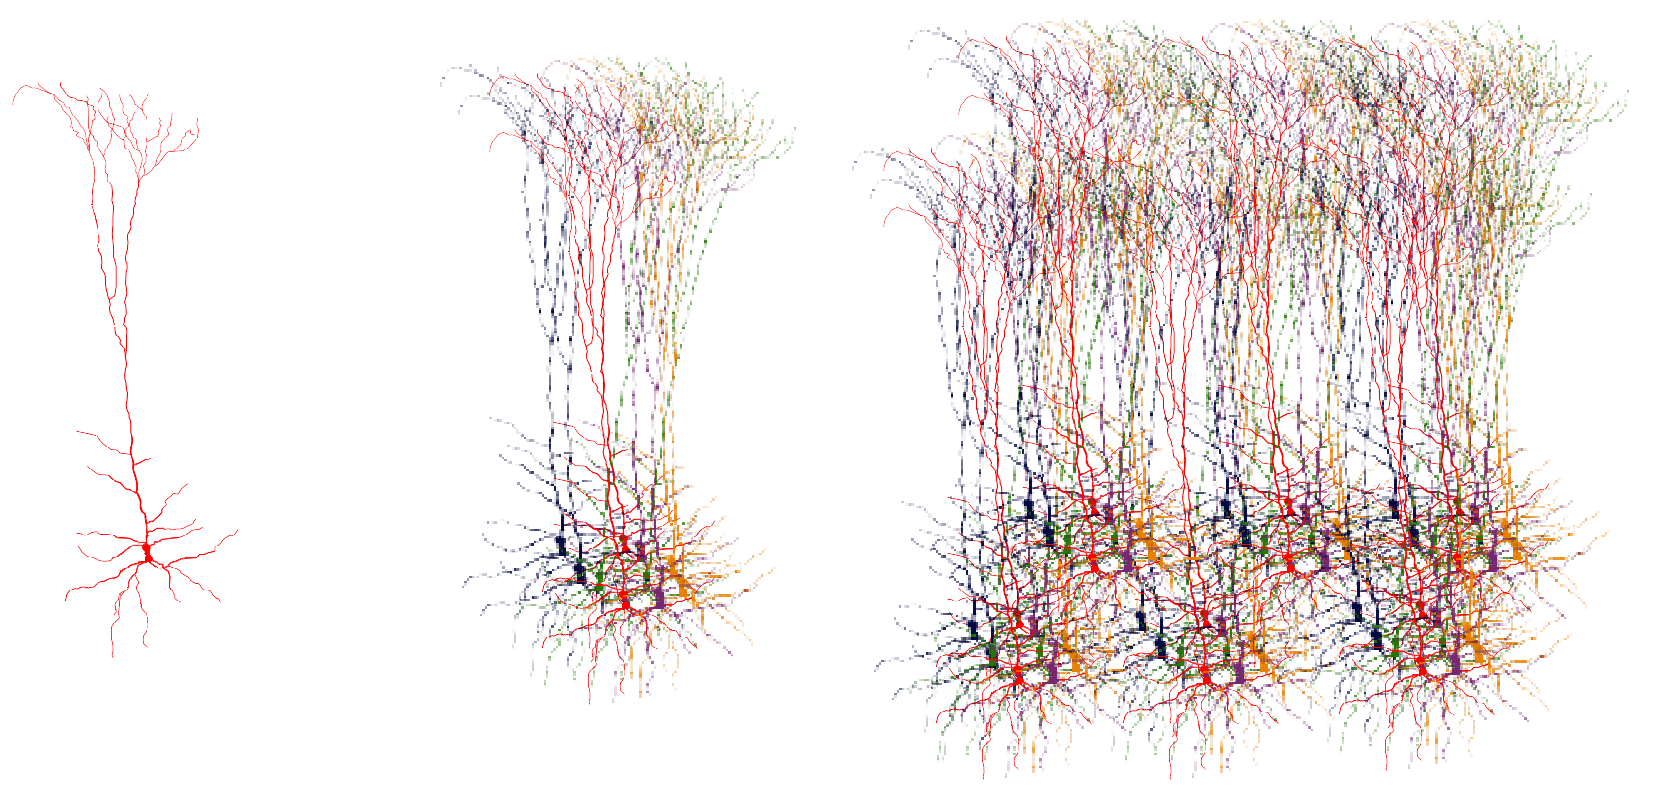
\includegraphics[width=1.0\textwidth]{Biological.png}
    \caption{Cortical tissue organization. Left: Pyramidal cell. The most common excitatory neuron in cortical tissue.
    Center: Cortical mini-column. A cluster on neural cells which responds to stimuli of similar characteristics.
    Right: Cortical Column. A group of mini-columns with a common receptive field location.
%    We use and modify and image whose author attribution is:
    Adapted from (Fabuio, Own work, CC BY 4.0, \url{https://commons.wikimedia.org/w/index.php?curid=60707501)}}
    \label{fig:Biological}
\end{figure}

According to recent findings in neuroscience,
%\emph{the brain uses \glspl{sdr} to process information}
\emph{the brain processes information by means of \glspl{sdr}}
\cite{barth_2012}.
This is true for all mammals, from mice to humans. Extended depolarization of the soma could be the result of independent dendritic \gls{nmda} branch activations produced by the excitation of certain number of distal synapses \cite{antic_2010, major_2013}. Adaptation to contextual stimuli is ubiquitous in cortical tissue and is thought to enhance efficiency in the codification of sensory information. By means of a reduction in the responses to frequent sounds, complex inhibitory networks may enhance cortical sensitivity to rare sounds that may represent unexpected events \cite{Natan2015ComplementaryCO,nachum_2003,Javitt11962}.

\subsection*{Model}
We propose a computational approach called \gls{cstm}, which simulates a patch of cortical tissue and incorporates columnar organization, spontaneous micro-columnar formation, and partial \gls{nmda} depolarization and adaptation to contextual activations. We simulate pyramidal cells with proximal connections from afferent dendritic branches and distal connections from lateral dendritic branches. Similar afferent stimuli activate clusters of neurons with proximal physical locations in a \gls{cc} in the same way that afferent information activates the mini columns found in cortical tissue.

Afferent information activates different clusters of units in a \gls{cc} establishing a first and raw approximation of the phonetic features abstracted from the input auditory stream. Our model fine-tunes such raw features by means of previous contextual activations produced in the same and/or in neighboring \glspl{cc}. Such contextual information is sent to each \gls{cc} by means of lateral distal dendritic branches which work as independent processing elements in a cell. Current activation in such dendritic elements will affect the way in which cells receives future afferent information.

Novel computational theories have posited a feasible explanation about the role of distal synapses related to \gls{nmda}
phenomenon \cite{hawkins_2016} by combining it with \glspl{sdr} \cite{ahmad_2016}. In our model, we adopt a similar approach to the one in \cite{hawkins_2016} in which current activation patterns produce partial depolarization of certain cells by means of distal dendritic branch connections. A state of partial depolarization is sustained in time in some cells within
future afferently excited clusters of neurons. Cells fire in advance with respect to other cells in the excited clusters, thereby preventing other cells from firing by means of proximal lateral GABAergic inhibition, obtaining in this way, \glspl{sdr}.

In addition, we simulate the growth of distal dendritic branch synapses by means of \gls{stdp} mechanisms together with
homeostatic regulations. In this way, distal synapses will be established only among pyramidal cells with sequential patterns
of activation. Afferently excited clusters which do not have partially depolarized cells,
will fire together producing a \gls{mfe}
(lack of inhibition) as a response to a prediction fault (unexpected sequential stimuli in the stream of data); otherwise they will respond with normal firing events (inhibition and therefore \glspl{sdr}) when the sequential stimulus is
correctly predicted.

\glspl{sdr} exhibit interesting mathematical properties which give them high noise rejection and fault tolerance \cite{ahmad_2015}.
%~\todo{Why?} ~\todo{This is a complex mathematical explanation which--I think--can not be summarized in few words. All the information is in the paper cited. I have read, understood and given talks about such paper here in Mendoza.}
These are typical characteristics in cortical tissue where individual cells are far from 100\% reliable and the cells die and regenerate continuously. To simulate this phenomenon, we incorporate stochastic characteristics by which neural cells inside afferently activated clusters are chosen to be active by a discrete distribution whose probabilities are determined by the afferent excitability of individual cells during training.

Hence, the evolution of our network does not predetermine a neuron to fire but biases its probability of doing so during training. Additionally, afferent dendritic arborizations activate themselves at random with levels whose boundary values are established by learning. 

%~\todo{by whom?} ~\todo{I have cited it at the end of the sentence George (\cite{JMLR:v15:srivastava14a})}
It has been shown that overfitting--a phenomenon in which a statistical model describes random error or noise instead of the underlying relationship--is greatly reduced by stochastic properties in training procedures applied to neural networks (dropout)~\cite{JMLR:v15:srivastava14a}.

In order to produce the inputs from auditory streams we follow  \gls{mrstsa}~\cite{chi_2005}. In our software implementation, we primarily follow its cortical section rather than its sub-cortical counterpart, incorporating different neurophysiological phenomena found in \gls{a1}~\cite{wang_1995} such as symmetry \cite{shamma_1993}, bandwidth \cite{schreiner_1990}, and frequency modulation selectivity \cite{shamma_1993,heil_1992,mendelson_1985}.

\subsection*{Experiments}

We test the phonetic feature invariance capacity of our cortical model--in a stage called \gls{el}-- 
%inside the \gls{cstm}--
in several word classification tasks. We compare its performance with the performance of the features returned by the \gls{mrstsa} algorithm by means of \gls{svm} classification of features delivered by each algorithm (Fig. \ref{fig:Experiment}).

\begin{figure}[h!]
    \centering
    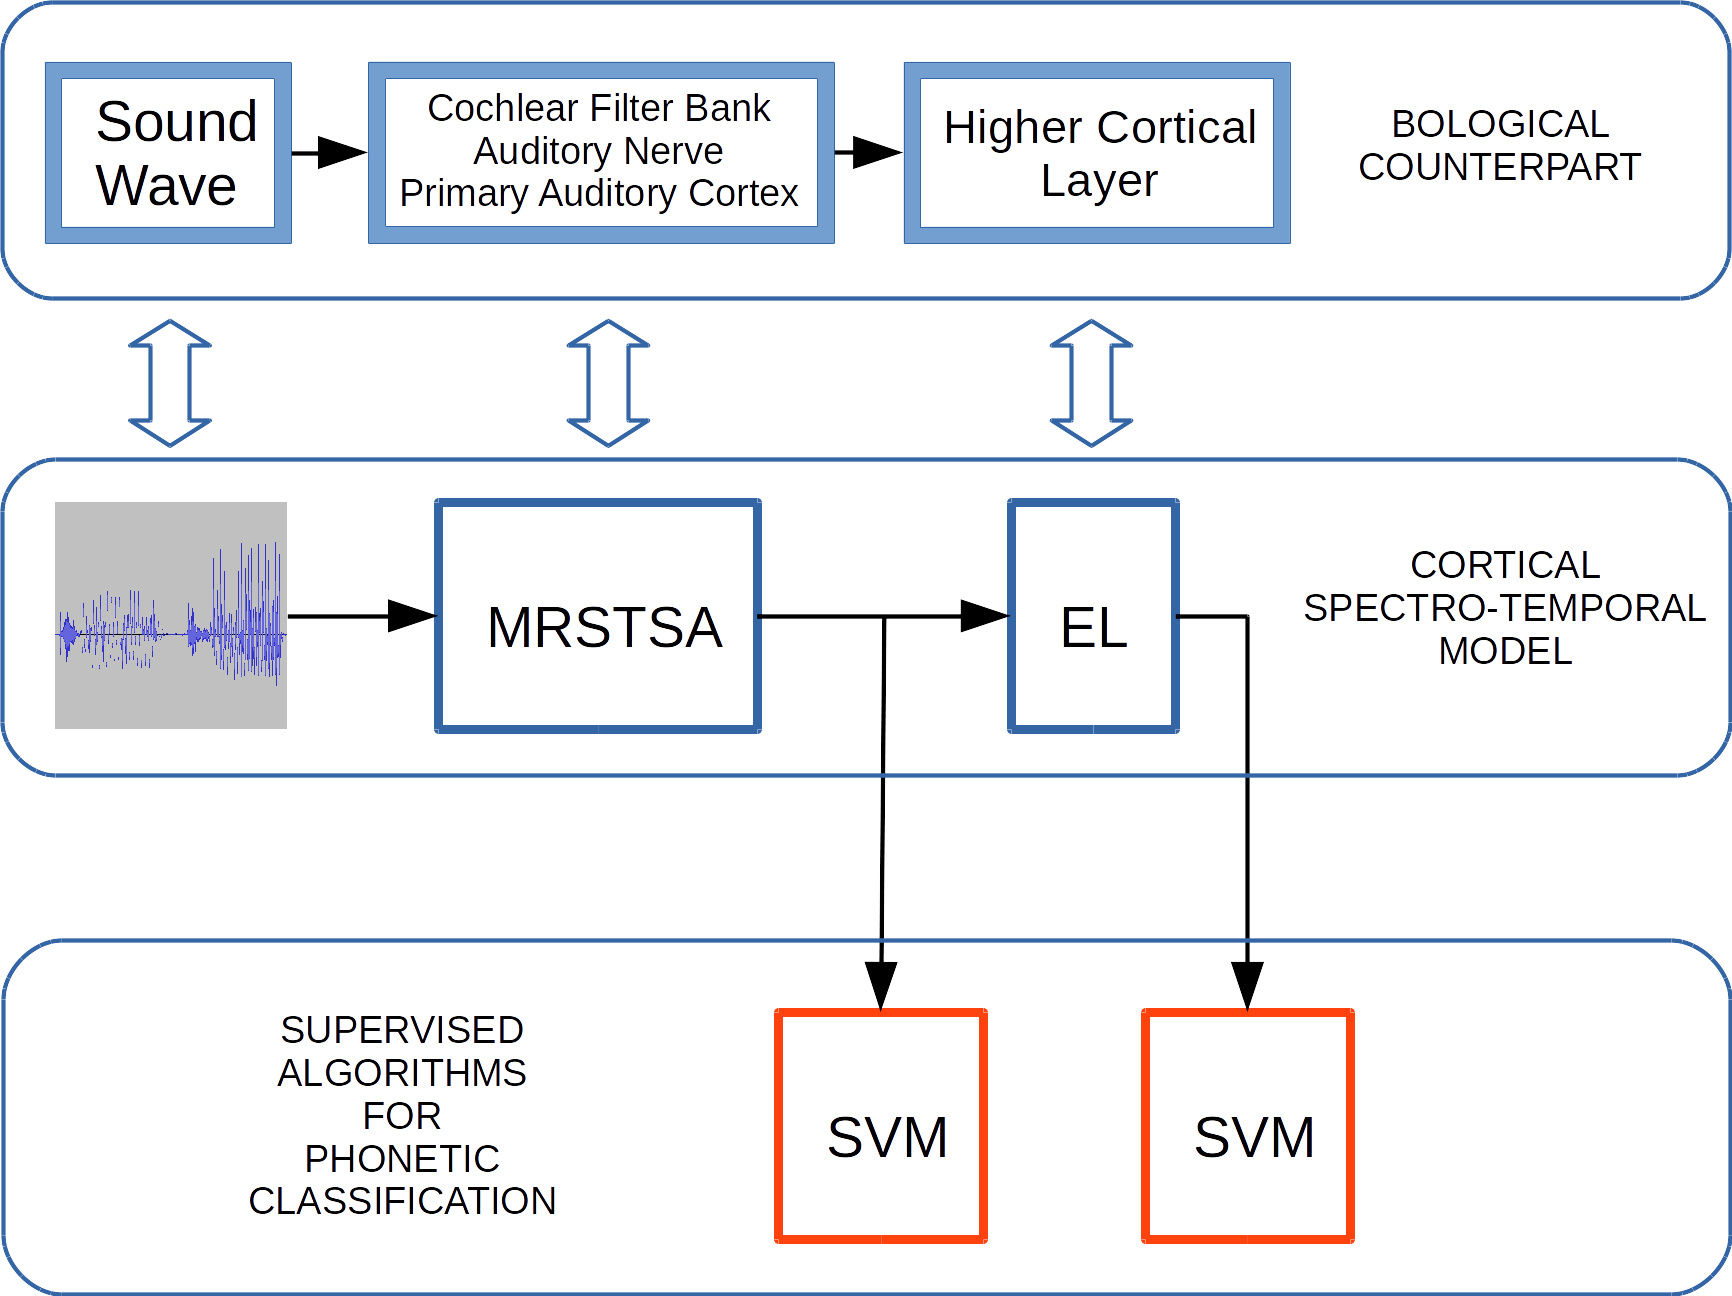
\includegraphics[width=0.8\textwidth]{Experiment.png}
    \caption{Experimental setup to test word classification task performances.
    Sound waves are processed by the \gls{mrstsa} algorithm.
    The outputs from the \gls{mrstsa} are processed by the \gls{el}.
    Word classification tasks are performed on both outputs by the \gls{svm} algorithm.
    Each section in the \gls{cstm} has its biological counterpart.}
    \label{fig:Experiment}
\end{figure}

\pagebreak

We demonstrate via a computational simulation that our implementation of the cortical model leverages the performance in word classification tasks under certain environmental conditions (e.g., white noise and reverberation) and for certain variances applied to the auditory stimuli (e.g., pitch variations). We also demonstrate effectiveness in classifying multisyllabic words, which suggests that our implementation of neurophysiological predictive dynamics plus stochastic sparse patterns of activation outperforms the \gls{mrstsa} algorithm in terms of phonotactic sequential invariance for disturbances applied to the audio signal. 

Given these promising results, we posit that neurophysiological and anatomical properties in our model are potentially relevant to the design of artificial intelligence systems and may achieve higher levels of phonetic invariance and generalization than the ones achieved by current deep learning architectures.

% NOTE FROM GEORGE
% Editing completed to here on Sunday, May 6.
% end of our old introduction


























\section*{Computational Model}

We introduce a computational model called \textbf{\glsfirst{cstm}}. The \gls{cstm} consists of two parts: The \glsfirst{el} and the \glsfirst{mrstsa}. 

The \glsfirst{el} converts a multidimensional array of real numbers into a multidimensional \gls{sdr}.
This stage 
%is composed by 
consists of
a set of \glspl{som} \cite{kohonen_2082, Kohonen:1989:SAM:69371}
and incorporates neurophysiological phenomena such as columnar organization, afferent spontaneous
micro-columnar formation, proximal and distal dendritic arborization, lateral intercolumn interaction by means of independent dendritic \gls{nmda} branch activations, \glspl{mfe} with contextual stimulus adaptation, proximal lateral intracolumn inhibition, \gls{ltp}, \gls{ltd}, \gls{stdp} and distal synaptic homeostatic regulations.

% Finally, 

The algorithm, \glsfirst{mrstsa}, processes the sound waves to feed inputs to the \gls{el}, a technique that is inspired by Chi T. et al. \cite{chi_2005}.
In our \gls{mrstsa} implementation, we follow main guidelines from the higher cortical representations
developed in \cite{chi_2005}.


% GKT Note: I reworked the following into the above. 
%In order to obtain the inputs 
%with which 
%to feed the encoder,
%we implemented an algorithm called \glsfirst{mrstsa}.
%We process the sound waves with such algorithm
%that takes guidelines from
%the technique elaborated 
%which is inspired 
%by Chi T. et al. \cite{chi_2005}
%In such work, accumulating experimental findings
%from the central auditory system
%were exploited demonstrating its applications in the objective
%evaluation of speech intelligibility.
%As the authors pointed out, the model was not biophysical in spirit,
%but rather it abstracted from the physiological data an interpretation
%which was likely to be relevant in the design of sound engineering systems.

\subsection*{\glsfirst{el}}

The \gls{el} is responsible for generating \glspl{sdr} from the inputs delivered by the \gls{mrstsa} stage
described in section \nameref{sec-mrstsa} and from the activation history in its own \glspl{cc}.

The \gls{el} simulates a patch of cortical tissue called \gls{cl}using an n-dimensional array of complex structures called \glspl{csom} that simulate \glspl{cc} in the brain.

Each \gls{cc} in the \gls{el} is connected to the \gls{mrstsa} below by means of afferent connections. It is also
connected to neighboring \glspl{cc}--including possibly itself--in the \gls{el} by means of lateral connections and
to \glspl{cc} from other \glspl{cl} above by means of apical connections. Such connection scheme is shown in Fig \ref{fig:EncoderColumnConnections}.

\begin{figure}[h!]
    \centering
    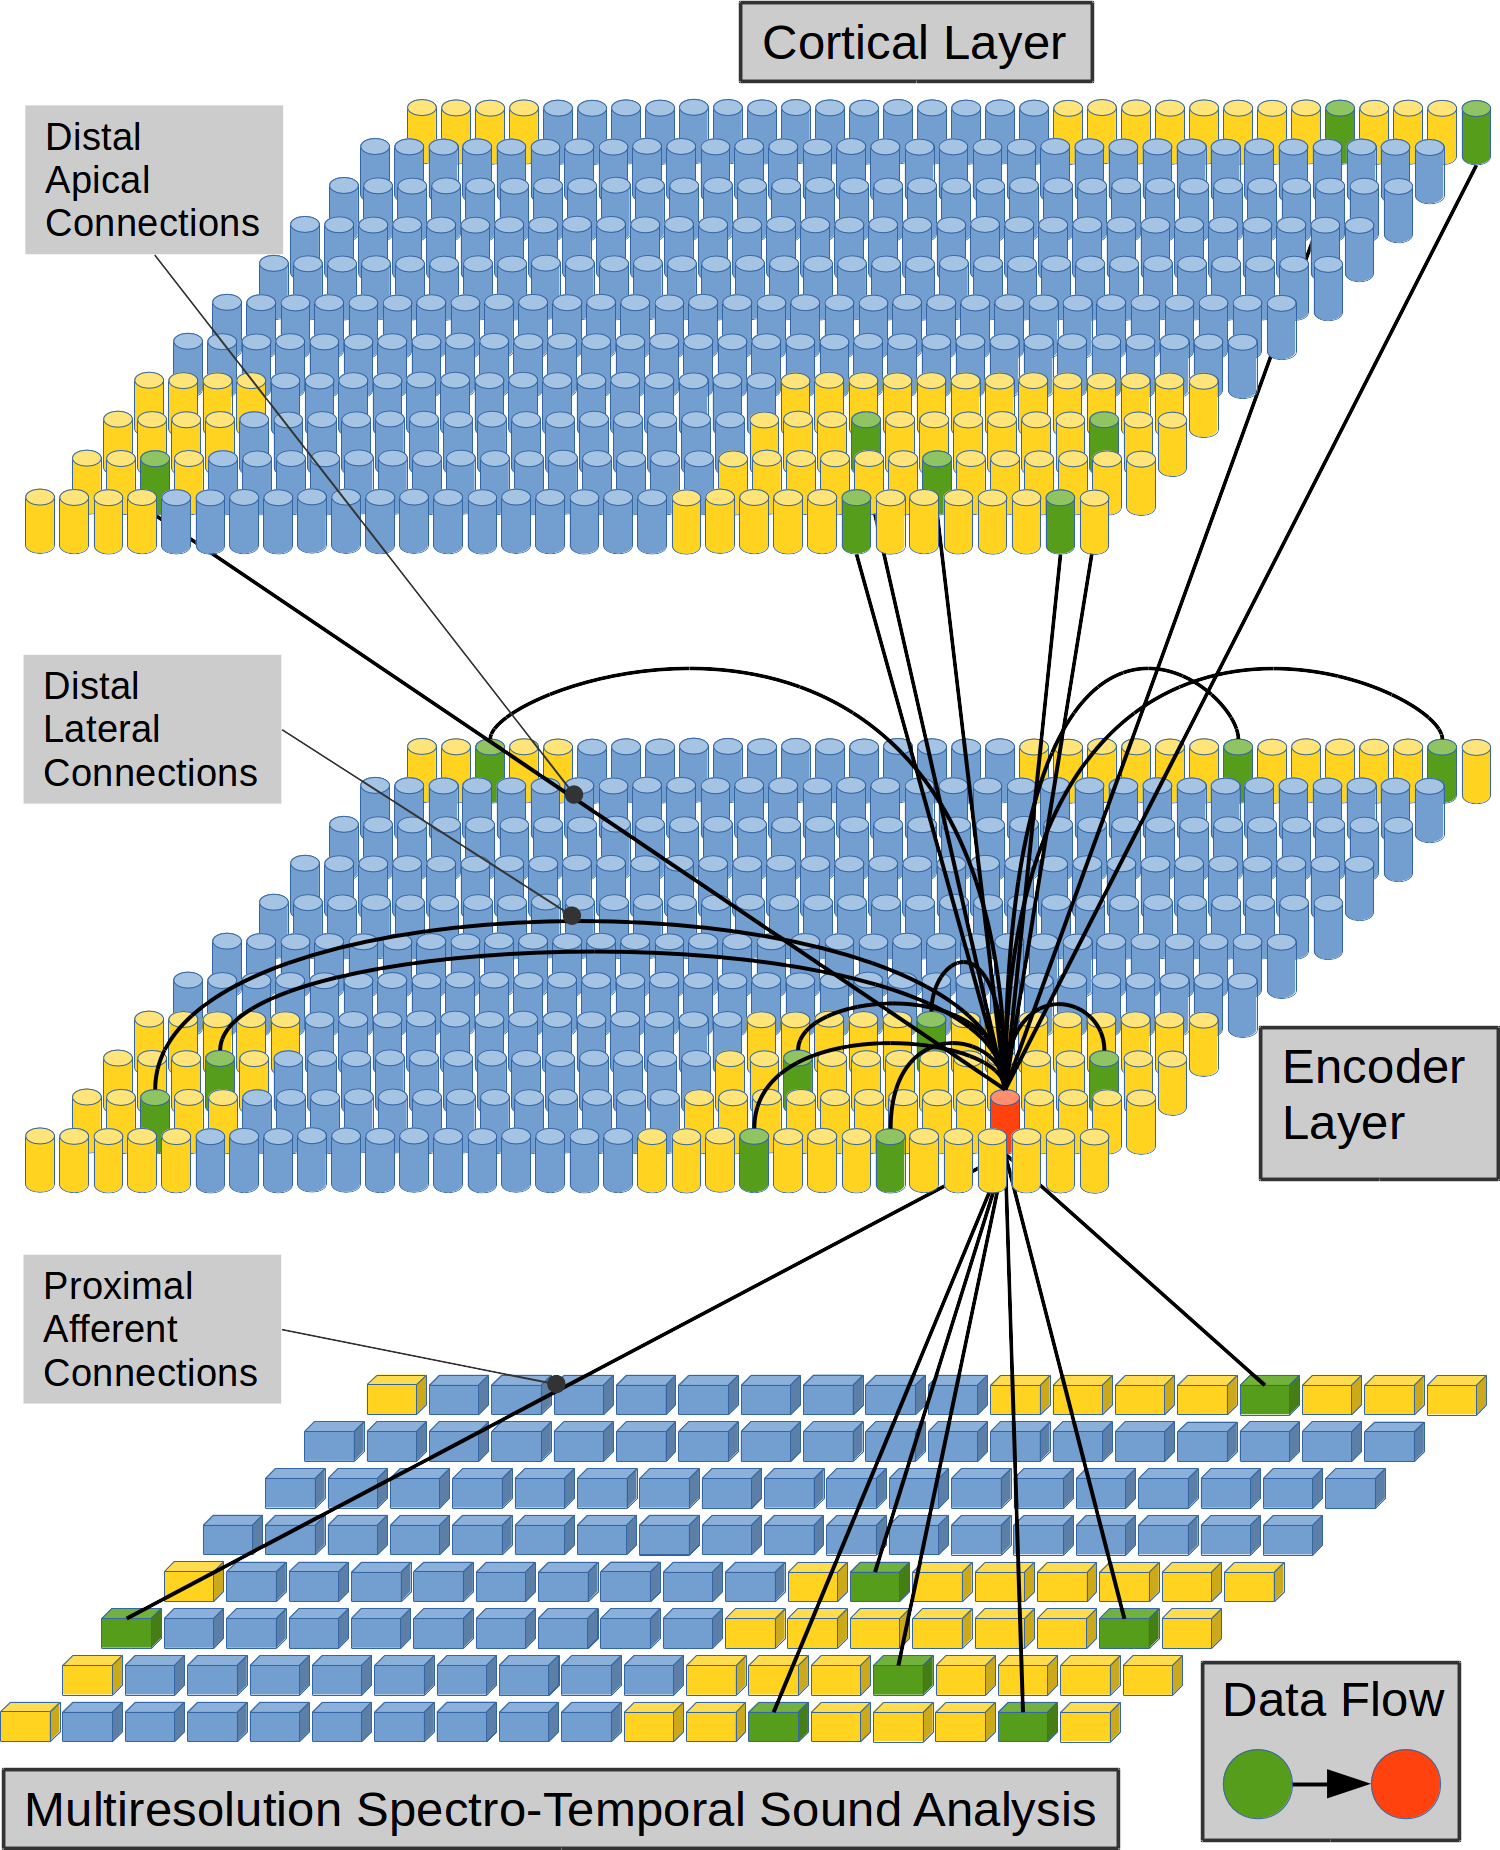
\includegraphics[width=0.6\textwidth]{EncoderColumnConnections.png}
    \caption{Connection scheme for a cortical column in the Encoder Layer.
	    Each cylinder in the \gls{el} and in the \gls{cl} represents a \gls{cc} in neural tissue.
	    Each prism in the \gls{mrstsa} represents a real valued variable.
	    This is a visualization of a \gls{cc} (in red) and its three receptive fields (in yellow).
	    The receptive field of a \gls{cc} is an array that defines a set of \glspl{cc}
	    with which such column could be connected.
	    The receptive field of a \gls{cc} on the \gls{mrstsa} determines an array of real valued variables
	    with which such column could be connected.
    A subset of \glspl{cc} in a receptive field (in green) represents the \glspl{cc} that are really
    connected with the \gls{cc} in red. A similar scenario could be described for the green prisms on
    the \gls{mrstsa}.
    The size, wrap-around property and percentage of established links (in green) inside a receptive field are tunable parameters for the model.
    In this work, only lateral connections have been implemented since in the current implementation there are no upper cortical layers from which
    to bring apical connections.}
    %Every neural unit in a \gls{cc} in the \gls{el} receives the same set of proximal connections from
    %the \gls{mrstsa}.
    %Such connections are modified following the statistical distribution from the \gls{mrstsa}
    %by means of the \gls{som} algorithm.}
    \label{fig:EncoderColumnConnections}
\end{figure}

\pagebreak


\iffalse
\begin{figure}[h!]
    \centering
    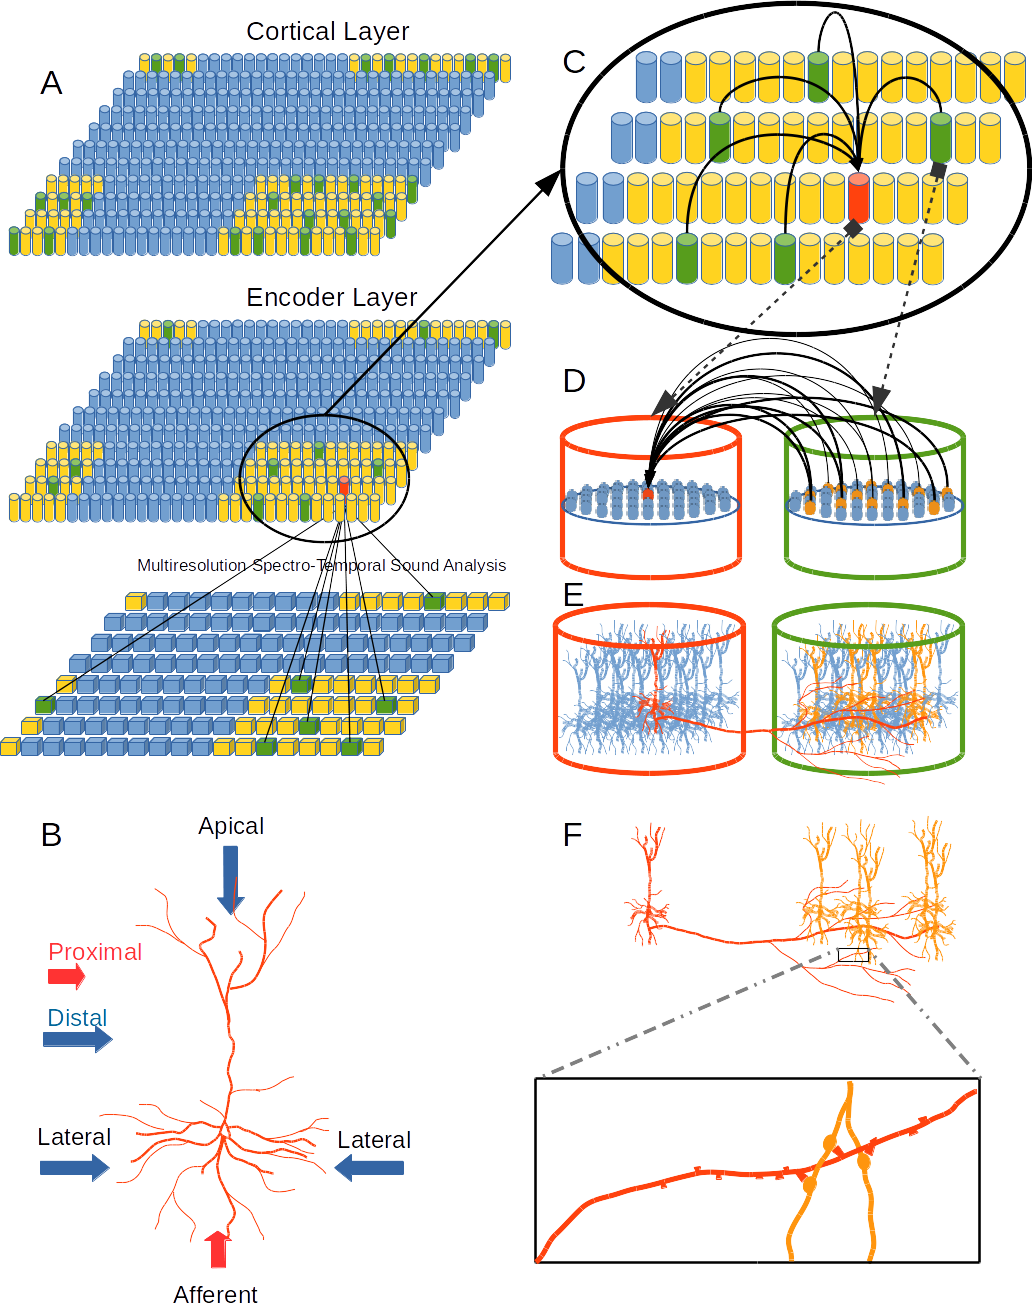
\includegraphics[width=0.9\textwidth]{Connectivity.png}
    \caption{\tiny Connection scheme for a cortical column in the Encoder Layer.
	    (A) Each cylinder in the \gls{el} and in the \gls{cl} represents a \gls{cc} in neural tissue.
	    Each prism in the \gls{mrstsa} represents a real valued variable.
	    This is a visualization of a \gls{cc} (in red) and its three receptive fields (in yellow).
	    The receptive field of a \gls{cc} is an array that defines a set of \glspl{cc}
	    with which such column could be connected.
	    The receptive field of a \gls{cc} on the \gls{mrstsa} determines an array of real valued variables
	    with which such column could be connected.
    A subset of \glspl{cc} in a receptive field (in green) represents the \glspl{cc} that are really
    connected with the \gls{cc} in red. A similar scenario could be described for the green prisms on
    the \gls{mrstsa}.
    The size, wrap-around property and percentage of established links (in green) inside a receptive field are tunable parameters for the model.
    Every neural unit in a \gls{cc} in the \gls{el} receives the same set of proximal connections from
    the \gls{mrstsa}.
    Such connections are modified following the statistical distribution from the \gls{mrstsa}
    by means of the \gls{som} algorithm.
    (B) Connectivity profile of a pyramidal neural unit in the \gls{el}.
    Proximal connections are formed only by afferent connections from the \gls{mrstsa}
    while distal connections are formed by lateral and apical connections from neighboring columns and
    from columns in another cortical layer above respectively.
    (C) Distal dendritic branches from neighboring \glspl{cc} inside the receptive field
    of a \gls{cc} in the \gls{el}. A distal dendritic branch between the red \gls{cc} and a
    green \gls{cc} means that every neural unit in the red \gls{cc} is linked with a different
    subset of neural units in the green \gls{cc} by means of potential connections.
    (D) Potential connections in a dendritic branch which link a neural unit in the red \gls{cc}
    with a subset of neural units in a green \gls{cc}. The subset of potential connections comes from a percentage of neural units
    inside the green \gls{cc}. Such percentage is a tunable parameter for the \gls{cc}.
    (E) A distal dendritic branch between a pyramidal cell in a \gls{cc} and a 
    sub-set of pyramidal cells in a neighboring \gls{cc} inside its receptive field
    in the \gls{el}.
    (F) Physical proximity of a dendritic branch from the red cell to axonal branches from yellow cells constitutes potential connections
    which could prosper becoming in established synapses depending on the sequential activity among cells.}
    \label{fig:Connectivity}
\end{figure}
\fi

Both lateral and apical are feedback connections that constitute contextual information channels. 
These channels put the current afferent excitation under the context of previous activations.
Such connections damp the activity of some units allowing only the precise activations
of specific neural units in an afferently excited \gls{cc}.
Such precise activations match the sequential paradigms learned by the network.

Recent findings in neuroscience \cite{Marques2018} support the idea 
that feedback could potentially enhance visual representations in time and space
damping the activity of certain cells while allowing the 
%activations  
activation
of others
%which agree 
in agreement
with its predictions.

In this paper we only implement lateral connections since
there are no upper layers 
from which to bring apical information in the present implementation.

Each cell unit in a \gls{cc} has two types of dendritic branches; proximal and distal.
Proximal and distal dendritic branches lead to proximal and distal connections in a cell unit respectively.
Proximal and distal connections produce different effects on a neural unit's plasticity and activation.
Neural units in the \gls{el} simulates pyramidal cells in cortical tissue in the brain.
Fig \ref{fig:PyramidalCell} shows the connectivity profile in such units. 

\begin{figure}[h!]
    \centering
    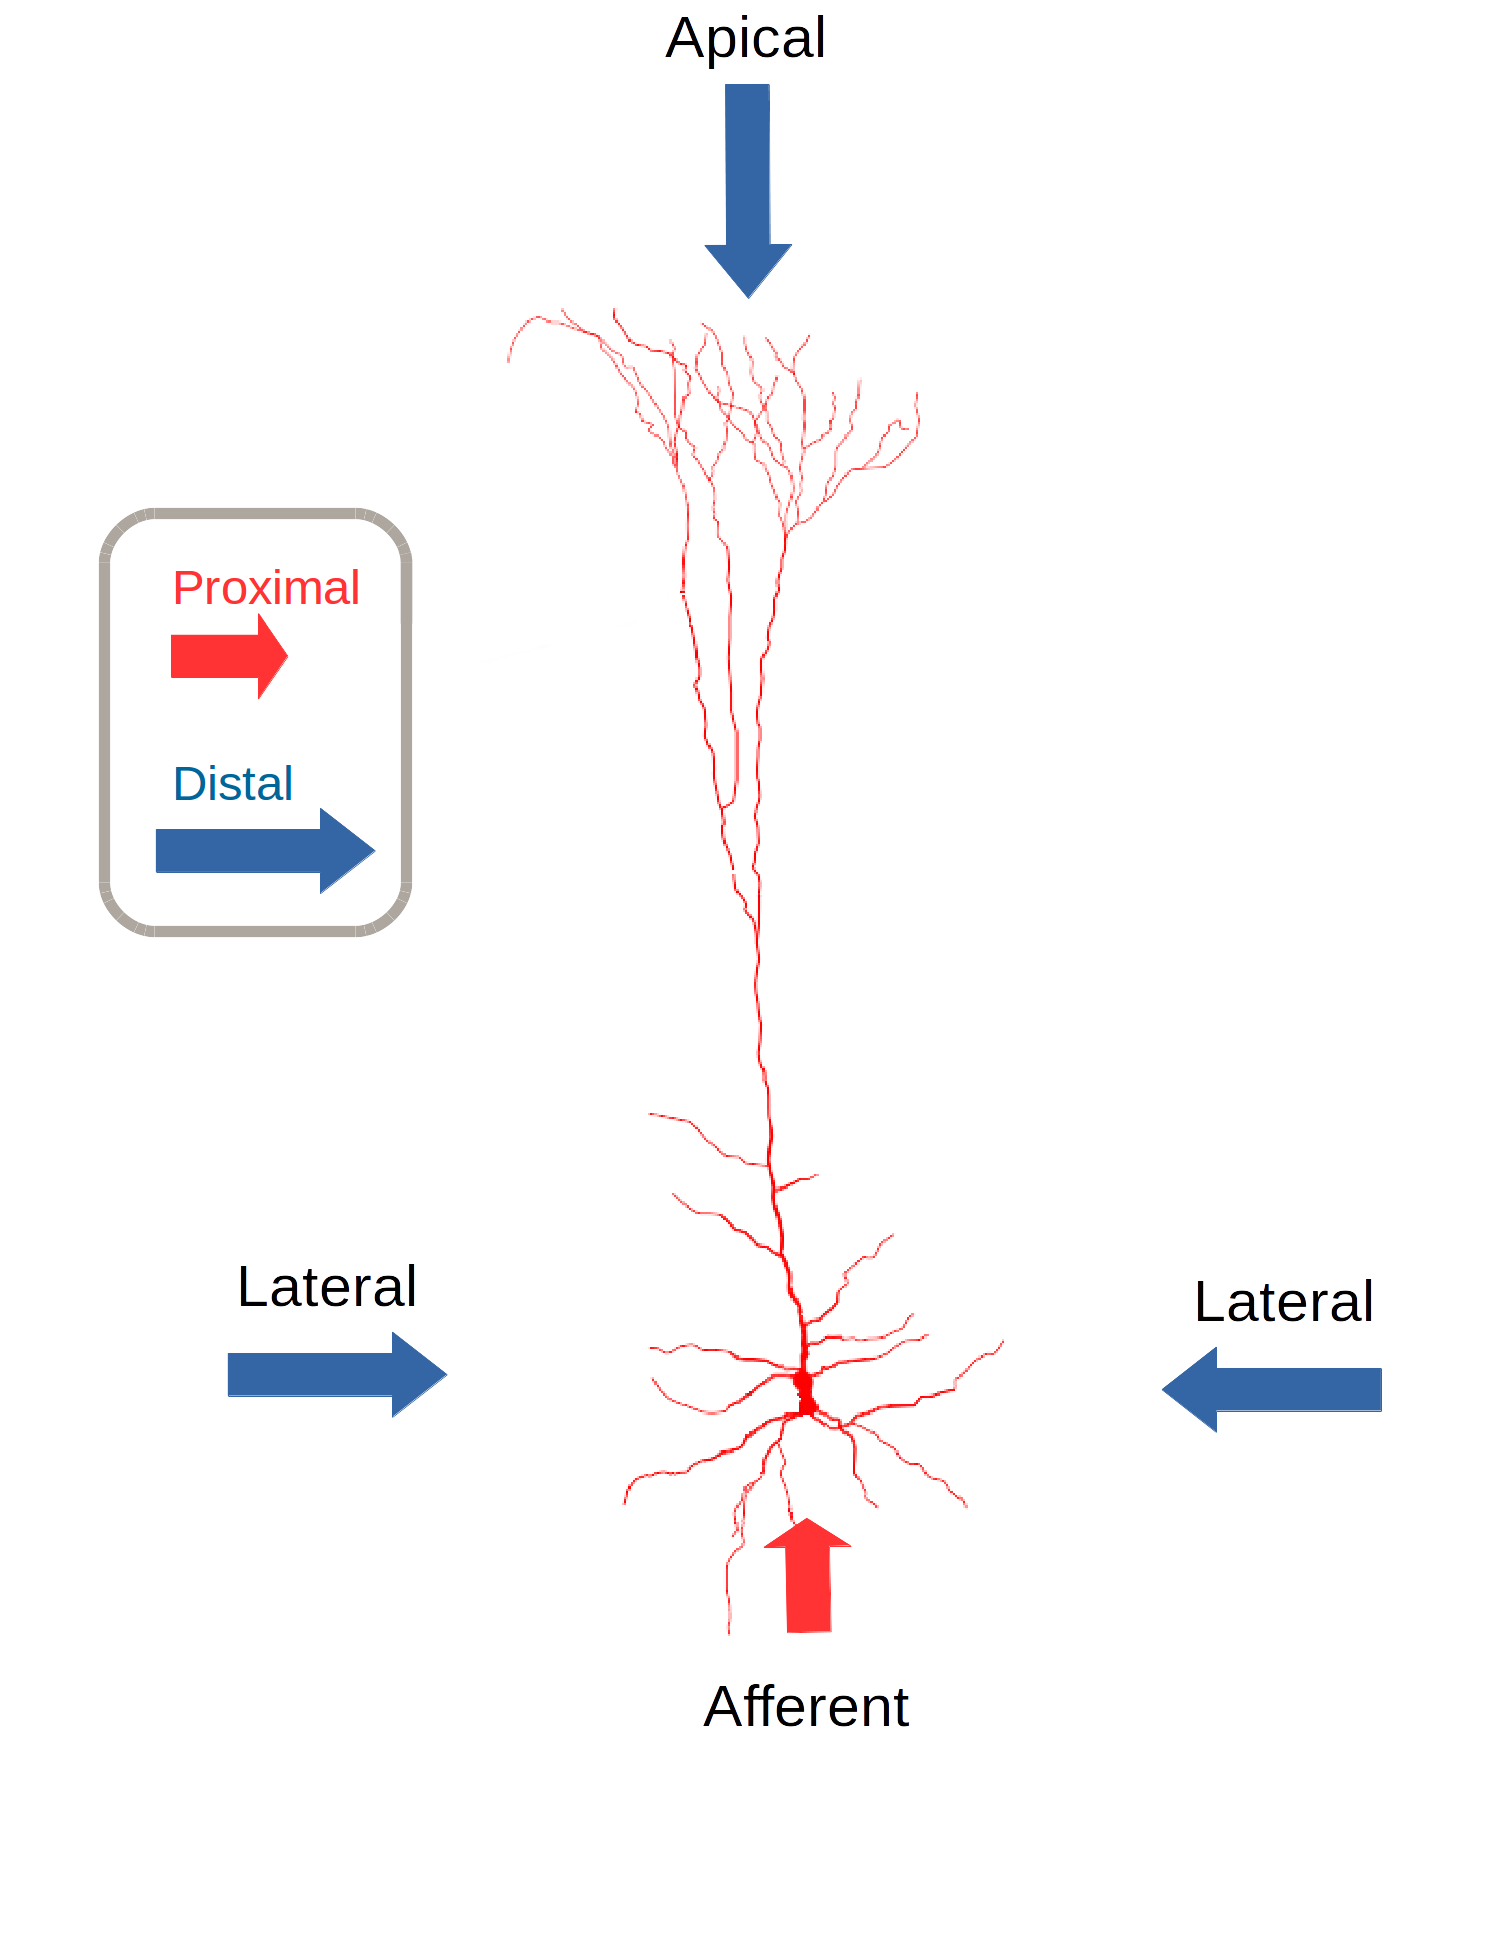
\includegraphics[width=0.9\textwidth]{PyramidalCell.png}
    \caption{Connectivity profile of a pyramidal neural unit in the \gls{el}.
    Proximal connections are formed only by afferent connections from the \gls{mrstsa}
    while distal connections are formed by lateral and apical connections from neighboring columns and
    from columns in another cortical layer above respectively.
    Adapted from 
    (Fabuio - Own work, CC BY 4.0, \url{https://commons.wikimedia.org/w/index.php?curid=60707501)}}
    \label{fig:PyramidalCell}
\end{figure}

\pagebreak

\subsubsection*{Proximal dendritic connections}

In reference to proximal connections in the \gls{el}, each neural unit in a \gls{cc} has the same set of
proximal connections to the \gls{mrstsa} (Fig \ref{fig:EncoderColumnConnections}).
Such connections constitute a multidimensional space of real numbers.
In order to acquire the statistical distribution in such multidimensional real space we use
a multidimensional \gls{som} in each cortical column.

A \gls{som} is an unsupervised clustering algorithm which distributes a continuous multidimensional distribution
in a discrete multidimensional distribution of units \cite{Kohonen:1989:SAM:69371, kohonen_2082}.
In this way we ended up with an array of units of $m$ dimensions in which each unit
represents a set of vectors from the continuous distribution in an input space of $n$ dimensions.
Generally, $m < n$ in order to reduce the dimensionality in the discrete representation.
We added such restriction in our columnar algorithm.

In the \gls{som} algorithm, each input vector has to be completely determined.
In our case, some inputs from the \gls{mrstsa} could be null,
and each input vector could not have the information of each of its components available.
We incorporated a stochastic mechanism in the \gls{el} in order to deal with such situation.
We made each afferent connection to learn statistical boundaries from its corresponding input.
We establish a minimum-maximum margin in each proximal connection in the \gls{el}.
Such margin is consistent with the statistical distribution in the history of its corresponding input.
When an afferent input is undetermined, in a context in which some afferent inputs have
available information,
the \gls{el} chooses
the value in the undetermined input
%is chosen
randomly
between the boundaries learned for such input.

We call our implementation of the \gls{som} algorithm, \gls{ssom}.
The \gls{ssom} algorithm accounts for proximal lateral intra-column interaction, \gls{ltp} and
\gls{ltd}.
It also dissociates proximal dendritic inputs from distal dendrites, since
it modifies
proximal connections
%are modified
following the statistical distribution from the
\gls{mrstsa} independently of the units that fire in such \gls{cc}.
This independence in the plasticity of the proximal dendritic inputs
%uses
is supported by
the
%fact
property
found in cortical tissue by means of which there is dendritic plasticity
in the context of partial depolarization of the soma \cite{reiter_1998}--that is, without an \gls{ap}. % Citation needed here

The term \textit{static} comes from the fact that the patterns learned from proximal afferent
dendrites do not account for the contextual history in the dynamic evolution
of the algorithm.








\subsubsection*{Distal dendritic connections}

In terms of distal dendritic branches, each \gls{cc} in the \gls{el} is connected to other \glspl{cc}--in green in Fig \ref{fig:EncoderColumnConnections}--by means of such
branches inside the receptive fields--in yellow in Fig. \ref{fig:EncoderColumnConnections}--from the same \gls{el} and from another \gls{cl}
above.
Each link between the red \gls{cc} and a green \gls{cc}--Fig. \ref{fig:DistalDendrites} A--
symbolizes the fact that each cell unit in
the red \gls{cc} is linked with a different subset of cell units in the green \gls{cc}--Fig. \ref{fig:DistalDendrites} B.

\begin{figure}[h!]
    \centering
    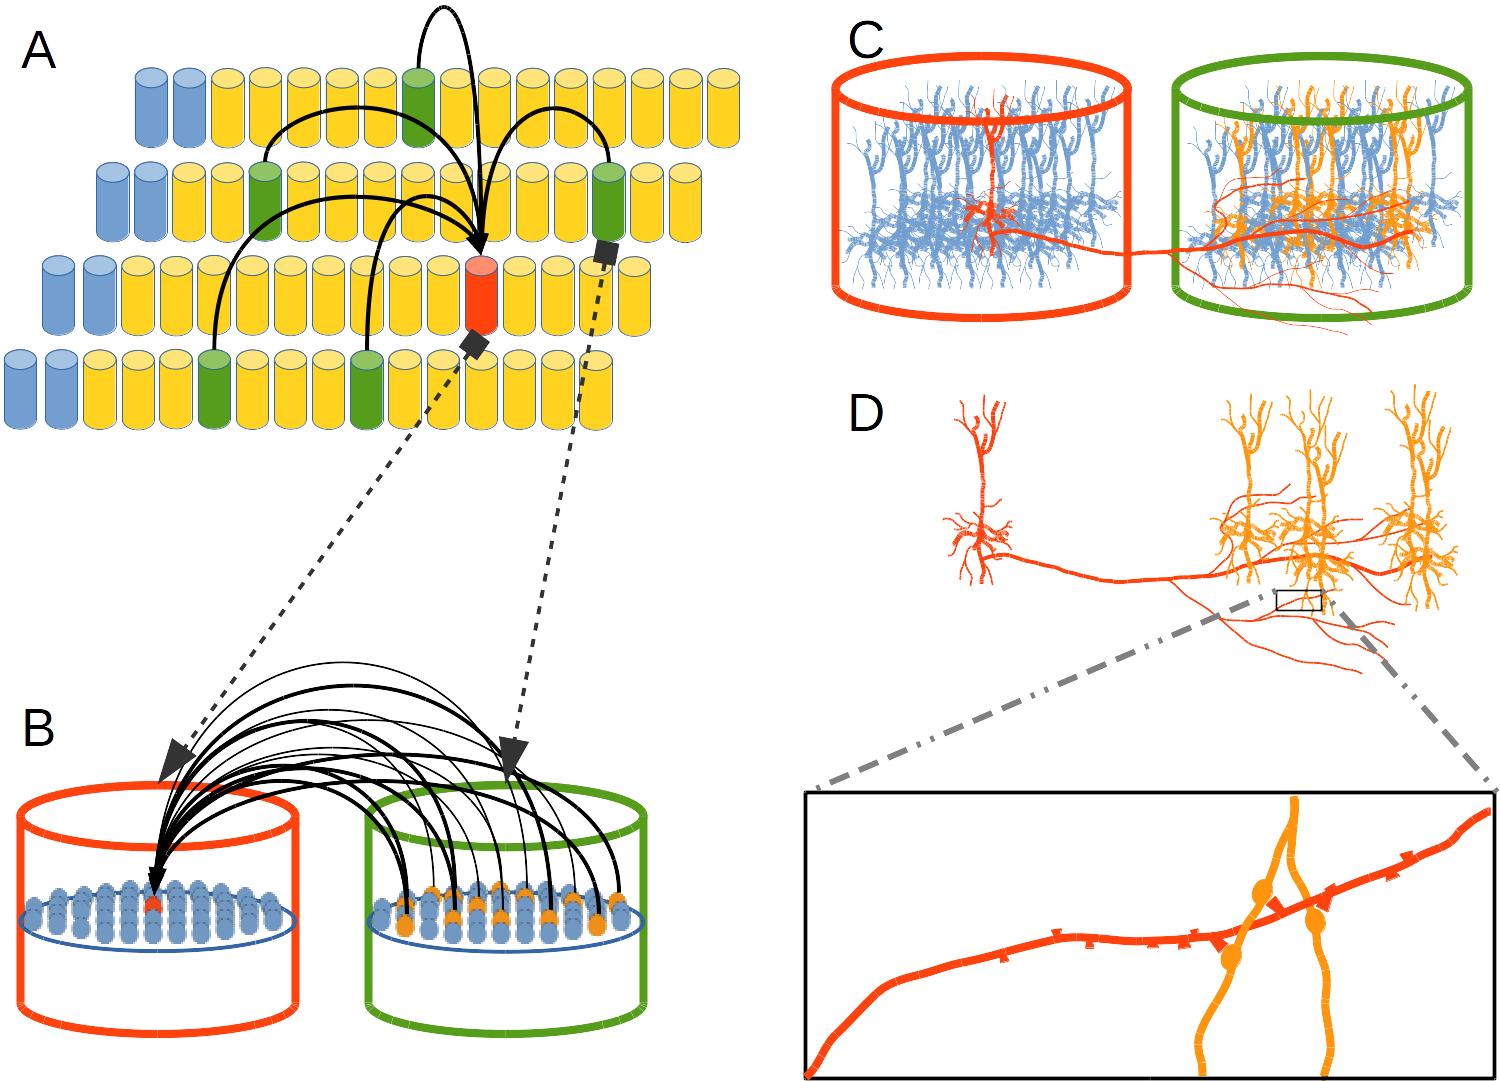
\includegraphics[width=0.9\textwidth]{DistalDendrites.png}
    \caption{Distal dendrite connections. (A) Distal dendritic branches from neighboring \glspl{cc} inside the receptive field
    of a \gls{cc} in the \gls{el}. A distal dendritic branch between the red \gls{cc} and a
    green \gls{cc} means that every neural unit in the red \gls{cc} is linked with a different
    subset of neural units in the green \gls{cc} by means of potential connections.
    (B) Potential connections in a dendritic branch which link a neural unit in the red \gls{cc}
    with a subset of neural units in a green \gls{cc}. The subset of potential connections comes from a percentage of neural units
    inside the green \gls{cc}. Such percentage is a tunable parameter for the \gls{cc}.
    (C) A distal dendritic branch between a pyramidal cell in a \gls{cc} and a 
    sub-set of pyramidal cells in a neighboring \gls{cc} inside its receptive field
    in the \gls{el}.
    (D) Physical proximity of a dendritic branch from the red cell to axonal branches from yellow cells constitutes potential connections
    which could prosper becoming in established synapses depending on the sequential activity among cells.}
    \label{fig:DistalDendrites}
\end{figure}

\pagebreak

Such links in Fig \ref{fig:DistalDendrites} A, represent dendritic branches in neural tissue and
we call
each connection in Fig. \ref{fig:DistalDendrites} B,
%is called
potential connection.
%and
Potential connections represent synapses in the dendritic branch.
A cell unit inside the red \gls{cc} ends up with as many dendritic branches as green \glspl{cc} inside its receptive field (Fig \ref{fig:DistalDendrites} A.)

The term \emph{potential connection} is used, because it describes a pair of neural units linked by its physical location and dendritic and axonal disposition in cortical tissue (Fig. \ref{fig:DistalDendrites} C). However, an effective connectivity between such neurons will depend upon their sequential pattern of activation which will establish developed synapses between them. If two neural units--a red one and a yellow one in Fig. \ref{fig:DistalDendrites} D--are linked by means of a distal potential connection--produced by a synapse between a distal dendritic branch from the red one and an axonal branch from the yellow one--such connection will grow only if there is a sequential activation of the red cell after an activation of the yellow cell, in two consecutive time steps. If such phenomenon does not repeat itself over time, such synapse will decrease its strength with respect to other synapses in the dendritic branch in the red cell in Fig. \ref{fig:DistalDendrites} D. A simultaneous activation in both neural units--the red one and the yellow one in Fig. \ref{fig:DistalDendrites} D--will decrease the strength in such potential connection.

We implemented distal dendritic synaptic plasticity mechanisms by means of an algorithm called \gls{dsom}.
The learning mechanisms implemented on such algorithm simulate neurophysiological phenomena
such as \gls{stdp}, and homeostatic regulation plasticity in the synaptic strength regulation in
distal dendritic branches.







\subsubsection*{Activation rules in a \gls{cc}}

Finally, in reference to the activation rules of neural units inside a \gls{cc} in the \gls{el},
first a group of cell units in a \gls{cc} is partially depolarized 
by distal connections among such neural units and cell units activated in the
previous time step in the \gls{el}--Fig. \ref{fig:Activation} A.
That is, neural units activated in time step $t=0$ in the \gls{el}, will partially depolarize
a set of neural units in time step $t=1$ in such \gls{cc}, by means of distal--lateral and apical--
dendritic branch synapses established by learning in the \gls{dsom} algorithm.

Second, afferent proximal connections from \gls{mrstsa} will tend to depolarize
certain clusters of units in such \gls{cc} in time step $t=1$--Fig. \ref{fig:Activation} B.
The tentative depolarization is produced by the inputs from the \gls{mrstsa} with
proximal synapses established by learning in the \gls{ssom} algorithm. 
Such group of neural units are randomly chosen from a discrete distribution
whose probabilities are established by the state of excitation in afferent inputs.

If a sufficient number of partially depolarized units are in the set of
afferently excited units, such partially depolarized units
will fire previously in the group--Fig. \ref{fig:Activation} B left.
Those units--which fire before--prevent neighboring units in the excited clusters from firing,
hyperpolarizing them by means of lateral inhibitory connections in the column.

\begin{figure}[h!]
    \centering
    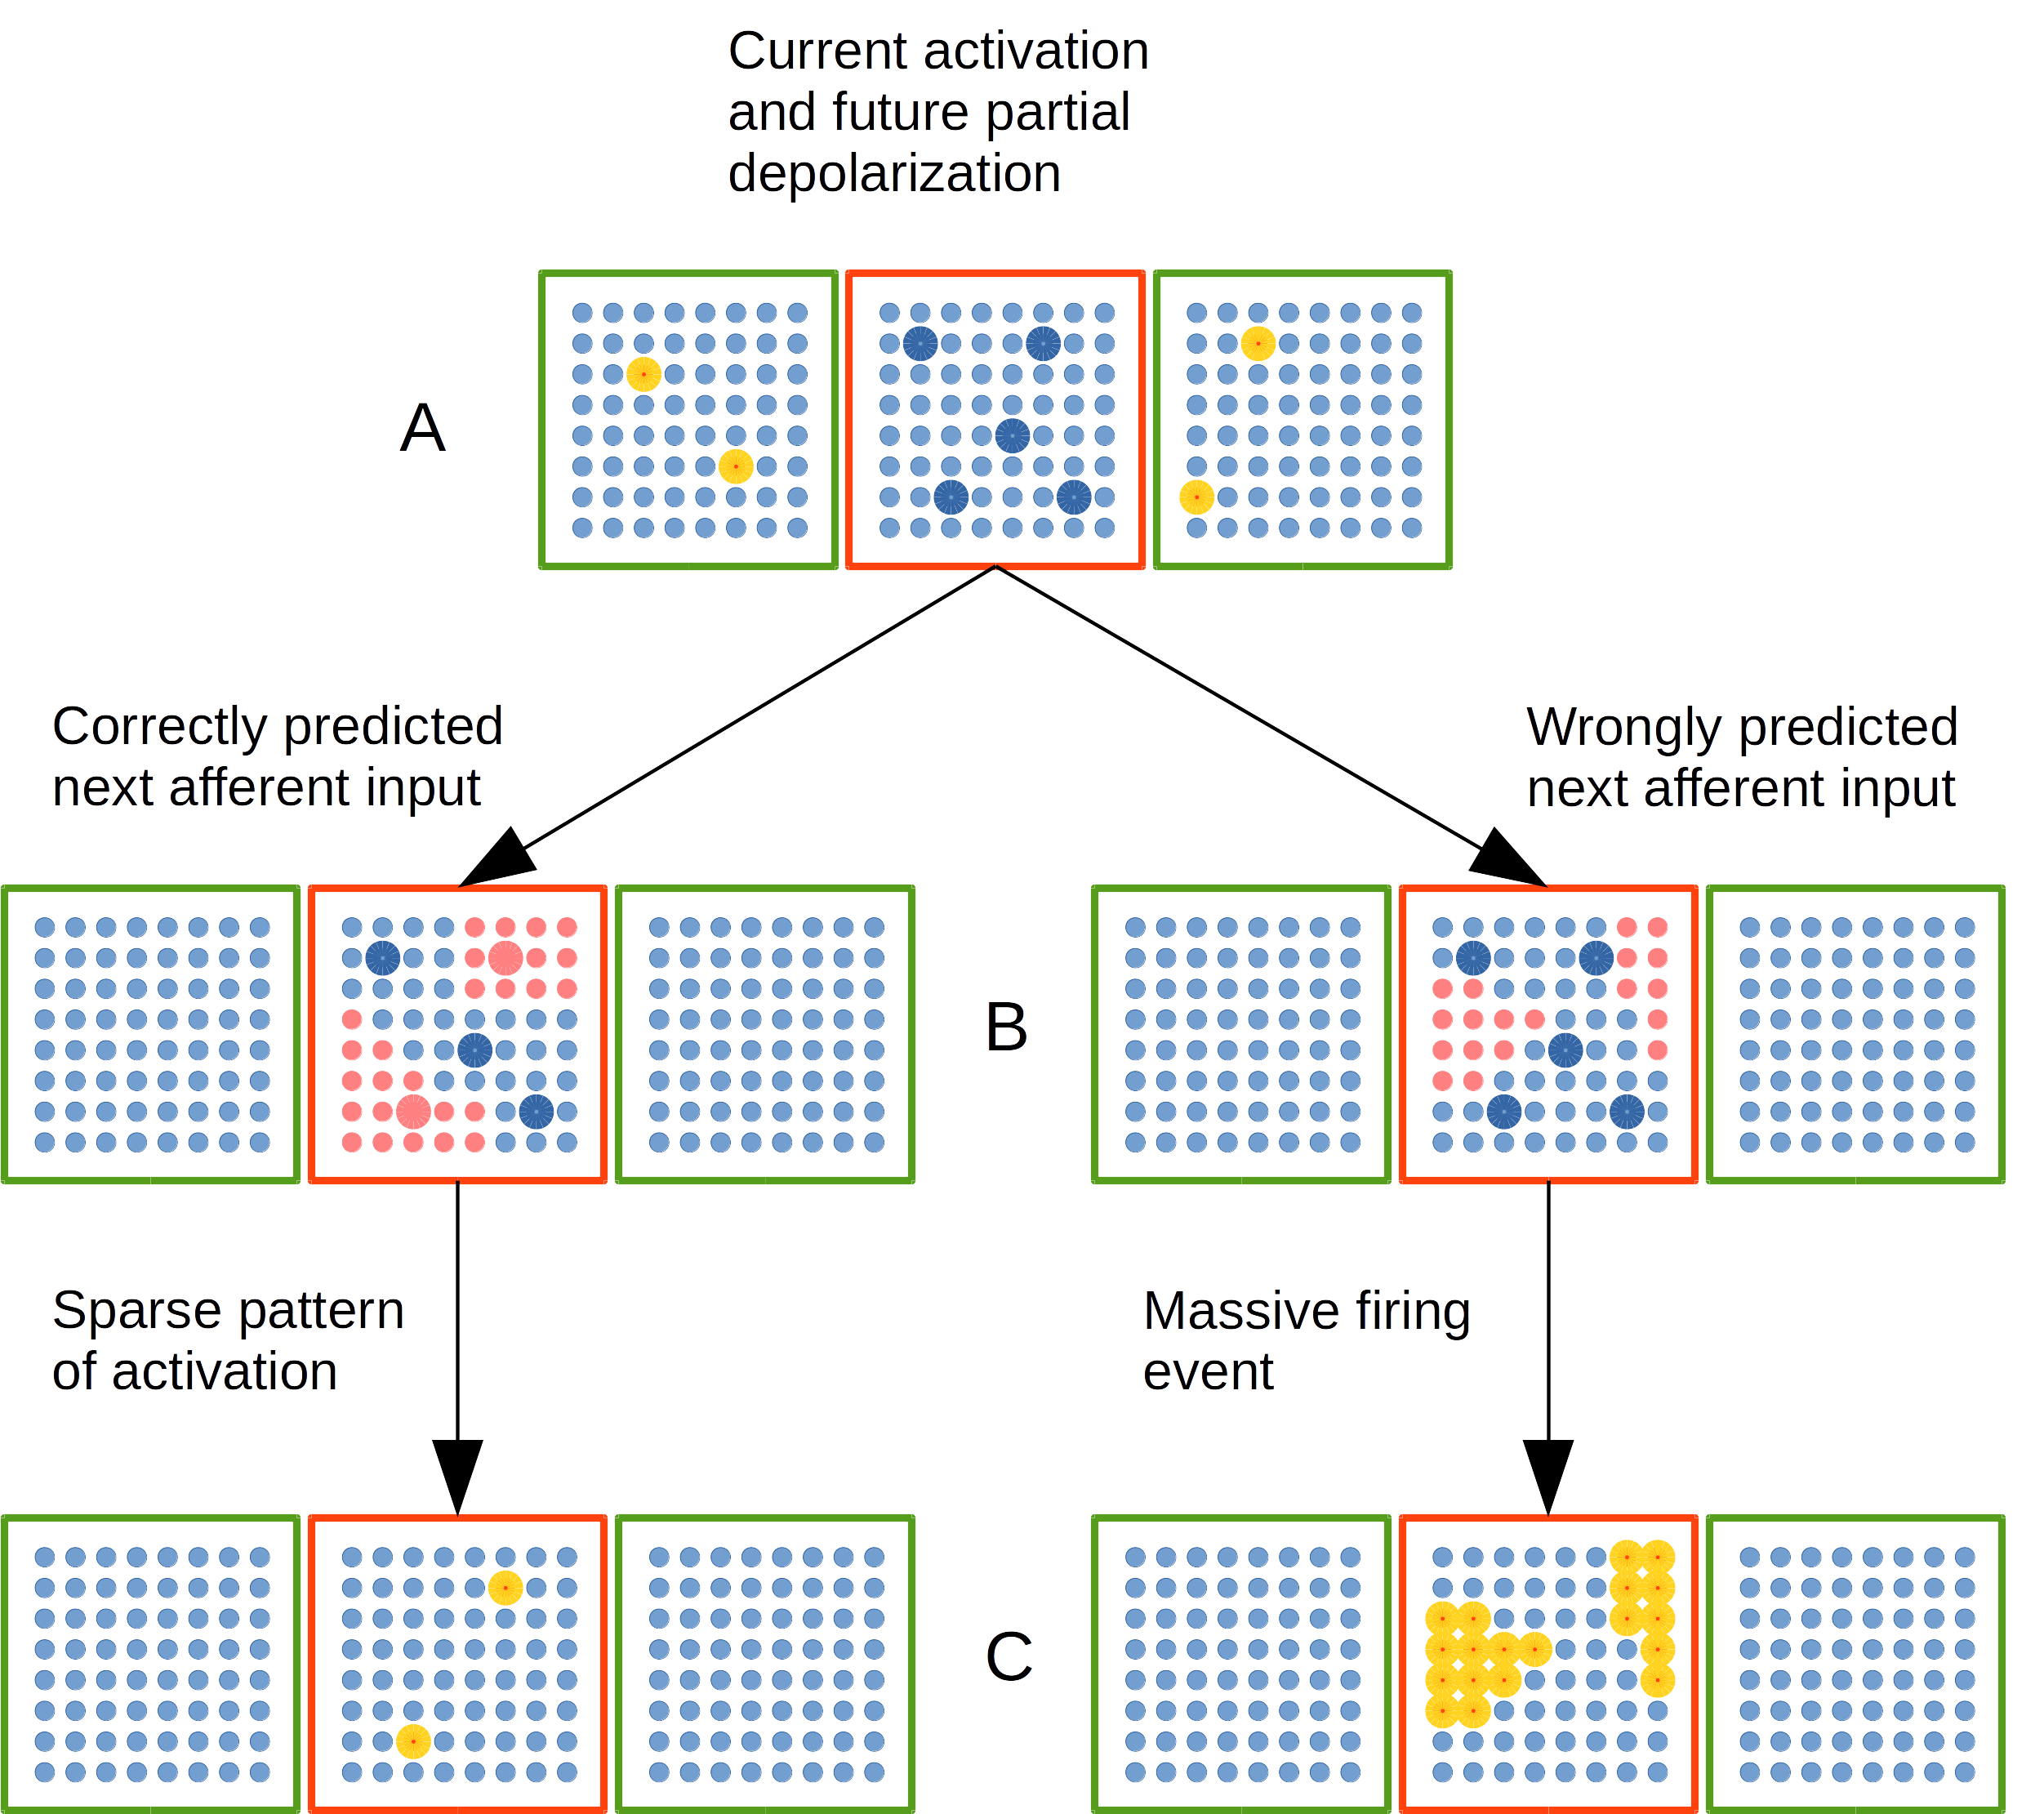
\includegraphics[width=0.7\textwidth]{Activation.png}
    \caption{Dynamic cellular activation in a \gls{cc} in the \gls{el}.
    A red cortical column is linked with two green cortical columns by means of distal dendrites.
    (A) Cellular activation in green \glspl{cc}--highlighted yellow cells--puts neural units
    in red \gls{cc} in a partially depolarized--predictive state highlighted in blue.
    (B) Cluster of neural cells activated by afferent inputs.
    Left: A substantial amount of partially depolarized cells are in the afferently excited cellular clusters.
    Right: There is no substantial amount of partially depolarized cells inside afferently excited cellular clusters.
    (C) \gls{cc} with active cellular units highlighted in yellow.
    Left: Sparse pattern of cellular activation.
    Right: Massive pattern of activation.}
    \label{fig:Activation}
\end{figure}

\pagebreak

Partial depolarization states put cell units in a predictive state generated by
the activations produced in the \gls{el} in previous time steps.
That is, lateral and apical activation in previous time steps constitutes a context in which
current afferent inputs are received.

From the group of units that tend to be depolarized by current afferent inputs from the \gls{mrstsa},
only a reduced sub-set of those units are likely to fire in the previous contextual firing history
in the \gls{el}--Fig. \ref{fig:Activation} C left.

In case there is no context, that is, none of the units which tend to be depolarized by afferent inputs
is partially depolarized by previous--lateral and apical--activations--Fig. \ref{fig:Activation} B right--,
all units in the afferent excited clusters will be active, covering more hypotheses for next inputs--Fig. \ref{fig:Activation} C right.

Each neural unit in a \gls{cc} establishes its state of partial depolarization based on the contribution from
distal dendritic branches from lateral and apical connections.
A dendritic branch will contribute to the partial depolarization of the soma in such cell only if such
dendritic branch exceeds an activation threshold by means of the contribution from its individual synapses
in the context of the patterns of activation in the previous time step.

This mechanism has compelling sequential properties \cite{hawkins_2016},
which have already been applied in the classification of artificially generated sequential data \cite{cui_2016}.
We apply such mechanism in the \gls{dsom} algorithm by adding the contribution of synapses--in a dendritic branch--
whose connections are linked with cells that were active in the previous time step in the \gls{el}.

















\subsection*{\glsfirst{mrstsa}}
\label{sec-mrstsa}

%In Chi T. et al. \cite{chi_2005}, a computational model of auditory analysis is described.
Chi T. et al. \cite{chi_2005} describe a computational model of auditory analysis.
The model is inspired by psychoacoustical and
neurophysiological findings in early and central stages of the auditory system.
Such model 
%provided
provides
an unified multiresolution representation of the spectral and temporal features
%which were 
which are
interpreted as critical for the perception of sound.

The original algorithm has a subcortical and a cortical stage.
For the subcortical stage, first an affine wavelet transform of the acoustic signal
represents the spectral analysis performed by the cochlear filter bank.
Second, the cochlear filter outputs are transduced into auditory-nerve
patterns by a hair cell stage consisting of a high-pass filter,
a nonlinear compression and a membrane leakage low-pass filter.
Third, a first-order derivative with respect to the tonotopic axis
followed by a half-wave rectifier
simulates the action of a lateral inhibitory
network postulated to exist in the cochlear nucleus,
which effectively enhances the frequency
selectivity of the cochlear filter bank.
The final output of this stage is obtained by integrating
over a short window, with time constant of 8 ms, mimicking
the further loss of phase locking observed
in the midbrain.

The cortical stage mimics aspects of the responses of higher
central auditory stages, especially \gls{a1}.
Functionally, this stage estimates the
spectral and temporal modulation content of the auditory
spectrogram. It does so computationally via a bank of filters
that are selective to different spectrotemporal modulation parameters
that range from slow to fast rates temporally, and
from narrow to broad scales spectrally. The \glspl{strf}
of these filters are also centered at
different frequencies along the tonotopic axis.

Since we prompt a parsimonious incorporation of neurophysiological
properties--mainly centered in cortical features--
we followed the main guidelines in the implementation of the cortical section of such model.

~\todo{weird sentence}

We implemented the initial stage in our model with the application of \gls{fft} to the audio vector
with a different sample window for each resolution.
We then extracted the power spectral density from each resolution.
In this way we obtained a multiresolution spectral analysis of the audio signal,
with high spectral and low temporal resolution for wider sample windows and
vice versa.
Such different time windows in the \gls{fft},
incorporated--at the same time--leakage low-pass filters with a time constant for each
resolution accounting for decrease of phase-locking in the auditory nerve.
We then applied a \gls{mfb} with 128 elements to each spectrum
in order to represent the spectral analysis performed by the cochlear filter bank.
Then, we convolved each resolution obtained in the last step along its tonotopic axis
with a complex multiresolution function whose real part
was a symmetric Mexican hat function and its imaginary part was its antisymmetric Hilbert transform.
With this strategy we incorporated the phenomena of symmetry \cite{shamma_1993}, bandwidth \cite{schreiner_1990}
and frequency modulation selectivity \cite{shamma_1993,heil_1992,mendelson_1985}
found in \gls{a1} and incorporated in the original algorithms \cite{wang_1995}.

We obtained the magnitude of each convolution and applied normalization to each time window
as a mean of automatic gain control in order to prioritize the information delivered by the
spectral configuration and not the absolute values delivered by the filters. 

By means of this constraint we account for the mechanical and chemical properties of hair cells in the mammalian inner ear
which constitute a transduction mechanism that appears to adapt to recent stimulus history in a way that can affect its gain
\cite{eatock_2000,holt_2000,le_goff_2005}. 
We decided to be conservative, not including
sound intensity dimension but just the shape of the filter responses.














\section*{Materials and methods}
\subsection*{Corpora generation}
\label{CorpGen}


We generate a corpora of 500 words with mono, di and trisyllabic randomly chosen English words with vocabularies of five words
using \gls{festival} Speech Synthesis \cite{festival2014}.

\begin{itemize}
	\item Monosyllabic vocabulary: \textit{map, dog, mouse, with, truck.} % and \textit{truck}.
	\item Disyllabic vocabulary: \textit{answer, doctor, teacher, summer, tennis.}  %and \textit{tennis}.
	\item Trisyllabic vocabulary: \textit{computer, telephone, rectangle, tomato, magazine.} % and \textit{magazine}.
\end{itemize}

%\todo[inline]{Silvio: can not see how these 15 words generate 500 words. Either I am missing something obvious or we need additional explanations}

We generate a cross synthesizer standard mark up language file with SABLE \cite{sable}.
In this file, we instruct \gls{festival} to generate a corpus with 500 words from a vocabulary of
5 words uttered by 10 different voices (8 males and 2 females) available from the synthesizer.

The organization of the corpus has certain rules and restrictions in order to avoid biases in the training processes.
The voices are sequentially chosen (pseudo-randomly) with the restriction that no voice could utter a second time until all the voices had uttered in their turns. Every voice utters two words per turn--in pseudo-random order--and no word is not be repeated until all the words are used by such voice. 

We use the following English speaking voices provided by Festival: \texttt{cmu\_us\_fem\_cg, cmu\_us\_gka\_cg, cmu\_us\_ksp\_cg, cmu\_us\_rxr\_cg, cmu\_us\_jmk\_cg, cmu\_us\_rms\_cg, cmu\_us\_slt\_cg, cmu\_us\_jmk\_arctic\_clunits, cmu\_us\_rms\_arctic\_clunits, cmu\_us\_slt\_arctic\_clunits}.

Every word in the audio file is followed by a silence gap whose time is equivalent to the uttering time of the monosyllabic word \textit{cat}, uttered by the same voice used for the last word. We use the \texttt{text2wave} program provided by Festival in order to generate a \texttt{wav} file from the SABLE file.

\subsection*{\glsfirst{mrstsa} Implementation}

We apply \gls{fft} to the audio files with a sample period of 8 milliseconds.
We use the FFTW package \cite{FFTW05, fftw}
with time windows of 8, 16, 32, 64 and 128 milliseconds in order to obtain
a multiresolution power spectral analysis of the signal.
%We then applied 
In addition, we apply the Mel Filter-Bank technique with 128 filters to each
spectral resolution and convolve such filters along their tonotopic axis.
For the convolution, we use a multiresolution complex function whose real part
is a Mexican hat function and its imaginary part is the corresponding Mexican hat Hilbert transformation.
%-Fig. \ref{fig:Multi}.

%\begin{figure}[h!]
    %\centering
    %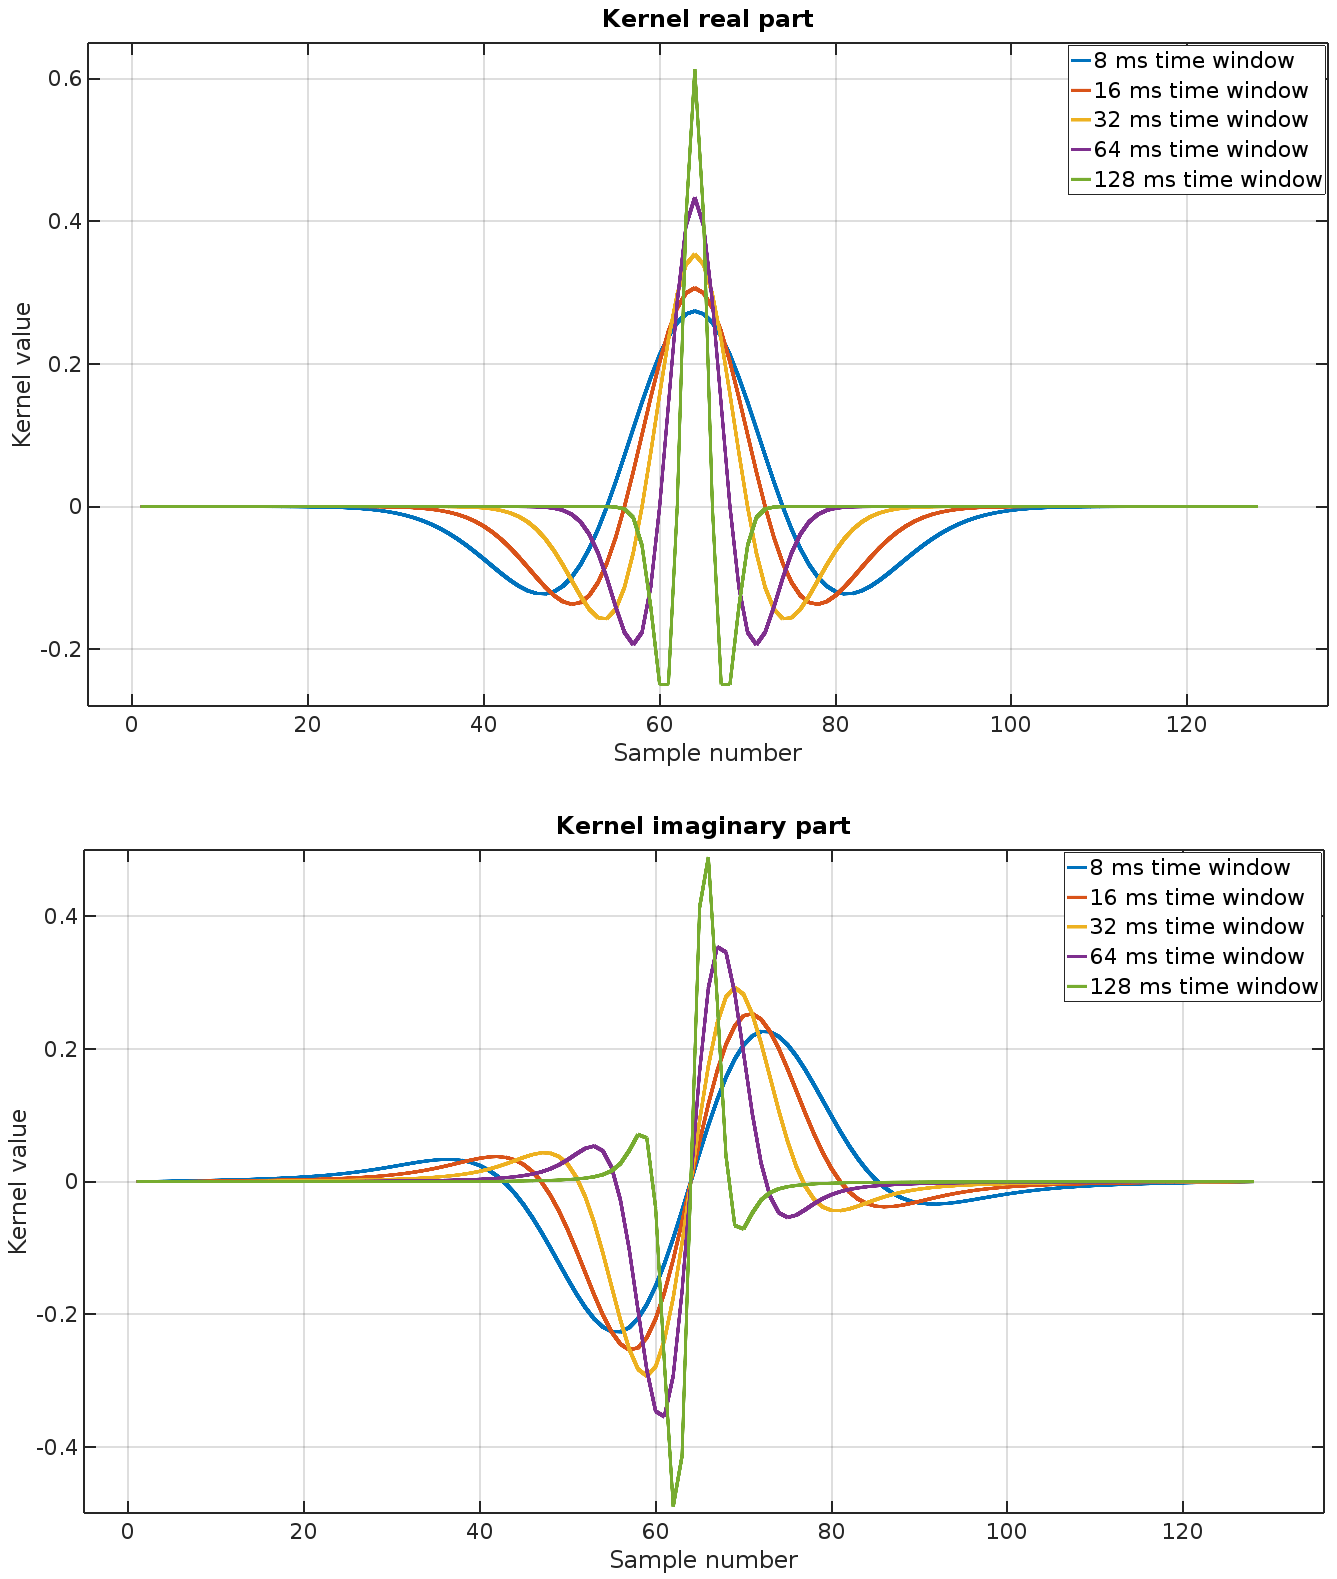
\includegraphics[width=0.7\textwidth]{Multi.png}
    %\caption{Multiresolution complex kernels. Such kernels are convolved with Mel Filter Bank outputs along their tonotopic axis.
	    %Each kernel has a different coefficient
    %and is convolved with its corresponding power spectral resolution.
    %The function coefficients are 10 for 8 ms time window, 8 for 16 ms time window, 6 for 32 ms time window, 4 for 64 ms time window
    %and 2 for 128 ms time window.}
    %\label{fig:Multi}
%\end{figure}

The function coefficients are 10 for the 8 ms time window, 8 for the 16 ms time window, 6 for the 32 ms time window, 4 for the 64 ms time window
and 2 for the 128 ms time window. We then compute the magnitude from the convolution and normalize in each time step.
By means of this procedure we obtain from the audio file a multiresolution spectro-temporal response composed by
an array of 128 columns--one column per filter--and 5 rows--one row per resolution--with real numbers which range from
0 to 1, for each time step.









\subsection*{\glsfirst{el} Implementation}
\label{ELImp}

We implement an \gls{el} with 225 \glspl{csom} arranged in a two-dimensional
array of 15 by 15 \glspl{cc}. Each \gls{cc} is automatically distributed using individual locations along its afferent inputs in a uniform way.
Each \gls{cc} receives afferent information by means of
two-dimensional afferent receptive fields of 5 by 227 filters centered at individual locations over the \gls{mrstsa}.
We enable the wraparound property in order to make each receptive field span the entire
\gls{mrstsa} array.
We also instruct each column to receive only 31 inputs, which is a minor percentage of such
receptive field.
Individual afferent inputs for each \gls{cc} are chosen randomly in the \gls{el} initialization. 

For this model instance we implement only distal lateral dendritic branches since there are
no more \glspl{cl} from which to bring information through apical dendritic branches.
We configure each \gls{cc} to have a lateral receptive field with 9 by 9 neighboring \glspl{cc}
and to receive information from 72 of the 81 \glspl{cc} in the receptive field--a 90\% of the receptive field.

Each \gls{cc} is composed of a two-dimensional array with 15 by 15 (225) neural units and
each unit in a column could be potentially connected with only 6 neural units from each linked neighboring column. 
That is, each neural unit in a \gls{cc} ends up with 72 lateral dendritic branches with 6 potential connections each
(432 distal potential synapses per cellular unit).
Such potential synapses are randomly chosen for each neural cell and for each dendritic branch in the cell during the Encoder initialization procedure.
The \gls{el} consists of 50625 cellular units with 1569375 proximal synapses and 21870000 distal synapses.

We train the \gls{el} using a 500 word corpora generated by the procedure described in section \nameref{CorpGen}.
The training procedure consists of 4 stages and for each stage the \gls{el} receives the same corpus 4 times.

During each learning stage, certain parameters--such as the learning rates in proximal and distal synapses and the lateral
intra-column interaction--are exponentially and progressively decreased from an initial value, which also decreases
for each successive stage.
An additional stage is executed with the learning parameters fixed.

The sparsity in the activation for each \gls{cc} is 99\% (just 2 neural units out of 225 could be active for normal activation events).
On the other hand, the afferent excitation affects 10\% of the units inside the clusters in each \gls{cc}
(22 neural units, which could be activated in case of a \gls{mfe}; Fig. \ref{fig:Activation}).









\subsection*{\glsfirst{svm} Classification}
\label{Classif}

%% For figure citations, please use "Fig" instead of "Figure".
%Nulla mi mi, Fig~\ref{fig1} venenatis sed ipsum varius, volutpat euismod diam. Proin rutrum vel massa non gravida. Quisque tempor sem et dignissim rutrum. Lorem ipsum dolor sit amet, consectetur adipiscing elit. Morbi at justo vitae nulla elementum commodo eu id massa. In vitae diam ac augue semper tincidunt eu ut eros. Fusce fringilla erat porttitor lectus cursus, \nameref{S1_Video} vel sagittis arcu lobortis. Aliquam in enim semper, aliquam massa id, cursus neque. Praesent faucibus semper libero.

%% Place figure captions after the first paragraph in which they are cited.
%\begin{figure}[!h]
%\caption{{\bf Bold the figure title.}
%Figure caption text here, please use this space for the figure panel descriptions instead of using subfigure commands. A: Lorem ipsum dolor sit amet. B: Consectetur adipiscing elit.}
%\label{fig1}
%\end{figure}

We use supervision by means of the \gls{svm} classification
method, receiving the outputs from each algorithm \cite{CC01a, libsvm}. We do this to test the invariance properties in the phonetic features abstracted by the \gls{el} in comparison
with the phonetic features abstracted by the \gls{mrstsa}, 
(Fig. \ref{fig:Experiment}).

We use the silent temporal gaps between consecutive words in the \gls{mrstsa} outputs in order to introduce marks to
detect the beginning and end of each word.

We then produce a vector per word in the corpus summing the activity in the \gls{mrstsa} as well as in the \gls{el} between consecutive marks
and use such vectors to train both classifiers (the one receiving outputs from the \gls{mrstsa} and the one receiving outputs from the \gls{el}).

Afterwards, we scale the vectors--as the \gls{libsvm} documentation suggests--
so as to improve the classification performance.
We train and test the \gls{svm} classifiers using 5-fold cross-validation
and configure them to use a linear kernel with one parameter $C$ which
we swept to find the best trained model for each classifier.












\subsection*{Computational Setup}
\label{Comp_setup}

We implement our algorithms in standard
\CC14 using the \gls{oop} paradigm in a set of classes interrelated by inheritance and composition.
We implement proximal afferent and distal inter-columnar connectivity  
as well as minimum-maximum margins in afferent synaptic weights in the \glsfirst{el} class.
We configure such class as a composition of objects of class \glsfirst{csom}.
The main member in the \gls{el} class is a \gls{stl} vector of \gls{csom} objects.
A complete diagram of the hierarchical inheritance and compositional structure of the implementation
can be seen in Fig. \ref{fig:Skeleton}.

\begin{figure}[h!]
    \centering
    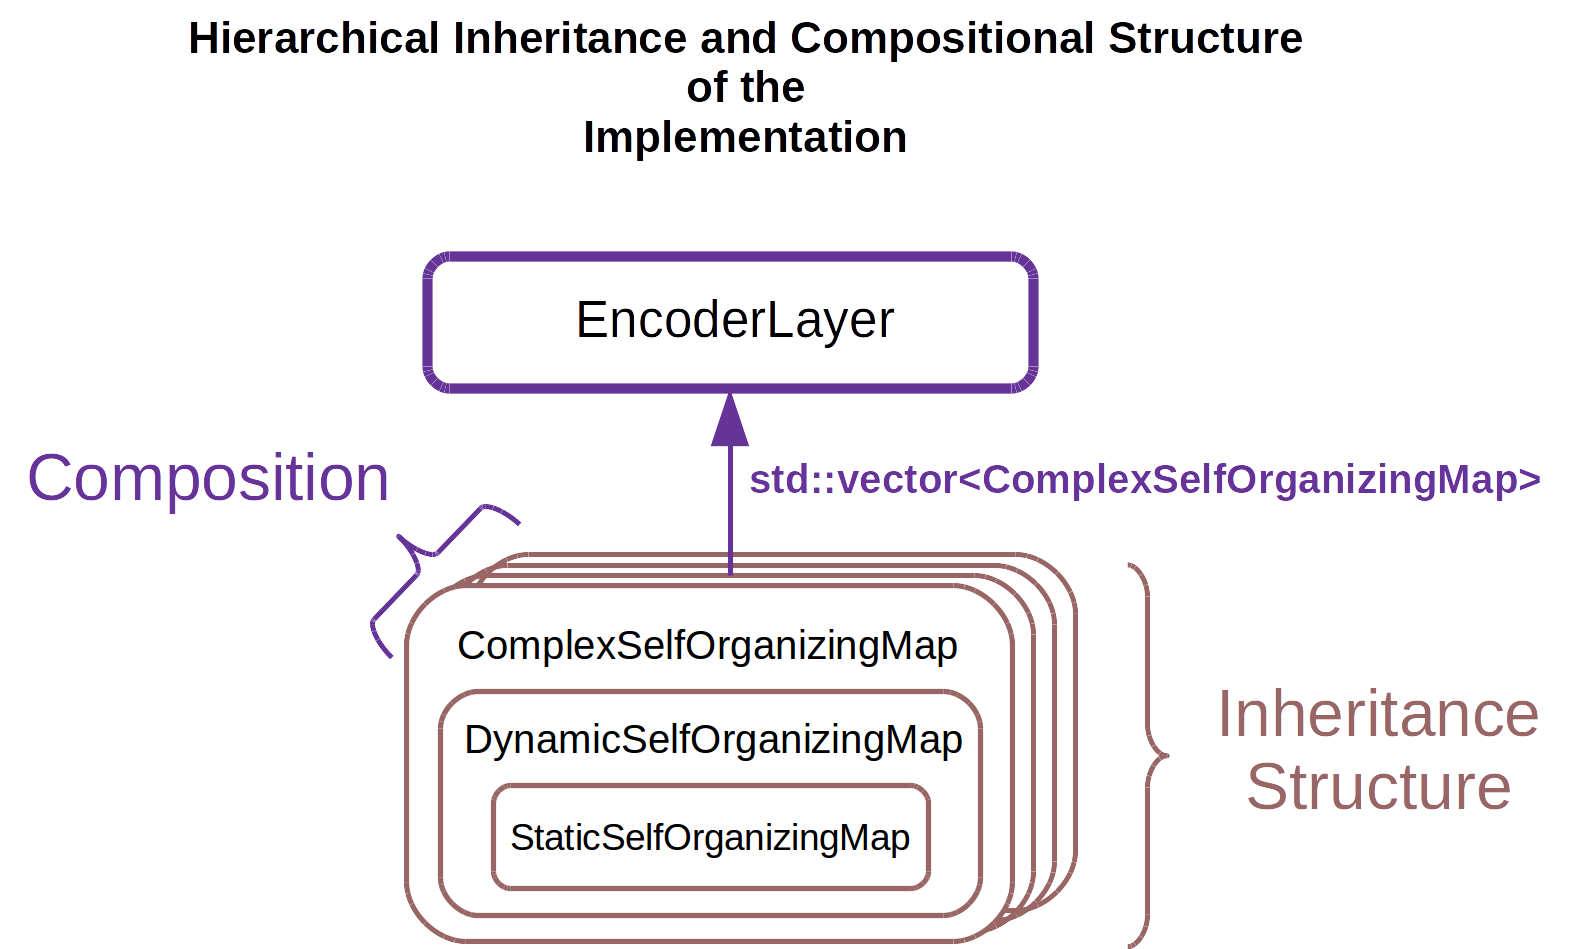
\includegraphics[width=0.8\textwidth]{Skeleton.png}
    \caption{Hierarchical Inheritance and Compositional Structure of the Model Implementation.
    \glsfirst{csom} inherits from \glsfirst{dsom} which inherits from \glsfirst{ssom}.
    The \glsfirst{el} is formed by the composition of a set of \glspl{csom} gathered
    in a std::vector \glsfirst{stl} container.}
    \label{fig:Skeleton}
\end{figure}

\pagebreak

We parallelize the \gls{el} class by means of a hybrid \gls{mpi}+\gls{omp} paradigm.
We distribute \glspl{csom} among \gls{mpi} ranks as a deck of cards is distributed among different players.
Each \gls{mpi} rank ends up with one or more \glspl{csom} and the \glspl{csom} in each rank are distributed
among different \gls{omp} threads (Fig. \ref{fig:EncoderParallelization} A and B respectively).
Information among \gls{mpi} ranks must be transferred in each time step.
We gather all the information corresponding to the \glspl{csom}
in each rank and then use \gls{mpi} Bcast function to transmit such information
using a special comunication protocol by means of which we specify the boundaries
in the information corresponding to each \gls{csom}(Fig. \ref{fig:EncoderParallelization} C).
By means of this strategy each MPI rank has to call \gls{mpi} Bcast just once
in order to transmit its data.
The \gls{el} uses \gls{mpi} I/O parallel file system to save its status in Matlab/Octave format
(Fig. \ref{fig:EncoderParallelization} D).
Each \gls{mpi} rank gathers all the data corresponding to its \glspl{csom} in the \gls{el} and
communicates the part of the file it will use to the other \gls{mpi} ranks, in order to store the data
without interfering with the other ranks in the \gls{mpi} environment.
Then, each \gls{mpi} rank saves all its data with a unique call to \gls{mpi} Write. 


\begin{figure}[h!]
    \centering
    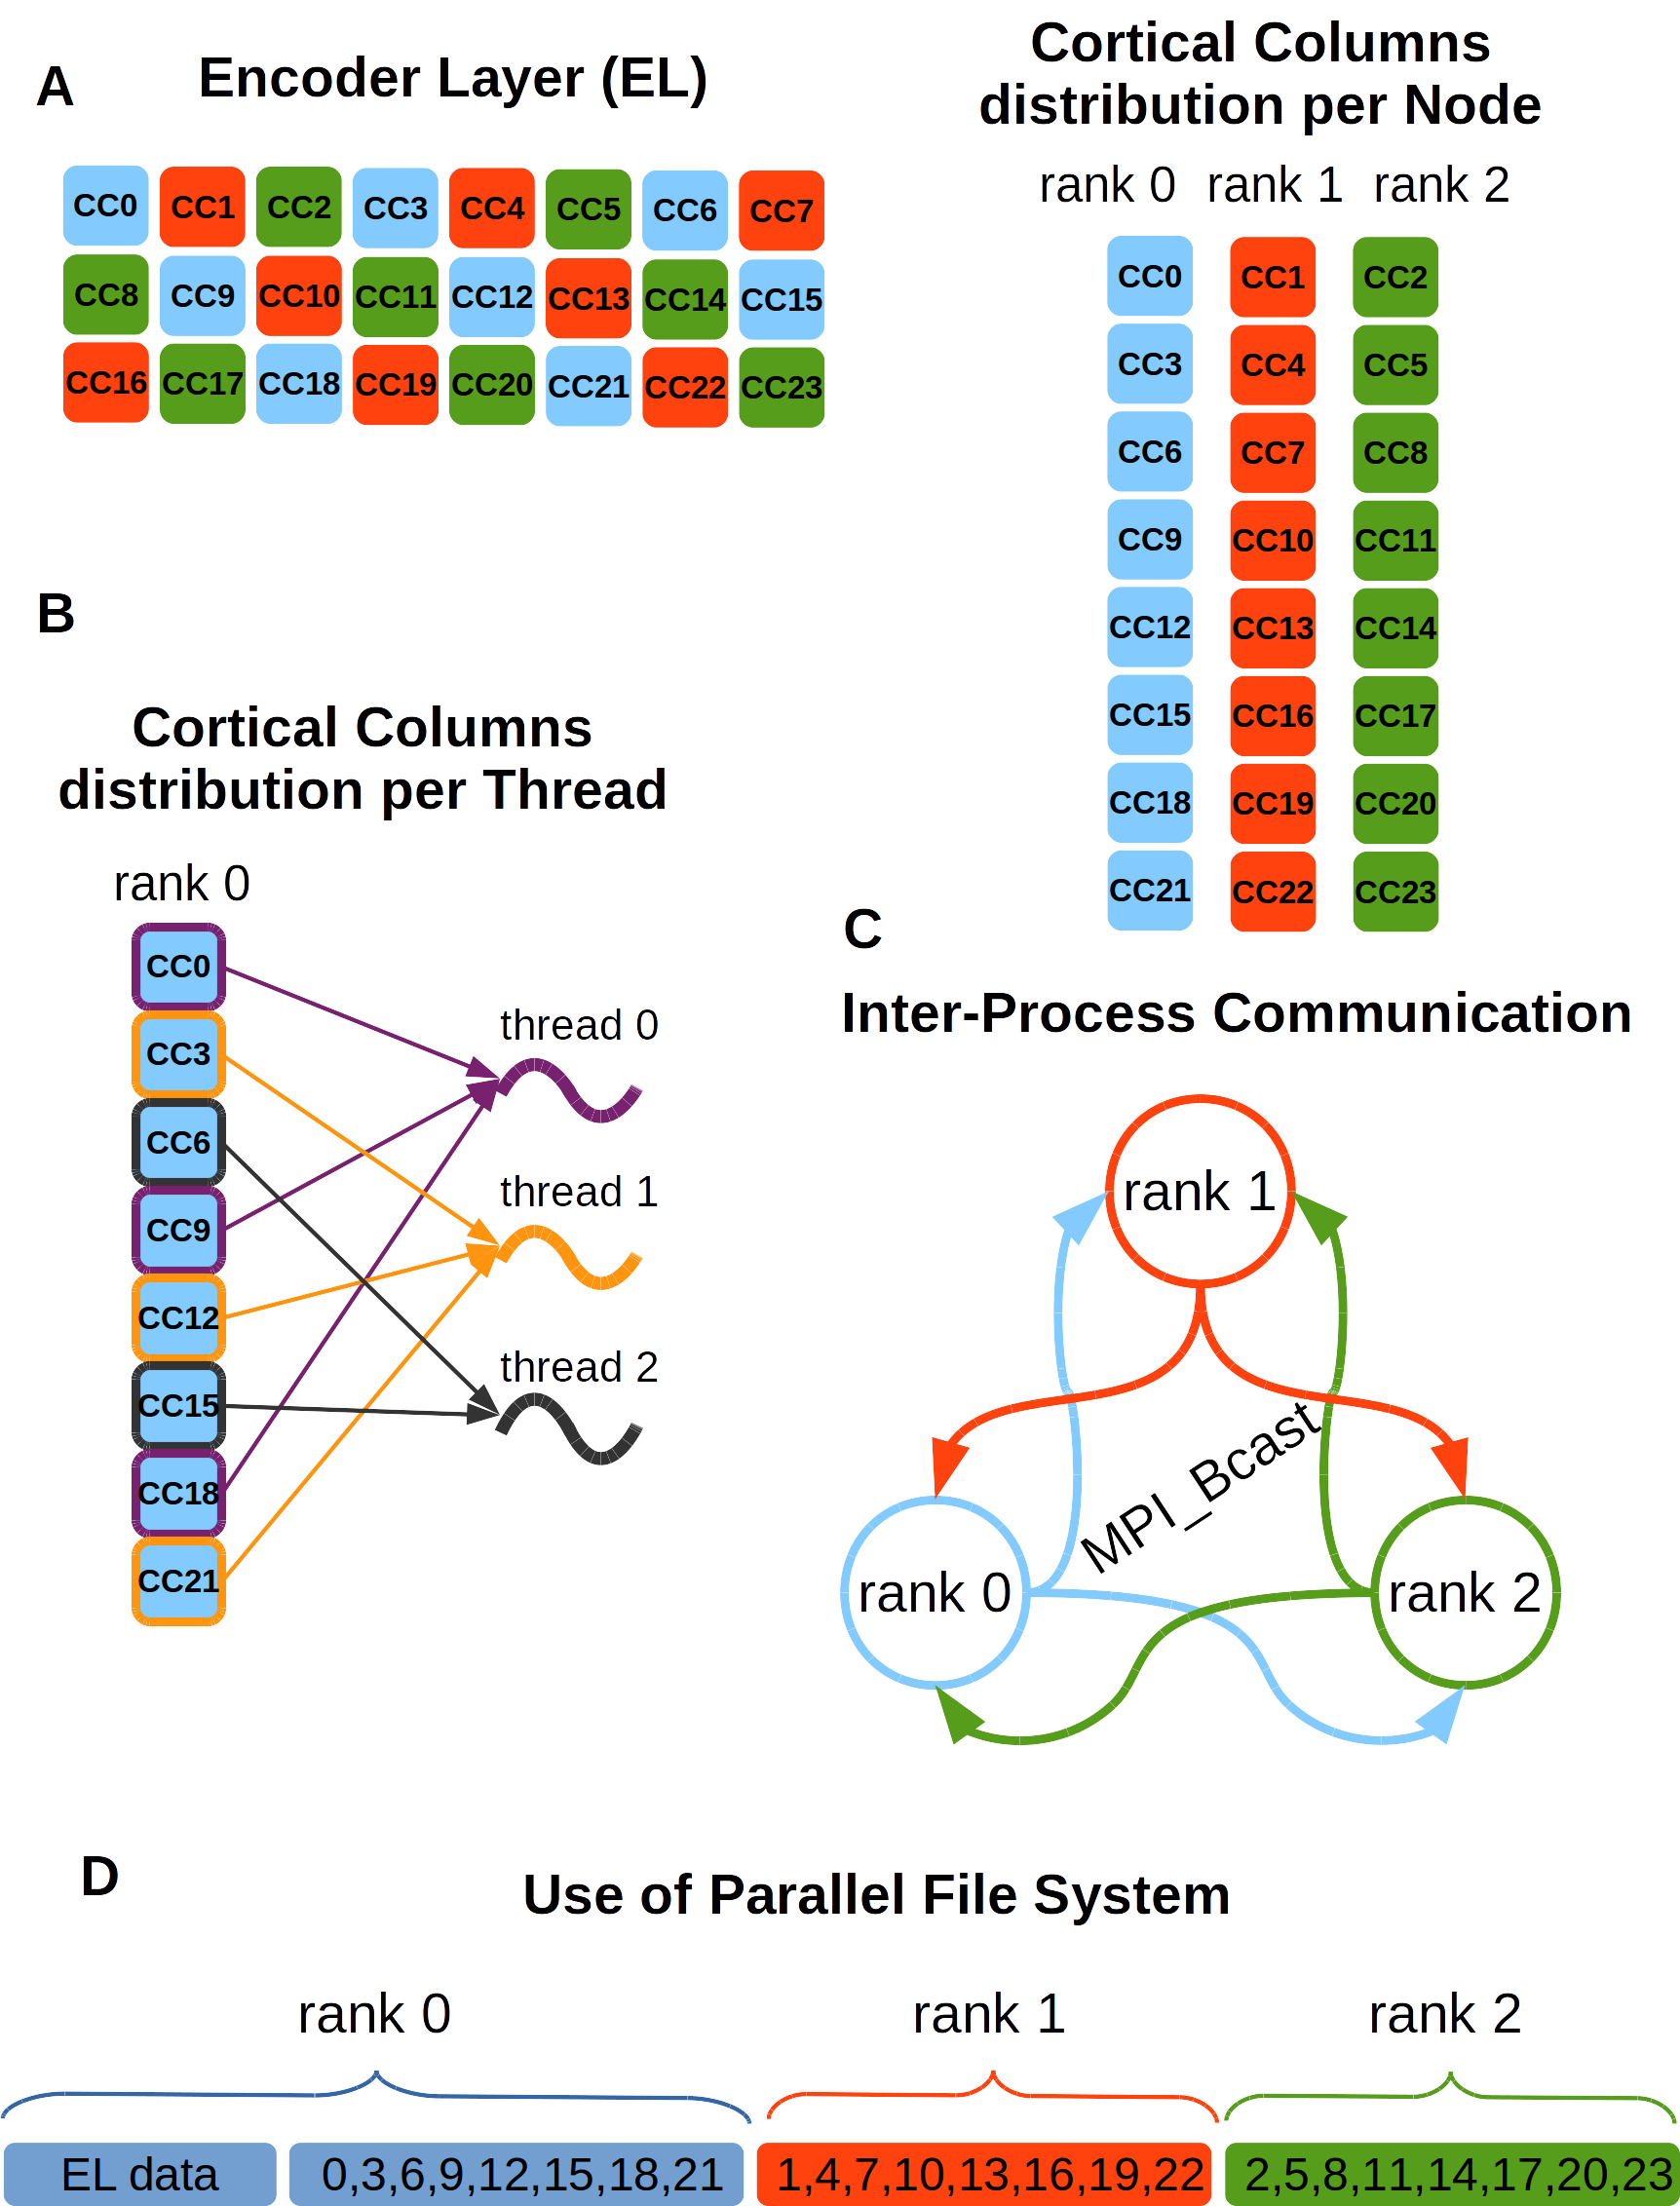
\includegraphics[width=0.7\textwidth]{EncoderParallelization.png}
    \caption{\glsfirst{el} \gls{mpi}+\gls{omp} parallelization. (A) Distribution of \gls{csom} objects in an \gls{el} with
    3 by 8 (24) \glspl{cc} among three \gls{mpi} ranks with three \gls{omp} threads per rank.
    Certain ranks could take care of a different number of
    \glspl{csom} depending on the number of \gls{mpi} ranks as well as the number of \glspl{cc} in the \gls{el}.
    (B) Each \gls{mpi} rank distributes its \glspl{csom} among different threads in the same fashion.
    (C) \gls{mpi} \gls{ipc} among different ranks. \gls{ipc} is carried out at each time step since each \gls{mpi} rank 
    requires the complete \gls{el} output at each time step.
    Each \gls{mpi} rank broadcasts the information corresponding to its \glspl{cc} to the other ranks in the \gls{mpi}
    environment.
    (D) \gls{el} information distribution in a file to save its status.
    Each \gls{mpi} rank puts the formated data corresponding to its \glspl{csom} in a \gls{stl} stringstream class template.
    Rank 0 also takes care of the \gls{el} structure, connectivity and parameters.
    Once each rank has its stringstream with the formated data, it communicates its file view to the other ranks.
    Then each rank writes its stream of bytes in parallel without interfering with other ranks in the \gls{mpi} environment.
    An \gls{el} with a different number of ranks can load the same file without affecting the final results.
    Each rank in the new \gls{el} loads the complete file in a \gls{stl} stringstream class template and then takes the
    informations that concern it from such structure.}
    \label{fig:EncoderParallelization}
\end{figure}

\pagebreak

The implementation has Checkpoint and Restart capacity in its training stage where there is total flexibility
in terms of the number of ranks with which the execution is restarted. A cortical layer could have been saved
with $n$ ranks and such layer could be restarted with $m$ ranks without affecting the final results.


It is important to mention that the number of \glspl{cc} shown in
Fig. \ref{fig:EncoderParallelization} is merely illustrative and
does not reflect the real numbers in terms of computational resources used for this implementation.

%The simulations performed for this work were carried out in an \gls{alcf}
%Allocation at \gls{anl}.
%We run the algorithms on Cooley Cluster with simulations using 25 nodes 
%(9 \glspl{cc} per node and one node per \gls{mpi} rank)
%and 8 threads per node/rank (almost one thread per \gls{cc}).

We performed all computational experiments on Cooley, a visualization and analysis cluster at Argonne National Laboratory. We ran the simulations using 25 nodes (9 \glspl{cc} per node and one node per \gls{mpi} rank) and 8 OpenMP threads per node/rank (almost one thread per \gls{cc}).




% Results and Discussion can be combined.
\section*{Results}
%Nulla mi mi, venenatis sed ipsum varius, Table~\ref{table1} volutpat euismod diam. Proin rutrum vel massa non gravida. Quisque tempor sem et dignissim rutrum. Lorem ipsum dolor sit amet, consectetur adipiscing elit. Morbi at justo vitae nulla elementum commodo eu id massa. In vitae diam ac augue semper tincidunt eu ut eros. Fusce fringilla erat porttitor lectus cursus, vel sagittis arcu lobortis. Aliquam in enim semper, aliquam massa id, cursus neque. Praesent faucibus semper libero.

%% Place tables after the first paragraph in which they are cited.
%\begin{table}[!ht]
%\begin{adjustwidth}{-2.25in}{0in} % Comment out/remove adjustwidth environment if table fits in text column.
%\centering
%\caption{
%{\bf Table caption Nulla mi mi, venenatis sed ipsum varius, volutpat euismod diam.}}
%\begin{tabular}{|l+l|l|l|l|l|l|l|}
%\hline
%\multicolumn{4}{|l|}{\bf Heading1} & \multicolumn{4}{|l|}{\bf Heading2}\\ \thickhline
%$cell1 row1$ & cell2 row 1 & cell3 row 1 & cell4 row 1 & cell5 row 1 & cell6 row 1 & cell7 row 1 & cell8 row 1\\ \hline
%$cell1 row2$ & cell2 row 2 & cell3 row 2 & cell4 row 2 & cell5 row 2 & cell6 row 2 & cell7 row 2 & cell8 row 2\\ \hline
%$cell1 row3$ & cell2 row 3 & cell3 row 3 & cell4 row 3 & cell5 row 3 & cell6 row 3 & cell7 row 3 & cell8 row 3\\ \hline
%\end{tabular}
%\begin{flushleft} Table notes Phasellus venenatis, tortor nec vestibulum mattis, massa tortor interdum felis, nec pellentesque metus tortor nec nisl. Ut ornare mauris tellus, vel dapibus arcu suscipit sed.
%\end{flushleft}
%\label{table1}
%\end{adjustwidth}
%\end{table}


%%PLOS does not support heading levels beyond the 3rd (no 4th level headings).
%\subsection*{\lorem\ and \ipsum\ nunc blandit a tortor}
%\subsubsection*{3rd level heading} 
%Maecenas convallis mauris sit amet sem ultrices gravida. Etiam eget sapien nibh. Sed ac ipsum eget enim egestas ullamcorper nec euismod ligula. Curabitur fringilla pulvinar lectus consectetur pellentesque. Quisque augue sem, tincidunt sit amet feugiat eget, ullamcorper sed velit. Sed non aliquet felis. Lorem ipsum dolor sit amet, consectetur adipiscing elit. Mauris commodo justo ac dui pretium imperdiet. Sed suscipit iaculis mi at feugiat. 

%\begin{enumerate}
	%\item{react}
	%\item{diffuse free particles}
	%\item{increment time by dt and go to 1}
%\end{enumerate}


In this paper, we study the level of invariance in the phonetic features abstracted by the \gls{el},
by means of comparing such representations with the multiresolution spectro-temporal auditory features
returned by the \gls{mrstsa} algorithm.

To this end, we evaluate the features returned by each algorithm in different word classification tasks.
In order to asses the word classification performance in each algorithm, we use \gls{svm}
technique--section \nameref{Classif}--with 
the experimental setup depicted in Fig. \ref{fig:Experiment}.

In the experimental procedure we first train the \gls{el}--section \nameref{ELImp}--with a corpus generated by the method described in section \nameref{CorpGen}.
Afterwards, we process the same corpus with the \gls{el} in inference mode.
In such mode, the \gls{el} processes the information with its learning properties disabled.
In this manner, during inference, the \gls{el} does not modify its synapses and just returns patterns of activation in
response to the stimuli it receives.
We then use the outputs from the \gls{mrstsa} and the \gls{el} in inference mode to train the
\gls{svm} classifiers with the procedure depicted in section \nameref{Classif}.
The cross validation training performances are shown in Table~\ref{SVM_Training}.

\begin{table}[h!]
\centering
\caption{\gls{svm} 5-fold cross validation training results}
\begin{tabular}{|l|l|l|}
\hline
                   & MRSTSA & Encoder Layer \\ \hline
Monosyllabic Words & 98.8\% & 99\%          \\ \hline
Disyllabic Words   & 98\%   & 97.8\%        \\ \hline
Trisyllabic Words  & 97.6\% & 98\%          \\ \hline
\end{tabular}
\label{SVM_Training}
\end{table}

\pagebreak

In a second stage, we run the \gls{el} in inference mode again, but this time we affect the original corpus by means of different kind of variances. 
We test the performances of the--already trained--classifiers in the presence of the features returned by the algorithms in response to the corpus affected
by the variances which we introduce to original corpora by means of Audacity \cite{audacity}.
The variances introduced to the original corpus include white noise, reverberation and pitch variations.
The classification performances are shown in Figs. \ref{fig:MONO_ACC}, \ref{fig:DI_ACC} and \ref{fig:TRI_ACC}.

\begin{figure}[h!]
    \centering
    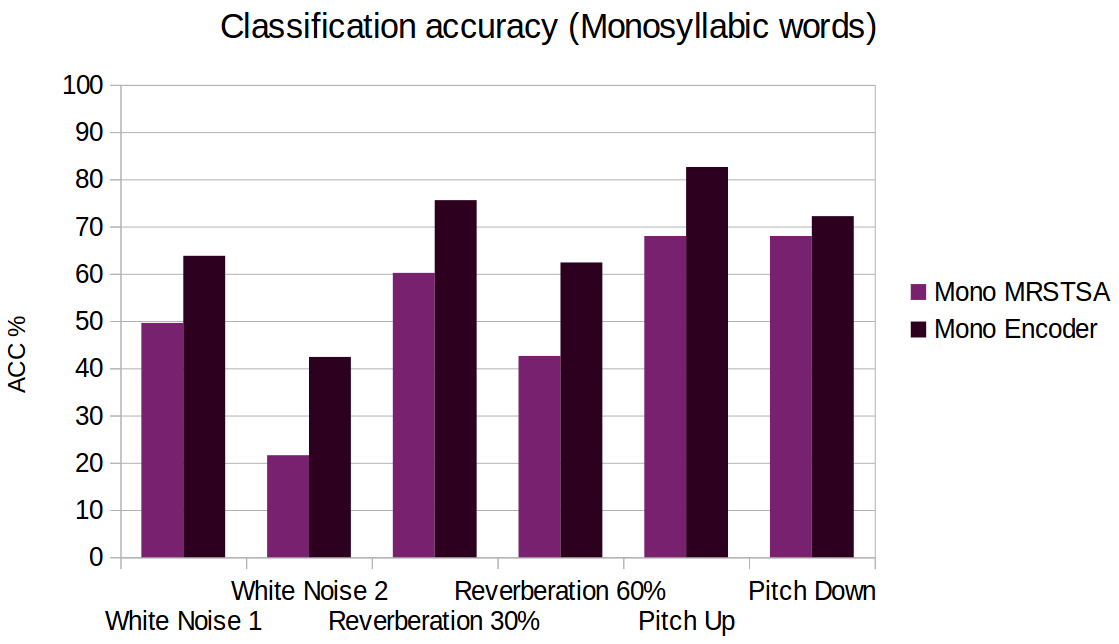
\includegraphics[width=0.9\textwidth]{MONO_ACC.png}
    \caption{\gls{mrstsa} and \gls{el} classification accuracies against different variances introduced to the original signals
    for \textbf{monosyllabic words}.
    White Noise 1 determines a \gls{snr} average \gls{rms} power rate of 19.8 dB while White Noise 2 13.8 dB.
    Reverberation 30\% determines a \gls{rt} value of 0.61 seconds while Reverberation 60\% determines a \gls{rt} value of 1.78 seconds.
    Pitch Up determines a pitch move from E to G, while Pitch Down determines a pitch move from E to C.}
    \label{fig:MONO_ACC}
\end{figure}

\begin{figure}[h!]
    \centering
    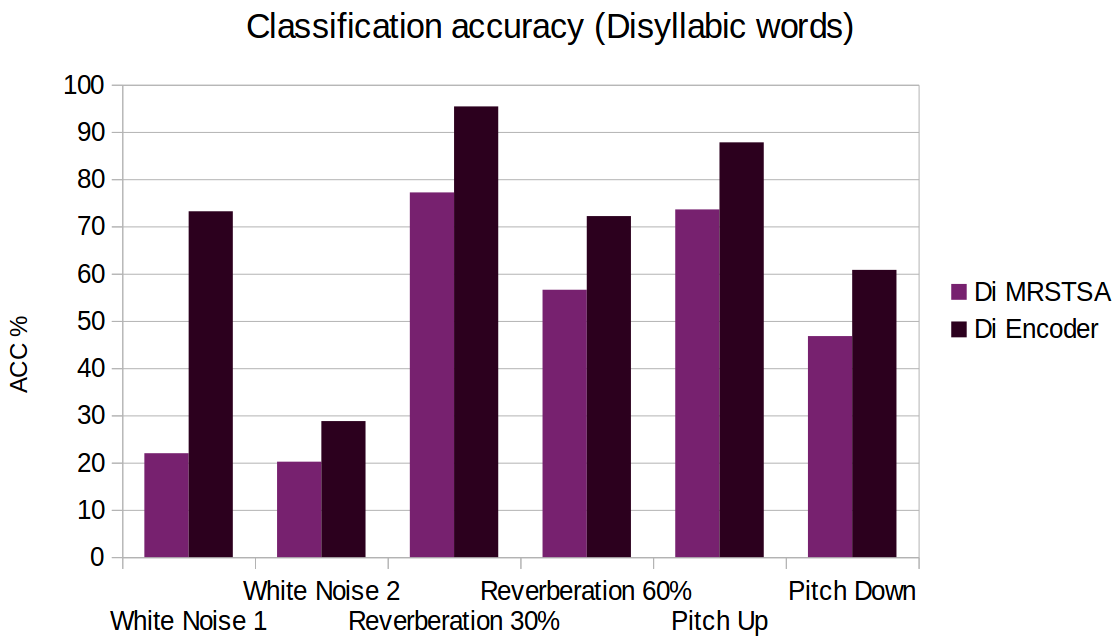
\includegraphics[width=0.9\textwidth]{DI_ACC.png}
    \caption{\gls{mrstsa} and \gls{el} classification accuracies against different variances introduced to the original signals
    for \textbf{disyllabic words}.
    White Noise 1 determines a \gls{snr} average \gls{rms} power rate of 19.8 dB while White Noise 2 13.8 dB.
    Reverberation 30\% determines a \gls{rt} value of 0.61 seconds while Reverberation 60\% determines a \gls{rt} value of 1.78 seconds.
    Pitch Up determines a pitch move from E to G, while Pitch Down determines a pitch move from E to C.}
    \label{fig:DI_ACC}
\end{figure}

\begin{figure}[h!]
    \centering
    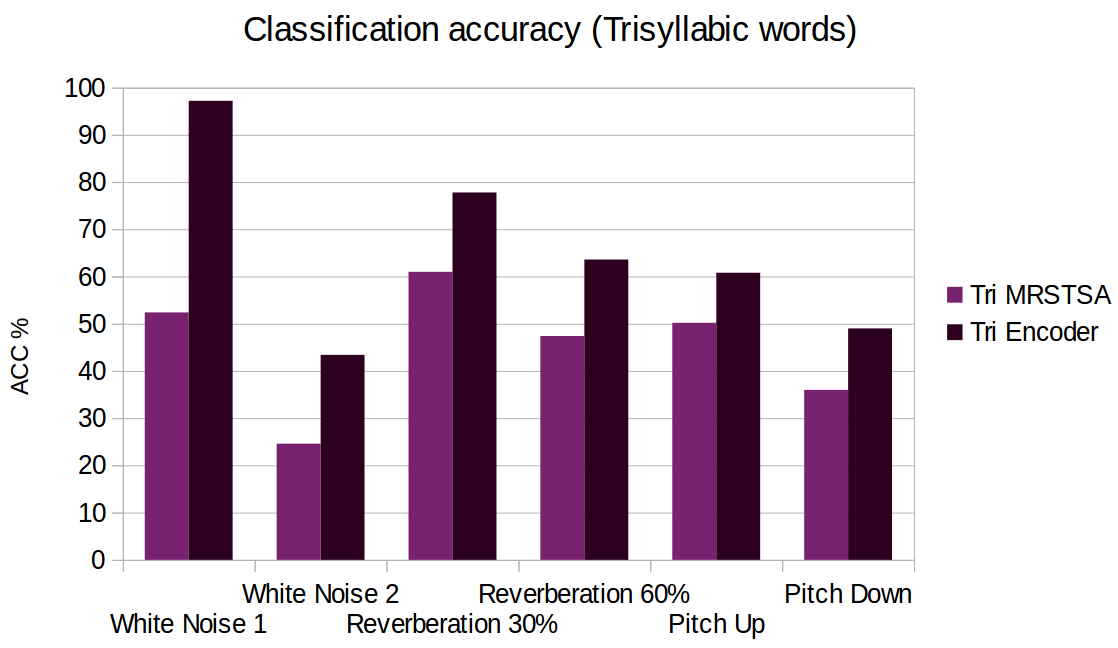
\includegraphics[width=0.9\textwidth]{TRI_ACC.png}
    \caption{\gls{mrstsa} and \gls{el} classification accuracies against different variances introduced to the original signals
    for \textbf{trisyllabic words}.
    White Noise 1 determines a \gls{snr} average \gls{rms} power rate of 19.8 dB while White Noise 2 13.8 dB.
    Reverberation 30\% determines a \gls{rt} value of 0.61 seconds while Reverberation 60\% determines a \gls{rt} value of 1.78 seconds.
    Pitch Up determines a pitch move from E to G, while Pitch Down determines a pitch move from E to C.}
    \label{fig:TRI_ACC}
\end{figure}

\pagebreak

Referring to white noise, we introduce additive white noise to the original signal with a signal-noise average \gls{rms} power
rate of 19.9 dB (White Noise 1) and 13.8 dB (White Noise 2).
In terms of reverberation, we modify the original signal by means of \gls{rt} values of 0.61 seconds (Reverberation 30\%)
and 1.78 seconds (Reverberation 60\%).
\gls{rt} Is the time that a signal takes to decrease its amplitude to 60 dBs under its initial value.
In reference to pitch variations, we modify the signal pitch in +20\% (from E to G) (Pitch Up) and in--20\% (from E to C) (Pitch Down).

\iffalse
\begin{figure}[h!]
    \centering
    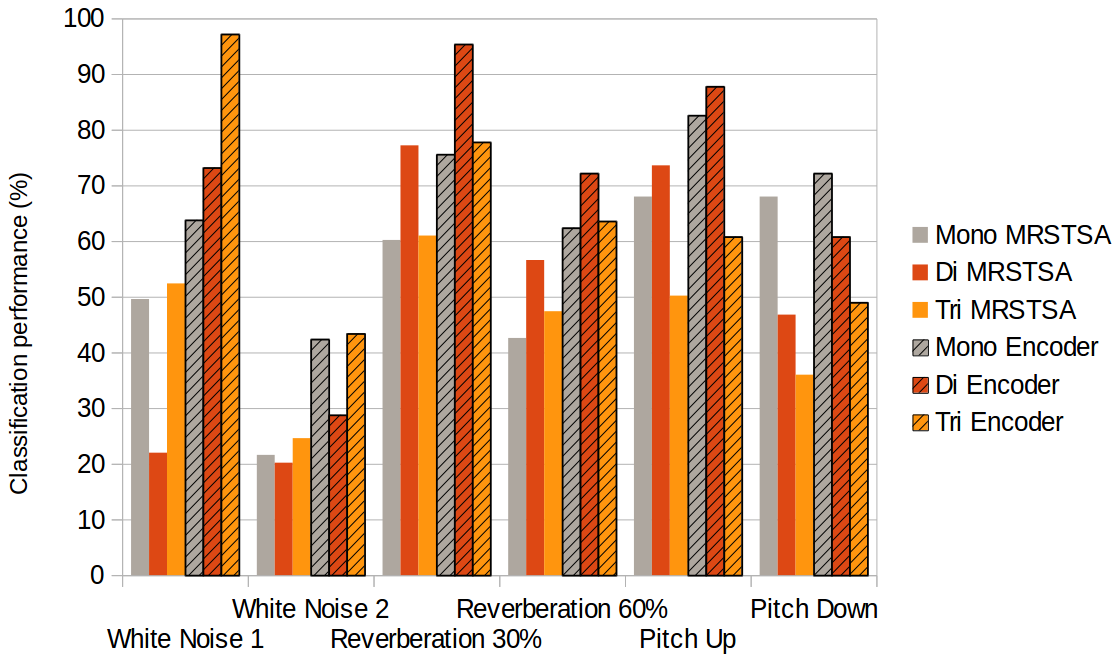
\includegraphics[width=0.9\textwidth]{Classification.png}
    \caption{\gls{mrstsa} and \gls{el} classification performances against different variances introduced to the original signals.
    Mono means monosyllabic words, Di means disyllabic words and Tri means trisyllabic words.
    White Noise 1 determines a \gls{snr} average \gls{rms} power rate of 19.8 dB while White Noise 2 13.8 dB.
    Reverberation 30\% determines a \gls{rt} value of 0.61 seconds while Reverberation 60\% determines a \gls{rt} values of 1.78 seconds.
    Pitch Up determines a pitch move from E to G, while Pitch Down determines a pitch move from E to C.}
    \label{fig:Classification}
\end{figure}
\fi


In Figs. \ref{fig:MONO_ACC}, \ref{fig:DI_ACC} and \ref{fig:TRI_ACC}
we report a 5 way word classification accuracy for mono, di and trisyllabic word corpora affected by
white noise, reverberation and pitch variations.
As can be seen in the figures, the \gls{el} outperforms the \gls{mrstsa} in all cases.
Such behavior persists for multisyllabic words.

\iffalse
Beyond that, information about the improvement rate of the \gls{el} with respect to the \gls{mrstsa} algorithm in relation to the
length of the words could shed light on the
cortical predictive mechanisms performance in the \gls{el}.
In Fig. \ref{fig:Improvement} we show the classification performance improvements achieved by the \gls{el} in relation to the \gls{mrstsa} algorithm.


\begin{figure}[h!]
    \centering
    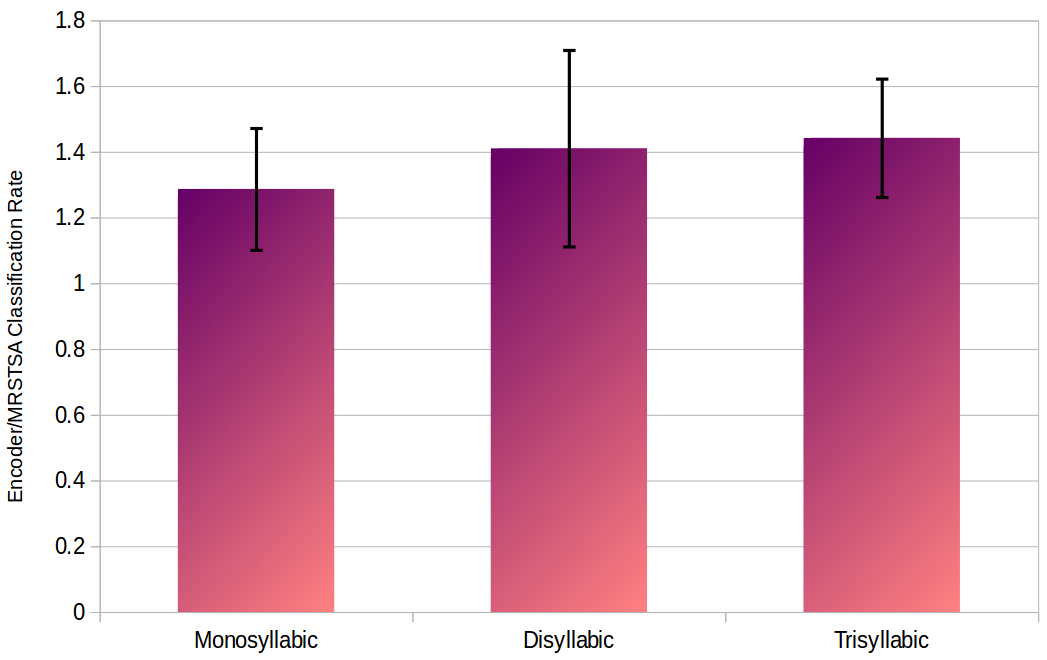
\includegraphics[width=0.7\textwidth]{Improvement.png}
    \caption{Encoder/MRSTSA Classification Performance Rate.
    The improvement, provided by the \gls{el} over the \gls{mrstsa}, in word classification performance grows with the number of syllables in the words.
    Quotients are computed between average performances along variances.
    Error bars correspond to the average of all possible quotient combinations between average performances affected by their \glspl{se}
    {\tiny $\abs*{\left (\frac{Encoder~Performance~Average ~\pm~ Encoder~Standard~Error}{MRSTSA~Performance~Average ~\pm~ MRSTSA~Standard~Error}\right )-Average~Performance~Quotient}$}}.
    \label{fig:Improvement}
\end{figure}

We measure the improvements achieved by the \gls{el} over the \gls{mrstsa} on the average performances across variances
for mono, di and trisyllabic words.
In such figure, it can be seen a trend which shows an increment in the classification improvement for words
with more syllables for the vocabularies used in this research.
Such trend is more meaningful for the jump from one to two syllables than for the jump from two to three syllables.
\fi


Fig. \ref{fig:AV_ACC} shows average classification accuracies across all variances for mono, di and trisyllabic words.
As can be seen in the figure, according to \textbf{Standard Error} bars, the encoder layer clearly shows
a sustained superiority across words with different number of syllables.
 

\begin{figure}[h!]
    \centering
    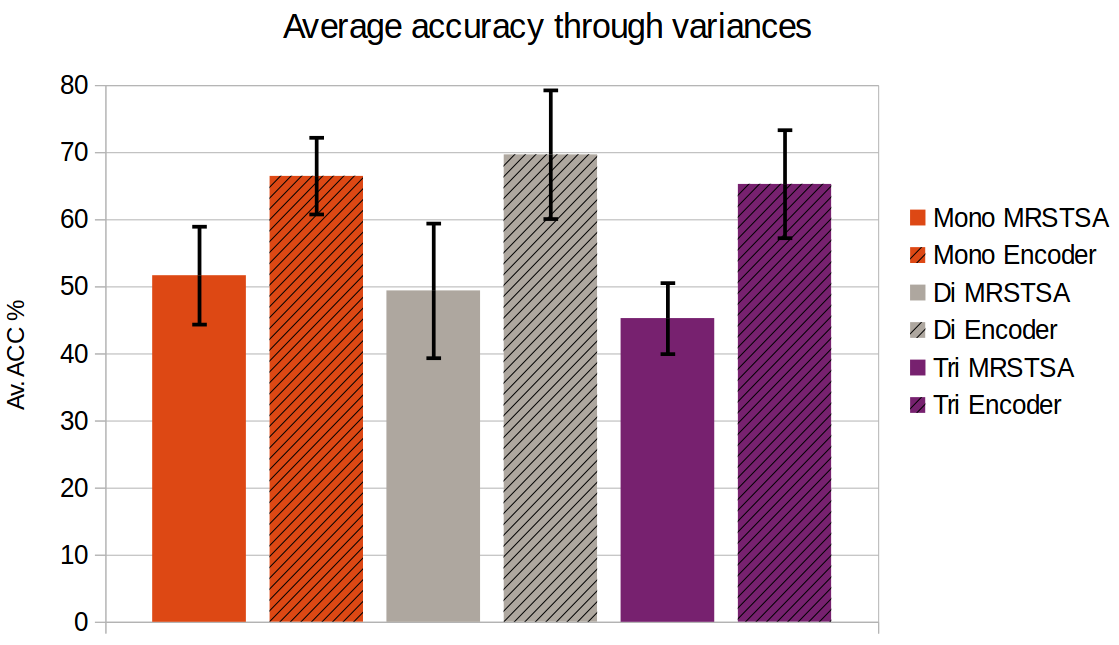
\includegraphics[width=0.9\textwidth]{AV_ACC.png}
    \caption{Average classification accuracies across all variances for mono, di and trisyllabic words with Standard Error bars.
    Mono means monosyllabic words, Di means disyllabic words and Tri means trisyllabic words.}
    \label{fig:AV_ACC}
\end{figure}






%\subsection*{Sed ac quam id nisi malesuada congue}

%Nulla mi mi, venenatis sed ipsum varius, volutpat euismod diam. Proin rutrum vel massa non gravida. Quisque tempor sem et dignissim rutrum. Lorem ipsum dolor sit amet, consectetur adipiscing elit. Morbi at justo vitae nulla elementum commodo eu id massa. In vitae diam ac augue semper tincidunt eu ut eros. Fusce fringilla erat porttitor lectus cursus, vel sagittis arcu lobortis. Aliquam in enim semper, aliquam massa id, cursus neque. Praesent faucibus semper libero.

%\begin{itemize}
	%\item First bulleted item.
	%\item Second bulleted item.
	%\item Third bulleted item.
%\end{itemize}

\section*{Discussion}

%Nulla mi mi, venenatis sed ipsum varius, Table~\ref{table1} volutpat euismod diam. Proin rutrum vel massa non gravida. Quisque tempor sem et dignissim rutrum. Lorem ipsum dolor sit amet, consectetur adipiscing elit. Morbi at justo vitae nulla elementum commodo eu id massa. In vitae diam ac augue semper tincidunt eu ut eros. Fusce fringilla erat porttitor lectus cursus, vel sagittis arcu lobortis. Aliquam in enim semper, aliquam massa id, cursus neque. Praesent faucibus semper libero~\cite{bib3}.

Results from our experiments support the hypothesis that certain anatomical and neurophysiological features--mainly in cortical tissue--could be crucial for auditory perceptual phonetic invariance.
% GKT This is the beginning of sentence
%The cortical columnar organization with afferent raw micro-columnar activation, in combination with fine tunedpartial depolarization by distal \gls{nmda} lateral dendritic active elements--with \glspl{mfe} in front of prediction faults and \glspl{sdr} in front of lateral inhibition--plusthe dynamic plasticity provided by \gls{stdp} mechanisms showed to be relevant in order to acquire the phonotactic rules immersed in the vocabularies. 
% GKT this is the end
%~\todo{The sentence above is too long. Can not change it easily without altering its meaning}
These features have already been explained in terms of their properties
%and potential~
\cite{hawkins_2016},
but more
%precisely
specifically
in terms of their sequence learning capabilities \cite{cui_2016}.
%To the best of our knowledge, our
Our work is among the first to model
%(successfully)
the neurophysiological features tested in word classification tasks. In our model,
%and implementation,
distal synapses make continuous individual contributions and our anatomical micro-columnar organization acquires its physiological behavior spontaneously from learning.
We have tested these features with hundreds of cortical columns, each combining several micro-columns with stochastic afferent activation, which requires considerable computational effort (see section \nameref{Comp_setup}).

%<<<<<<< HEAD
%Results from our experiments support the hypothesis that certain anatomical and neurophysiological features   
%-mainly in cortical tissue--could by crucial for auditory perceptual phonetic invariance.
%In the case of the research presented here, we report that cortical columnar organization with afferent raw micro-columnar activation, in combination
%with fine tuned
%partial depolarization by distal \gls{nmda}
%lateral dendritic active elements--with \glspl{mfe} in front of prediction faults and \glspl{sdr} in front of lateral inhibition--plus
%the dynamic plasticity provided by \gls{stdp} mechanisms showed to be relevant in order to acquire the phonotactic rules immersed in the vocabularies. 

%~\todo{The sentence above is too long. Can not change it easily without altering its meaning}


%An important part of such features have already been explained in terms of its properties and potential \cite{hawkins_2016},
%but more precisely in terms of its sequence learning capabilities \cite{cui_2016}.
%Yet, to the best of our knowledge there are no precedents of such neurophysiological features tested in word classification tasks as the ones carried out here.
%Beyond that, our approach presents substantial differences in terms of feature algorithmic implementation.
%In our implementation, distal synapses make continuous individual contributions and
%our anatomical micro-columnar organization acquires its physiological behavior spontaneously from learning.
%We also test such features in a realization with hundreds of cortical columns each combining several micro-columns with stochastic afferent activation which require
%considerable computational effort (see section \nameref{Comp_setup}).

%To understand how phonetic categories
%are acquired, several computational theories have been developed.
%In the context of such theories, the main idea has
%been to explain relevant aspects of phonetic acquisition neglecting details
%about how the brain might provide such
%computations \cite{rasanen_2012}.
%In contrast, the approach in this research is to gather
%potentially relevant biological aspects which could be
%significant in terms of information processing
%in the mammalian auditory cortex.

%A previous research on unsupervised feature learning for audio classification used \glspl{cdbn} \cite{Lee:2009:UFL:2984093.2984217}. 
%In such work it was tested the classification performance of a model with two layers in a 39 way phone classification accuracy task on
%the test data \gls{timit} for various numbers of training sentences.
%=======

Although other computational theories have been developed to explain relevant aspects of phonetic acquisition~\cite{rasanen_2012}, our approach is to gather potentially relevant biological aspects which could be significant in terms of information processing in the mammalian auditory cortex. Prior research on unsupervised feature learning for audio classification used \glspl{cdbn} \cite{Lee:2009:UFL:2984093.2984217}. 
In this work, the authors tested classification performance of a model with two layers in a 39-way phone classification accuracy task on the test data \gls{timit} for various numbers of training sentences.
The first layer never outperformed the \gls{mfcc} algorithm that was used as input for the network.
Furthermore, such work did not report the second layer performance since it could not outperform the first one.
The maximum performance reported for the first layer was 64.4\% vs. a performance of 79.6\% for the \gls{mfcc}.
It was just possible to report a performance of 80.3\% by means of combining both, the \gls{mfcc} and the first layer in the \gls{cdbn}.

In a more recent work, the capacity of \glspl{dmn}--a modification of \glspl{dnn} feed-forward architecture that uses a max-out activation function--to handle environmental noise was investigated into different broad phonetic classes and for different noise conditions \cite{silos_2016}.  In such experiments--with the exception of fricatives phonemes for 15 dB \gls{snr} Street Noise--accuracy never exceeded 70\%. Furthermore, performance was seriously impaired in the presence of 15 dB \gls{snr} white noise, resulting in classification accuracy  well below 60\% in all cases.

On the other hand, we reported classification performances of--for example--97.2\% on the \gls{el} vs. 52.4\% on the \gls{mrstsa} for trisyllabic words against 19.8 dB \gls{snr} white noise (Fig. \ref{fig:TRI_ACC}) and performances well above 40\% for mono and trisyllabic words against 13.8 dB \gls{snr} white noise (Figs. \ref{fig:MONO_ACC} and \ref{fig:TRI_ACC}). We also reported that the \gls{el} outperformed the \gls{mrstsa} for all the test conditions (Fig. \ref{fig:AV_ACC}) and that this behavior was sustained through different number of syllables in the words for the vocabularies used in this research (Fig. \ref{fig:AV_ACC}).

Although this is a compelling scenario, we have to be cautious since we cannot ignore important experimental differences among previous research results. First, the training material was very different in such works. We used corpora generated by synthesized voices instead of standardized \gls{timit} corpora.
Given the high quality of the voices synthesized by \gls{festival} \cite{festival2014} and its flexibility in order to compose different kind of corpora--even with words that does not exist in any language--we considered that this was an appropriate initial experimental procedure to test our approach. 
Second, we pursued multisyllabic words classification tasks in contrast to the phone classification experiments carried out in previous research
since we mainly aim to test the dynamic sequential capability of our model to acquire the phonotactic rules behind the training vocabularies. 
Finally, we reported results on 5-way classification tasks vs. performance on 39-way classification tasks in \cite{Lee:2009:UFL:2984093.2984217}. 
On the one hand, this last difference acts in favour of our approach considering that it is easier to classify one category among 5 than one among 39.
On the other hand, it is important to highlight that previous works have a more extended training material with more vocabularies, more speakers, etc.
In our case, we train our model with 500 words from a vocabulary of just 5 words uttered by 10 voices.
Those are undoubtedly more difficult training conditions for our approach. 

Our main objective was to assess the sequential phonetic invariance exhibited by the \gls{el} under strictly controlled experimental conditions in which we precisely knew the levels of noise, reverberation and pitch variations with which the stimulus was affected. In our work, the \gls{el} training material included just the original corpora with 500 words. The \gls{el} was never exposed--during learning--to the kind of disturbances used to test its classification performance. The experimental profile applied in this work (Fig. \ref{fig:Experiment}) makes it clear that the \gls{el} is completely unsupervised and that all supervision is limited to the \gls{svm} algorithm. This is an important result to demonstrate the biological plausibility of our implementation since phonotactic constraints in a human language are learned incidentally \cite{BRENT199693,saffran_1997} and therefore, no supervision could be supported under such behavioral circumstances.

%We know that more tests--in different scenarios--with different and standardized corpora (such as \gls{timit})
%will be needed to analyze the capacities of this approach more deeply. Nevertheless, we conclude that our neurocomputational model exhibits a significant level of phonetic generalization with the capacity to acquire phonotactic rules with a small sample size and to generalize to novel environmental contexts. 










\section*{Conclusion}

%CO\textsubscript{2} Maecenas convallis mauris sit amet sem ultrices gravida. Etiam eget sapien nibh. Sed ac ipsum eget enim egestas ullamcorper nec euismod ligula. Curabitur fringilla pulvinar lectus consectetur pellentesque. Quisque augue sem, tincidunt sit amet feugiat eget, ullamcorper sed velit. 

%Sed non aliquet felis. Lorem ipsum dolor sit amet, consectetur adipiscing elit. Mauris commodo justo ac dui pretium imperdiet. Sed suscipit iaculis mi at feugiat. Ut neque ipsum, luctus id lacus ut, laoreet scelerisque urna. Phasellus venenatis, tortor nec vestibulum mattis, massa tortor interdum felis, nec pellentesque metus tortor nec nisl. Ut ornare mauris tellus, vel dapibus arcu suscipit sed. Nam condimentum sem eget mollis euismod. Nullam dui urna, gravida venenatis dui et, tincidunt sodales ex. Nunc est dui, sodales sed mauris nec, auctor sagittis leo. Aliquam tincidunt, ex in facilisis elementum, libero lectus luctus est, non vulputate nisl augue at dolor. For more information, see \nameref{S1_Appendix}.


In this paper, we analyze the sequential phonotactic invariant representations of high levels auditory pathway responses to complex phonetic sound stimuli.  We research such representations in relation to potentially relevant features in the auditory cortex. We incorporate such features in a computational model--inside the \gls{el} stage of a model called \gls{cstm}--and use \gls{svm} classification to test its performance for several word classification tasks. We compare our model performance with the performance achieved by the \gls{mrstsa} algorithm. The \gls{el} shows prominent sequential phonotactic acquisition capabilities, outperforming the \gls{mrstsa} algorithm for all the tests performed. Since the experimental profile is designed to asses the level of phonetic generalization on both algorithms, exposing the training material to environmental and pitch disturbances not present during learning, our model shows significant phonetic generalization capacity, leveraging the performance of the \gls{mrstsa}--even when it is seriously impaired. 

%In future research, we plan to enrich our model's \gls{mrstsa} representation by unlinking symmetry and bandwidth sensitivity, incorporating a more sophisticated multiresolution temporal windowing and a more biological cochlear filter bank, as well as adding sound level codification and also sub-cortical physiological characteristics present in the cochlear nucleus to add more frequency selectivity.

In future research
emergent dynamic properties could arise from the addition of subsequent cortical layers--beyond the \glsfirst{el}--in the processing pipeline of this model.  In this way we will be able to implement backward distal apical dendrites, which will bring context through an unsupervised hierarchical implementation. We are also planning to add more biological plausibility by means of increasing the number of cells per \gls{cc} with massively scaling \gls{hpc} simulations and using a \gls{gsom} per \gls{cc} in order to incorporate neural resource recruitment specialization in each \gls{cc} depending on the statistical dispersion in its stimuli \cite{Meyer19113}.
%For example, with a four-dimensional array of neural units, we will be able to simulate cortical columns of about 34,000 cells. We can have thousands of cortical columns organized in multidimensional arrays, too. Using a leadership-class supercomputer (e.g. resources from the Top 500 computing list, \url{top500.org}), and assuming one cortical column per compute node with 64 cores, we could be running 527 neural units per thread in a CPU. Furthermore, if we configure a three-dimensional array with 1000 cortical columns per cortical layer, a model of 4 layers could be running on about 256,000 threads. Such simulations could allow us to leverage phonotactic acquisition as well as phonetic generalization capacities beyond the levels reported in this paper.

Although future research with more experimental material will be needed, the research findings presented herein will be influential in terms of drawing new and alternative paths to current deep perception technologies in general and, more specifically, towards specific neurophysiological features plausibly relevant for phonotactic infant language acquisition.


\section*{Supporting information}

%% Include only the SI item label in the paragraph heading. Use the \nameref{label} command to cite SI items in the text.
%\paragraph*{S1 Fig.}
%\label{S1_Fig}
%{\bf Bold the title sentence.} Add descriptive text after the title of the item (optional).

%\paragraph*{S2 Fig.}
%\label{S2_Fig}
%{\bf Lorem ipsum.} Maecenas convallis mauris sit amet sem ultrices gravida. Etiam eget sapien nibh. Sed ac ipsum eget enim egestas ullamcorper nec euismod ligula. Curabitur fringilla pulvinar lectus consectetur pellentesque.

%\paragraph*{S1 File.}
%\label{S1_File}
%{\bf Lorem ipsum.}  Maecenas convallis mauris sit amet sem ultrices gravida. Etiam eget sapien nibh. Sed ac ipsum eget enim egestas ullamcorper nec euismod ligula. Curabitur fringilla pulvinar lectus consectetur pellentesque.

%\paragraph*{S1 Video.}
%\label{S1_Video}
%{\bf Lorem ipsum.}  Maecenas convallis mauris sit amet sem ultrices gravida. Etiam eget sapien nibh. Sed ac ipsum eget enim egestas ullamcorper nec euismod ligula. Curabitur fringilla pulvinar lectus consectetur pellentesque.

%\paragraph*{S1 Appendix.}
%\label{S1_Appendix}
%{\bf Lorem ipsum.} Maecenas convallis mauris sit amet sem ultrices gravida. Etiam eget sapien nibh. Sed ac ipsum eget enim egestas ullamcorper nec euismod ligula. Curabitur fringilla pulvinar lectus consectetur pellentesque.

%\paragraph*{S1 Table.}
%\label{S1_Table}
%{\bf Lorem ipsum.} Maecenas convallis mauris sit amet sem ultrices gravida. Etiam eget sapien nibh. Sed ac ipsum eget enim egestas ullamcorper nec euismod ligula. Curabitur fringilla pulvinar lectus consectetur pellentesque.

\section*{Acknowledgments}
\label{Ack}
This research was supported by grants from Agencia Nacional de Promoción Científica y Tecnológica (PICT 2012-1519 and 2016-2145), University of Buenos Aires (UBACYT 20020130100485BA), CONICET (PIP 01054).

This work used resources of the Argonne Leadership Computing Facility at Argonne National Laboratory, which is supported by the Office of Science of the U.S. Department of Energy under contract DE-AC02-06CH11357. 

\nolinenumbers

%% Either type in your references using
%% \begin{thebibliography}{}
%% \bibitem{}
%% Text
%% \end{thebibliography}
%%
%% or
%%
%% Compile your BiBTeX database using our plos2015.bst
%% style file and paste the contents of your .bbl file
%% here. See http://journals.plos.org/plosone/s/latex for 
%% step-by-step instructions.
%% 
%\begin{thebibliography}{10}

%\bibitem{bib1}
%Conant GC, Wolfe KH.
%\newblock {{T}urning a hobby into a job: how duplicated genes find new
  %functions}.
%\newblock Nat Rev Genet. 2008 Dec;9(12):938--950.

%\bibitem{bib2}
%Ohno S.
%\newblock Evolution by gene duplication.
%\newblock London: George Alien \& Unwin Ltd. Berlin, Heidelberg and New York:
  %Springer-Verlag.; 1970.

%\bibitem{bib3}
%Magwire MM, Bayer F, Webster CL, Cao C, Jiggins FM.
%\newblock {{S}uccessive increases in the resistance of {D}rosophila to viral
  %infection through a transposon insertion followed by a {D}uplication}.
%\newblock PLoS Genet. 2011 Oct;7(10):e1002337.

%\end{thebibliography}

\fi

\bibliographystyle{plain}
\bibliography{plos_latex_template}


\end{document}

